\documentclass[sectionlevel=book]{noteformyself}


%一些常用的宏定义
\newcommand{\bbc}{\mathbb{C}}
\newcommand{\bbr}{\mathbb{R}}
\newcommand{\bbq}{\mathbb{Q}}
\newcommand{\bbz}{\mathbb{Z}}
\newcommand{\bbn}{\mathbb{N}}
\newcommand{\bbd}{\mathbb{D}}
\newcommand{\bbh}{\mathbb{H}}
\newcommand{\bba}{\mathbb{A}}
\newcommand{\bbp}{\mathbb{P}}
\newcommand{\bbf}{\mathbb{F}}


\newcommand{\ten}{\otimes}
\newcommand{\Var}{\mathbf{Var}}


\newcommand{\calo}{\mathcal{O}}
\newcommand{\cali}{\mathcal{I}}


\newcommand{\fraka}{\mathfrak{a}}
\newcommand{\frakm}{\mathfrak{m}}
\newcommand{\frakp}{\mathfrak{p}}


\newcommand{\Frac}{\mathrm{Frac}}
\newcommand{\Der}{\operatorname{Der}}
\newcommand{\Spec}{\operatorname{Spec}}
\newcommand{\mSpec}{\operatorname{mSpec}}
\newcommand{\depth}{\operatorname{depth}}
\newcommand{\idealht}{\operatorname{ht}}
\newcommand{\codim}{\operatorname{codim}}
\newcommand{\Supp}{\operatorname{Supp}}
\newcommand{\trdeg}{\operatorname{trdeg}}
\newcommand{\Ass}{\operatorname{Ass}}
\newcommand{\Ann}{\operatorname{Ann}}


\newcommand{\kk}{\mathsf{k}}
\newcommand{\kkk}{\mathbf{k}}
\newcommand{\KK}{\mathsf{K}}
\newcommand{\KKK}{\mathbf{K}}
\newcommand{\rkk}{\kappa} % residue field
\newcommand{\fkk}{\mathscr{K}} % fraction field
\renewcommand{\d}{\mathrm{d}}
\renewcommand{\i}{\mathrm{i}}
\renewcommand{\P}{\partial}


% \renewcommand{\ker}{\mathrm{Ker}\ }
% \newcommand{\ord}{\mathrm{ord}}
% \renewcommand{\hom}{\mathrm{Hom}}
% \renewcommand{\gcd}{\mathrm{g.c.d.}}
% \newcommand{\laplace}{\Delta}
% \newcommand{\lcm}{\mathrm{l.c.m.}}
\newcommand{\mat}[4]{\left( \begin{array}{cc}#1 &#2 \\ #3 &#4\end{array}\right)}
% \renewcommand{\vec}[1]{\boldsymbol{#1}}
% \renewcommand{\proofname}{\indent\it Proof}




\newcommand{\contradiction}{
    \raisebox{-0.6ex}{\makebox[2.4ex][c]{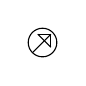
\begin{tikzpicture}
        \draw (0,0) circle (1.2ex);
        \draw (0.7 ex, 0.7 ex) -- (-0.4 ex, 0.7 ex);
        \draw (-0.4 ex, 0.7 ex) -- (0.7 ex, -0.4 ex);
        \draw (0.7 ex, -0.4 ex) -- (0.7 ex, 0.7 ex);
        \draw (0.7 ex, 0.7 ex) -- (-0.848 ex, -0.848 ex);
    \end{tikzpicture}}}
    \ \ 
}

% legendre符号
\makeatletter
\def\legendre@dash#1#2{\hb@xt@#1{%
  \kern-#2\p@
  \cleaders\hbox{\kern.5\p@
    \vrule\@height.2\p@\@depth.2\p@\@width\p@
    \kern.5\p@}\hfil
  \kern-#2\p@
  }}
\def\@legendre#1#2#3#4#5{\mathopen{}\left(
  \sbox\z@{$\genfrac{}{}{0pt}{#1}{#3#4}{#3#5}$}%
  \dimen@=\wd\z@
  \kern-\p@\vcenter{\box0}\kern-\dimen@\vcenter{\legendre@dash\dimen@{#2}}\kern-\p@
  \right)\mathclose{}}
\newcommand\legendre[2]{\mathchoice
  {\@legendre{0}{1}{}{#1}{#2}}
  {\@legendre{1}{.5}{\vphantom{1}}{#1}{#2}}
  {\@legendre{2}{0}{\vphantom{1}}{#1}{#2}}
  {\@legendre{3}{0}{\vphantom{1}}{#1}{#2}}
}
\def\dlegendre{\@legendre{0}{1}{}}
\def\tlegendre{\@legendre{1}{0.5}{\vphantom{1}}}
\makeatother
\addbibresource{Accessories/ref.bib}
\newcommand{\Yang}[1]{\textcolor{red}{#1}}


\title{Notes in Algebraic Geometry}
\author{Tianle Yang}
\date{\today}
\authoremail{\href{mailto:loveandjustice@88.com}{loveandjustice@88.com}}
\authorpage{\href{https://www.tianleyang.com}{www.tianleyang.com}}
\texsource{\href{https://github.com/MonkeyUnderMountain/Note_on_Algebraic_Geometry}{github.com/MonkeyUnderMountain/Note\_on\_Algebraic\_Geometry}}
\version{0.1.0}

\setCJKfamilyfont{lxgwwenkai}{LXGW WenKai} % 定义霞鹜文楷,若未安装,请去掉相关代码编译或使用其他字体
\coversentence{\CJKfamily{lxgwwenkai}「あんたバかァ?」}
\coverimage{Asuka.png} % 封面图片
\coverlinecolor{brown!80!yellow} % 封面横线颜色
\covertitlefont{Allura} % 封面标题字体, 若未安装,可注释掉此行编译或使用其他字体
\covertextcolor{red!80!black} % 封面标题颜色


\begin{document}

    % \pagestyle{empty}
    \maketitle

    \frontmatter

    \tableofcontents

    \mainmatter

    \chapter{Schemes and Varieties}
        \setcounter{section}{-1}
        \section{Locally Ringed Space}

\subsection{Sheaves}

    \begin{definition}\label{def:sheaves}
        Let \(X\) be a topological space.
        A \emph{presheaf} of sets (resp. abelian groups, rings, etc.) on \(X\) is a contravariant functor \(\calF : \Open(X) \to \Set\) (resp. \(\Ab\), \(\Ring\), etc.), 
        where \(\Open(X)\) is the category of open subsets of \(X\) with inclusions as morphisms.

        A presheaf \(\calF\) is a \emph{sheaf} if sections can be glued uniquely.
        More precisely, for every open covering \(\{U_i\}_{i \in I}\) of an open set \(U \subset X\) and every family of sections \(s_i \in \calF(U_i)\) such that \(s_i|_{U_i \cap U_j} = s_j|_{U_i \cap U_j}\) for all \(i,j \in I\),
        there exists a unique section \(s \in \calF(U)\) such that \(s|_{U_i} = s_i\) for all \(i \in I\).
    \end{definition}

    For two open sets \(V \subset U \subset X\), the morphism \(\calF(U) \to \calF(V)\), often denoted by \(\res^U_V\), is called the \emph{restriction map}.

    \begin{example}\label{eg:sheaf_of_smooth_and_analytic_functions}
        Let \(X\) be a real (resp. complex) manifold.
        The assignment \(U \mapsto C^\infty(U, \bbR)\) (resp. \(U \mapsto \{\text{holomorphic functions on }U\}\)) defines a sheaf of rings on \(X\).
    \end{example}

    \begin{example}\label{eg:presheaf_but_not_sheaf}
        Let \(X\) be a non-connected topological space.
        The assignment 
        \[U \mapsto \{\text{constant functions on }U \to \bbR\}\] 
        defines a presheaf \(\calC\) of rings on \(X\) but not a sheaf.

        For a concrete example, let \(X = (0,1)\cup (2,3)\) with the subspace topology from \(\bbR\).
        Consider the open covering \(\{(0,1), (2,3)\}\) of \(X\).
        The sections \(s_1 = 1 \in \calC((0,1))\) and \(s_2 = 2 \in \calC((2,3))\) agree on the intersection (which is empty), 
        but there is no global section \(s \in \calC(X)\) such that \(s|_{(0,1)} = s_1\) and \(s|_{(2,3)} = s_2\).
    \end{example}

    \begin{definition}\label{def:morphism_of_sheaves_and_presheaves}
        Let \(X\) be a topological space and \(\calF, \calG\) be presheaves on \(X\) with values in the same category (e.g., \(\Set\), \(\Ab\), \(\Ring\), etc.).
        A \emph{morphism of presheaves} \(\varphi : \calF \to \calG\) is a natural transformation between the functors \(\calF\) and \(\calG\).
        In other words, for every open set \(U \subset X\), there is a morphism \(\varphi(U) : \calF(U) \to \calG(U)\) such that for every inclusion of open sets \(V \subset U\), the following diagram commutes:
        \[
            \begin{tikzcd}
                \calF(U) \arrow[r, "\varphi(U)"] \arrow[d, "\res^U_V"'] & \calG(U) \arrow[d, "\res^U_V"] \\
                \calF(V) \arrow[r, "\varphi(V)"'] & \calG(V).
            \end{tikzcd}
        \]

        If \(\calF\) and \(\calG\) are sheaves, then \(\varphi\) is called a \emph{morphism of sheaves}.
    \end{definition}

    Fix a topological space \(X\) and a category \(\bfC\).
    The sheaves (resp. presheaves) on \(X\) with values in \(\bfC\) form a category, denoted by \(\Sh(X, \bfC)\) (resp. \(\PSh(X, \bfC)\)), 
    where the objects are sheaves (resp. presheaves) on \(X\) with values in \(\bfC\) and the morphisms are morphisms of sheaves (resp. presheaves).

    \begin{definition}\label{def:stalk_of_sheaves}
        Let \(X\) be a topological space and \(\calF\) a presheaf on \(X\) with values in a category \(\bfC\).
        For a point \(x \in X\), the \emph{stalk} of \(\calF\) at \(x\), denoted by \(\calF_x\), is defined as the colimit
        \[
            \calF_x := \varinjlim_{U \ni x} \calF(U),
        \]
        where the colimit is taken over all open neighborhoods \(U\) of \(x\).
        An element of \(\calF_x\) is called a \emph{germ} of sections of \(\calF\) at \(x\).
    \end{definition}

    More concretely, we have 
    \[ \calF_x = \{(U,s) : U \in \Open(X), U \ni x, s \in \calF(U)\} / \sim, \]
    where \((U,s) \sim (V,t)\) if there exists an open neighborhood \(W \subset U \cap V\) of \(x\) such that \(s|_W = t|_W\).

    \begin{definition}\label{def:sheafification_of_presheaf}
        Let \(X\) be a topological space and \(\calF\) a presheaf on \(X\) with values in \(\Set\) (resp. \(\Ab\), \(\Ring\), etc.).
        A \emph{sheafification} of \(\calF\) is a sheaf \(\calF^\dagger\) on \(X\) together with a morphism of presheaves \(\eta : \calF \to \calF^+\) such that for every sheaf \(\calG\) on \(X\) and every morphism of presheaves \(\varphi : \calF \to \calG\), 
        there exists a unique morphism of sheaves \(\varphi^+ : \calF^+ \to \calG\) such that \(\varphi = \varphi^+ \circ \eta\).
        
        In other words, the following diagram commutes:
        \[
            \begin{tikzcd}
                \calF \arrow[r, "\eta"] \arrow[rd, "\varphi"'] & \calF^\dagger \arrow[d, "\varphi^\dagger"] \\
                & \calG.
            \end{tikzcd}
        \]
        \Yang{To be checked.}
    \end{definition}

    \Yang{The concrete describe of sheafification.}

    % Now we consider \(\Sh(X, \Ab)\).

    \begin{definition}\label{def:injective_and_surjective_of_homomorphism_of_sheaves}
        Let \(X\) be a topological space and \(\varphi : \calF \to \calG\) be a homomorphism of sheaves of abelian groups on \(X\).
        The morphism \(\varphi\) is called \emph{injective} (resp. \emph{surjective}) if for every \(x \in X\), the map \(\varphi_x : \calF_x \to \calG_x\) is injective (resp. surjective).
    \end{definition}

    \begin{proposition}\label{prop:injective_on_section_iff_on_stalk_sheaves}
        Let \(X\) be a topological space and \(\varphi : \calF \to \calG\) be a homomorphism of sheaves of abelian groups on \(X\).
        Then \(\varphi\) is injective if and only if for every open set \(U \subset X\), the map \(\varphi(U) : \calF(U) \to \calG(U)\) is injective.
        \Yang{To be checked.}
    \end{proposition}

    \begin{remark}\label{prop:surjective_on_stalk_cannot_imply_on_sections}
        The surjectivity on stalks cannot imply the surjectivity on sections.
        A counterexample is given by the exponential map \(\exp : \calO_\bbC \to \calO_\bbC^*\) defined by \(\exp(f) = e^{f}\), 
        where \(\calO_\bbC\) is the sheaf of holomorphic functions on \(\bbC\) and \(\calO_\bbC^*\) is the sheaf of non-vanishing holomorphic functions on \(\bbC\).
        The induced map on stalks \(\exp_z : \calO_{\bbC,z} \to \calO_{\bbC,z}^*\) is surjective for every \(z \in \bbC\) by the existence of logarithm locally.
        However, the map on global sections \(\exp(\bbC) : \calO_\bbC(\bbC) \to \calO_\bbC^*(\bbC)\) is not surjective since there is no entire function \(f\) such that \(e^{f(z)} = z\) for all \(z \in \bbC^*\).
        \Yang{To be continued.}
        \Yang{This is wrong, need to be revised.}
    \end{remark}

    \begin{proposition}\label{prop:isomorphism_of_homomorphism_of_sheaves}
        Let \(X\) be a topological space and \(\varphi : \calF \to \calG\) be a homomorphism of sheaves of abelian groups on \(X\).
        Then \(\varphi\) is an isomorphism if and only if it is injective and surjective.
    \end{proposition}

    \Yang{Now we consider sheaves with values in an abelian category.}

    \begin{definition}\label{def:ker_and_cokernel_of_homomorphisms_of_sheaves}
        Let \(X\) be a topological space and \(\varphi : \calF \to \calG\) be a homomorphism of sheaves of abelian groups on \(X\).
        The \emph{kernel} of \(\varphi\), denoted by \(\ker \varphi\), is the sheaf defined by 
        \[
            (\ker \varphi)(U) := \ker(\varphi(U) : \calF(U) \to \calG(U))
        \]
        for every open set \(U \subset X\).

        The \emph{cokernel} of \(\varphi\), denoted by \(\coker \varphi\), is the sheafification of the presheaf defined by 
        \[
            (\coker \varphi)_{\text{pre}}(U) := \coker(\varphi(U) : \calF(U) \to \calG(U))
        \]
        for every open set \(U \subset X\).
        \Yang{To be continued.}
    \end{definition}

    \begin{theorem}\label{thm:sheaves_on_topological_space_is_an_abelian_category}
        Let \(X\) be a topological space and \(\bfC\) be an abelian category (e.g., \(\Ab\)).
        Then the category of sheaves on \(X\) with values in \(\bfC\) is an abelian category.
    \end{theorem}
    \begin{proof}
        \Yang{To be continued.}
    \end{proof}

    \Yang{To be checked and continuous.}


\subsection{Locally ringed space}

       \begin{definition}\label{def:push_forward_of_sheaves}
        Let \(f : X \to Y\) be a continuous map between topological spaces.
        The \emph{push-forward} functor \(f_* : \Sh(X, \bfC) \to \Sh(Y, \bfC)\) is defined by 
        \[
            (f_*\calF)(V) := \calF(f^{-1}(V))
        \]
        for every open set \(V \subset Y\) and sheaf \(\calF \in \Sh(X, \bfC)\).
    \end{definition}
    
    \begin{definition}\label{def:locally_ringed_space}
        A \emph{locally ringed space} is a pair \((X, \calO_X)\) where \(X\) is a topological space and \(\calO_X\) is a sheaf of rings on \(X\) such that for every \(x \in X\), the stalk \(\calO_{X,x}\) is a local ring.
        
        A \emph{morphism of locally ringed spaces} \(f : (X, \calO_X) \to (Y, \calO_Y)\) consists of a continuous map \(f : X \to Y\) and a morphism of sheaves of rings \(f^\sharp : \calO_Y \to f_*\calO_X\) 
        such that for every \(x \in X\), the induced map on stalks \(f_x^\sharp : \calO_{Y,f(x)} \to \calO_{X,x}\) is a local homomorphism, 
        i.e., it maps the maximal ideal of \(\calO_{Y,f(x)}\) to the maximal ideal of \(\calO_{X,x}\).
    \end{definition}

    \begin{example}\label{eg:non_local_homomorphism_of_local_rings}
        Let \(p\) be a prime number.
        Then the inclusion \(\bbZ_{(p)} \to \bbQ\) is a homomorphism of local rings but not a local homomorphism.
        Here \(\bbZ_{(p)}\) is the localization of \(\bbZ\) at the prime ideal \((p)\).
    \end{example}

    \begin{construction}[Glue morphisms]\label{constr:glue_morphisms_of_locally_ringed_spaces}
        Let \(f : (X, \calO_X) \to (Y, \calO_Y)\) be a morphism of locally ringed spaces.
        If \(U \subset X\) and \(V \subset Y\) are open subsets such that \(f(U) \subset V\), then the restriction \(f|_U : (U, \calO_X|_U) \to (V, \calO_Y|_V)\) is a morphism of locally ringed spaces.
        Conversely, if \(\{U_i\}_{i \in I}\) is an open covering of \(X\) and for each \(i \in I\), we have a morphism \(f_i : (U_i, \calO_X|_{U_i}) \to (Y, \calO_Y)\) such that \(f_i|_{U_i \cap U_j} = f_j|_{U_i \cap U_j}\) for all \(i,j \in I\),
        then there exists a unique morphism \(f : (X, \calO_X) \to (Y, \calO_Y)\) such that \(f|_{U_i} = f_i\) for all \(i \in I\).
    \end{construction}

    \begin{construction}[Glue locally ringed space]\label{constr:glue_open_locally_ringed_subspace}
        We construct a locally ringed space by gluing open subspaces.
        Let \((X_i, \calO_{X_i})\) be locally ringed spaces for \(i \in I\) and \((U_{ij}, \calO_{X_i}|_{U_{ij}})\) be open subspaces for \(i,j \in I\).
        Suppose we have isomorphisms \(\varphi_{ij} : (U_{ij}, \calO_{X_i}|_{U_{ij}}) \to (U_{ji}, \calO_{X_j}|_{U_{ji}})\) such that
        \begin{enumerate}
            \item \(\varphi_{ii} = \id_{X_i}\) for all \(i \in I\);
            \item \(\varphi_{ij}(U_{ij} \cap U_{ik}) = U_{ji} \cap U_{jk}\) for all \(i,j \in I\);
            \item \(\varphi_{jk}\circ \varphi_{ij} = \varphi_{ik}\) on \(U_{ij} \cap U_{ik}\) for all \(i,j,k \in I\).
        \end{enumerate}
        Then there exists a locally ringed space \((X, \calO_X)\) and open immersions \(\psi_i : (X_i, \calO_{X_i}) \to (X, \calO_X)\) uniquely up to isomorphism such that 
        \begin{enumerate}
            \item \(\varphi_i(U_{ij}) = \psi_i(X_i)\cap \psi_j(X_j)\) for all \(i,j \in I\);
            \item the following diagram 
                \[ \begin{tikzcd}
                    (U_{ij}, \calO_{X_i}|_{U_{ij}}) \arrow[d, "\varphi_{ij}"'] \arrow[r, hook] & (X_i, \calO_{X_i}) \arrow[r, hook, "\psi_i"] & (X, \calO_X) \arrow[d, "="] \\
                    (U_{ji}, \calO_{X_j}|_{U_{ji}}) \arrow[r, hook] & (X_j, \calO_{X_j}) \arrow[r, hook, "\psi_j"] & (X, \calO_X)
                \end{tikzcd} \]
                commutes for all \(i,j \in I\);
            \item \(X = \bigcup_{i \in I} \psi_i(X_i)\).
        \end{enumerate}
        Such \((X, \calO_X)\) is called \emph{the locally ringed space obtained by gluing the \((X_i, \calO_{X_i})\) along the \(\varphi_{ij}\)}.
        
        First \(\varphi_{ij}\) induces an equivalence relation \(\sim\) on the disjoint union \(\coprod_{i \in I} X_i\).
        By taking the quotient space, we can glue the underlying topological spaces to get a topological space \(X\).
        The structure sheaf \(\calO_X\) is given by 
        \[ \calO_X(V) := \left\{ (s_i)_{i \in I} \in \prod_{i \in I} \calO_{X_i}(\psi_i^{-1}(V)) \;\middle|\; s_i|_{U_{ij}} = \varphi_{ij}^\sharp(s_j|_{U_{ji}}) \text{ for all } i,j \in I \right\}. \]
        Easy to check that \((X, \calO_X)\) is a locally ringed space and satisfies the required properties.
        If there is another locally ringed space \((X', \calO_{X'})\) with \(\psi'_i\) satisfying the same properties, then by gluing \(\psi_i' \circ \psi_i^{-1}\) we get an isomorphism \((X, \calO_X) \to (X', \calO_{X'})\).
    \end{construction}

    \begin{definition}\label{def:closed_and_open_immersion_of_locally_ringed_space}
        A morphism of locally ringed spaces \(f : (X, \calO_X) \to (Y, \calO_Y)\) is called a \emph{closed immersion} (resp. \emph{open immersion}) if 
        \(f\) induces a homeomorphism from \(X\) to a closed (resp. open) subset of \(Y\) and the map \(f^\sharp : \calO_Y \to f_*\calO_X\) is surjective (resp. an isomorphism).
        \Yang{To be checked.}
    \end{definition}



\subsection{Manifolds as locally ringed spaces}


    

\subsection[Vector bundles and O\_X-modules]{Vector bundles and \(\calO_X\)-modules}

    Let \((X,\calO_X)\) be a manifold (real or complex) and \((\calE, \pi, X)\) a vector bundle over \(X\).

    \Yang{It can regard as a sheaf on \(X\).}

    \begin{definition}\label{def:sheaf_of_modules}
        Let \((X,\calO_X)\) be a ringed space.
        A \emph{sheaf of \(\calO_X\)-modules} is a sheaf \(\calF\) of abelian groups on \(X\) such that for every open set \(U\subseteq X\), 
        \(\calF(U)\) is an \(\calO_X(U)\)-module, 
        and for every inclusion of open sets \(V\subseteq U\), the restriction map \(\res_{UV}:\calF(U)\to \calF(V)\) is \(\calO_X(U)\)-linear, 
        where the \(\calO_X(U)\)-module structure on \(\calF(V)\) is induced by the restriction map \(\res_{UV}:\calO_X(U)\to \calO_X(V)\).
        
        A \emph{morphism of \(\calO_X\)-modules} is a morphism of sheaves of abelian groups \(\varphi:\calF\to \calG\) such that 
        for every open set \(U\subseteq X\), the map \(\varphi(U):\calF(U)\to \calG(U)\) is \(\calO_X(U)\)-linear.
        \Yang{To be checked...}
    \end{definition}

    % \Yang{We will try to construct a sequence of subcategories of \(\Mod_{\calO_X}\).}

    % \begin{definition}\label{def:finitely_generated_O_X_modules}
    %     A sheaf of \(\calO_X\)-modules \(\calF\) is said to be \emph{finitely generated} if for every open set \(U \subseteq X\), the \(\calO_X(U)\)-module \(\calF(U)\) is finitely generated.
    %     \Yang{To be continued.}
    % \end{definition}
    
    % \begin{remark}\label{rmk:local_properties_of_sheaves}
    %     There are many versions of ``local'' properties for sheaves of \(\calO_X\)-modules.
    %     \Yang{To be continued.}
    % \end{remark}

    \begin{definition}\label{def:locally_free_O_X_modules}
        A sheaf of \(\calO_X\)-modules \(\calF\) is said to be \emph{locally free of rank \(r\)} if for every point \(x \in X\), there exists an open neighborhood \(U\) of \(x\) such that \(\calF|_U\) is isomorphic to \(\calO_U^r\), 
        where \(\calO_U^r\) is the direct sum of \(r\) copies of \(\calO_U\).
        \Yang{To be continued.}
    \end{definition}

    % \begin{definition}\label{def:quasi_coherent_sheaves}
    %     A sheaf of \(\calO_X\)-modules \(\calF\) is said to be \emph{quasi-coherent} if for every point \(x \in X\), there exists an open neighborhood \(U\) of \(x\) such that \(\calF|_U\) is isomorphic to the cokernel of a morphism of free \(\calO_U\)-modules, i.e., there exists an exact sequence of sheaves of \(\calO_U\)-modules
    %     \[
    %         \calO_U^{(I)} \to \calO_U^{(J)} \to \calF|_U \to 0,
    %     \]
    %     where \(I,J\) are (possibly infinite) index sets.
    %     \Yang{To be checked...}
        
    % \end{definition}

    % \begin{definition}\label{def:coherent_sheaves}
    %     A sheaf of \(\calO_X\)-modules \(\calF\) is said to be \emph{coherent} if it is finitely generated, and for every open set \(U \subseteq X\) and every morphism of sheaves of \(\calO_U\)-modules \(\varphi:\calO_U^n \to \calF|_U\), the kernel of \(\varphi\) is finitely generated.
    %     \Yang{To be checked...}
    % \end{definition}



        \section{The First Properties of Schemes}

If you learn the following content for the first time, it is recommended to skip all the proofs in this section and focus on the examples, remarks and the statements of propositions and theorems.

\subsection{Schemes}

    Let \(R\) be a ring.
    Recall that the \emph{spectrum} of \(R\), denoted by \(\Spec R\), is the set of all prime ideals of \(R\) equipped with the Zariski topology, 
    where the closed sets are of the form \(V(I) = \{\frakp \in \Spec R : I \subset \frakp\}\) for some ideal \(I \subset R\).

    For each \(f \in R\), let \(D(f) = \{\frakp \in \Spec R : f \notin \frakp\}\).
    Such \(D(f)\) is open in \(\Spec R\) and called a \emph{principal open set}.
    
    \begin{proposition}\label{prop:principal_open_sets_form_a_basis}
        Let \(R\) be a ring.
        The collection of principal open sets \(\{D(f) : f \in R\}\) forms a basis for the Zariski topology on \(\Spec R\).
    \end{proposition}
    \begin{proof}
        \Yang{To be continued}
    \end{proof}

    Define a sheaf of rings on \(\Spec R\) by 
    \[ \calO_{\Spec R}(D(f)) = R[1/f]. \]
    Then \((\Spec R, \calO_{\Spec R})\) is a locally ringed space.

    \begin{definition}\label{def:affine_scheme_and_scheme}
        An \emph{affine scheme} is a locally ringed space isomorphic to \((\Spec R, \calO_{\Spec R})\) for some ring \(R\).
        A \emph{scheme} is a locally ringed space \((X, \calO_X)\) which admits an open cover \(\{U_i\}_{i \in I}\) such that \((U_i, \calO_X|_{U_i})\) is an affine scheme for each \(i \in I\).

        A \emph{morphism of schemes} is a morphism of locally ringed spaces.

        These data form a category, denoted by \(\Sch\).
        If we fix a base scheme \(S\), then an \emph{\(S\)-scheme} is a scheme \(X\) together with a morphism \(X \to S\).
        The category of \(S\)-schemes is denoted by \(\Sch/S\) or \(\Sch_S\).
    \end{definition}

    \begin{theorem}\label{thm:equivalence_between_rings_and_affine_schemes}
        The functor \(\Spec : \Ring^{\op} \to \Sch\) is fully faithful and induces an equivalence of categories between the category of rings and the category of affine schemes.
        \Yang{To be continued}
    \end{theorem}

    \begin{definition}\label{def:open_and_closed_immersion}
        A morphism of schemes \(f : X \to Y\) is an \emph{open immersion} (resp. \emph{closed immersion}) if \(f\) induces an isomorphism of \(X\) onto an open (resp. closed) subscheme of \(Y\).
        An \emph{immersion} is a morphism which factors as a closed immersion followed by an open immersion.
        \Yang{To be continued}
    \end{definition}

    \begin{example}\label{eg:projective_scheme_Proj_of_graded_rings_as_schemes}
        Let \(R\) be a graded ring. The \emph{projective scheme} \(\Proj R\) is defined as the scheme associated to the sheaf of rings
        \[
            \mathcal{O}_{\Proj R} = \bigoplus_{d \geq 0} R_d.
        \]
        It can be covered by open affine subschemes of the form \(\Spec R_f\) for homogeneous elements \(f \in R\).
        \Yang{To be checked.}
    \end{example}

    \begin{example}[Glue open subschemes]\label{eg:glue_open_subschemes}
        The construction in \cref{eg:glue_open_locally_ringed_subspace} allows us to glue open subschemes to get a scheme.
        More precisely, let \((X_i, \calO_{X_i})\) be schemes for \(i \in I\) and \((U_{ij}, \calO_{X_i}|_{U_{ij}})\) be open subschemes for \(i,j \in I\).
        Suppose we have isomorphisms \(\varphi_{ij} : (U_{ij}, \calO_{X_i}|_{U_{ij}}) \to (U_{ji}, \calO_{X_j}|_{U_{ji}})\) satisfying the cocycle condition as in \cref{eg:glue_open_locally_ringed_subspace}.
        Then the locally ringed space \((X, \calO_X)\) obtained by gluing the \((X_i, \calO_{X_i})\) along the \(\varphi_{ij}\) is a scheme.
    \end{example}

    \begin{definition}\label{def:scheme_theoretic_image}
        Let \(f : X \to Y\) be a morphism of schemes.
        The \emph{scheme theoretic image} of \(f\) is the smallest closed subscheme \(Z\) of \(Y\) such that \(f\) factors through \(Z\).
        More precisely, if \(Y = \Spec A\) is affine, then the scheme theoretic image of \(f\) is \(\Spec(A/\ker(f^\sharp))\), where \(f^\sharp : A \to \Gamma(X, \calO_X)\) is the induced map on global sections.
        In general, we can cover \(Y\) by affine open subsets and glue the scheme theoretic images on each affine open subset to get the scheme theoretic image of \(f\).
        \Yang{To be checked.}
    \end{definition}

\subsection{Fiber product}

    \begin{definition}\label{def:fiber_product_in_arbitrary_category}
        Let \(\calC\) be a category and \(X, Y, S \in \Obj(\calC)\) with morphisms \(f : X \to S\) and \(g : Y \to S\).
        A \emph{fiber product} of \(X\) and \(Y\) over \(S\) is an object \(Z \in \Obj(\calC)\) together with morphisms \(p : Z \to X\) and \(q : Z \to Y\) such that the following diagram commutes:
        \[
            \begin{tikzcd}
                Z \arrow[r, "q"] \arrow[d, "p"'] & Y \arrow[d, "g"] \\
                X \arrow[r, "f"'] & S
            \end{tikzcd}
        \]
        and satisfies the universal property that for any object \(W \in \Obj(\calC)\) with morphisms \(u : W \to X\) and \(v : W \to Y\) such that \(f \circ u = g \circ v\),
        there exists a unique morphism \(h : W \to Z\) such that \(p \circ h = u\) and \(q \circ h = v\).

        If a fiber product exists, it is unique up to a unique isomorphism.
        We denote the fiber product by \(X \times_S Y\).
        \Yang{To be checked.}
    \end{definition}

    \begin{example}\label{eg:fiber_product_in_sets}
        In the category of sets, the fiber product \(X \times_S Y\) is given by
        \[ X \times_S Y = \{(x,y) \in X \times Y : f(x) = g(y)\}, \]
        with the projections \(p : X \times_S Y \to X\) and \(q : X \times_S Y \to Y\) being the restrictions of the natural projections.
        \Yang{To be checked.}
    \end{example}

    \begin{remark}\label{rmk:fiber_coproduct_and_in_category_of_R_algebras}
        If one reverses the arrows in \cref{def:fiber_product_in_arbitrary_category}, one gets the notion of \emph{fiber coproduct}.
        It is also called the \emph{pushout} or \emph{amalgamated sum} in some literature.
        We denote the fiber coproduct of \(X\) and \(Y\) over \(S\) by \(X \amalg_S Y\).
        Note that in the category of rings, the fiber coproduct \(A \amalg_R B\) of \(R\)-algebras \(A\) and \(B\) over \(R\) is given by the tensor product \(A \otimes_R B\).
        Dually, one can expect that fiber products of affine schemes correspond to tensor products of rings.
    \end{remark}

    \begin{theorem}\label{thm:fiber_product_of_schemes_exists}
        The category of schemes admits fiber products.
        More precisely, given morphisms of schemes \(f : X \to S\) and \(g : Y \to S\), there exists a scheme \(Z\) together with morphisms \(p : Z \to X\) and \(q : Z \to Y\) such that the diagram
        \[
            \begin{tikzcd}
                Z \arrow[r, "q"] \arrow[d, "p"'] & Y \arrow[d, "g"] \\
                X \arrow[r, "f"'] & S
            \end{tikzcd}
        \]
        commutes and satisfies the universal property of the fiber product.
        We denote this scheme by \(X \times_S Y\).
        \Yang{To be continued}
    \end{theorem}

    \begin{definition}\label{def:scheme_theoretic_fiber}
        Let \(f : X \to Y\) be a morphism of schemes and \(y \in Y\) a point.
        The \emph{scheme theoretic fiber} of \(f\) over \(y\) is the fiber product \(X_y = X \times_Y \Spec \kappa(y)\), where \(\kappa(y)\) is the residue field of the local ring \(\calO_{Y,y}\).
        \Yang{To be checked.}
        
    \end{definition}

    \begin{definition}\label{def:scheme_theoretic_intersection}
        Let \(X\) be a scheme and \(Z_1, Z_2 \subset X\) be closed subschemes defined by quasi-coherent sheaves of ideals \(\calI_1, \calI_2 \subset \calO_X\), respectively.
        The \emph{scheme theoretic intersection} of \(Z_1\) and \(Z_2\) is the closed subscheme \(Z_1 \cap Z_2\) defined by the quasi-coherent sheaf of ideals \(\calI_1 + \calI_2\).
        \Yang{To be checked.}
    \end{definition}


\subsection{Noetherian schemes and morphisms of finite type}

    \begin{definition}\label{def:noetherian_scheme}
        A scheme \(X\) is \emph{noetherian} if it admits a finite open cover \(\{U_i\}_{i=1}^n\) such that each \(U_i\) is an affine scheme \(\Spec A_i\) with \(A_i\) a noetherian ring.
        \Yang{To be checked.}
    \end{definition}

    \begin{proposition}\label{prop:noetherian_scheme_is_quasi_compact}
        A noetherian scheme is quasi-compact.
        \Yang{To be checked.}
    \end{proposition}

    \begin{definition}\label{def:scheme_of_finite_type_over_base_scheme}
        Let \(S\) be a scheme.
        A scheme \(X\) is \emph{of finite type} over \(S\) if there exists a finite open cover \(\{U_i\}_{i=1}^n\) of \(S\) such that for each \(i\), \(f^{-1}(U_i)\) can be covered by finitely many affine open subsets \(\{V_{ij}\}_{j=1}^{m_i}\) with \(f(V_{ij}) \subseteq U_i\) and the induced morphism \(f|_{V_{ij}} : V_{ij} \to U_i\) corresponds to a finitely generated algebra over the ring of global sections of \(U_i\).

        \Yang{To be checked.}
    \end{definition}


\subsection{Integral, reduced and irreducible schemes}

    \begin{definition}\label{def:irreducible_topological_space}
        A topological space \(X\) is \emph{irreducible} if it is non-empty and cannot be expressed as the union of two proper closed subsets.
        Equivalently, every non-empty open subset of \(X\) is dense in \(X\).
        \Yang{To be checked.}
    \end{definition}

    \begin{proposition}\label{prop:irreducible_components_and_primary_decomposition}
        Let \(X\) be a topological space satisfying the descending chain condition on closed subsets.
        Then \(X\) can be written as a finite union of irreducible closed subsets, called the \emph{irreducible components} of \(X\).
        Moreover, this decomposition is unique up to permutation of the components.
        \Yang{To be checked.}
    \end{proposition}

    \begin{definition}\label{def:reduced_scheme}
        A scheme \(X\) is \emph{reduced} if its structure sheaf \(\calO_X\) has no nilpotent elements.
        \Yang{To be checked.}
    \end{definition}

    \begin{proposition}\label{prop:reducedness_is_a_local_property}
        A scheme \(X\) is reduced if and only if for every \(x \in X\), the stalk \(\calO_{X,x}\) is a reduced ring.
        \Yang{To be checked.}
    \end{proposition}

    \begin{proposition}\label{prop:universal_property_of_reduced_structure_on_a_scheme}
        Let \(X\) be a scheme.
        There exists a unique closed subscheme \(X_{\red}\) of \(X\) such that \(X_{\red}\) is reduced and has the same underlying topological space as \(X\).
        Moreover, for any morphism of schemes \(f : Y \to X\) with \(Y\) reduced, \(f\) factors uniquely through the inclusion \(X_{\red} \to X\).
        \Yang{To be checked.}
    \end{proposition}

    \begin{definition}\label{def:integral_scheme}
        A scheme \(X\) is \emph{integral} if it is both reduced and irreducible.
        \Yang{To be checked.}
    \end{definition}

    \begin{proposition}\label{prop:integral_scheme_characterization}
        A scheme \(X\) is integral if and only if for every open affine subset \(U = \Spec A \subset X\), the ring \(A\) is an integral domain.
        \Yang{To be checked.}
    \end{proposition}

\subsection{Dimension}

    \begin{definition}\label{def:krull_dimension_of_topological_space}
        The \emph{Krull dimension} of a topological space \(X\), denoted by \(\dim X\), is the supremum of the lengths \(n\) of chains of distinct irreducible closed subsets
        \[ Z_0 \subsetneq Z_1 \subsetneq \cdots \subsetneq Z_n \]
        in \(X\).
        If no such finite supremum exists, we say that \(X\) has infinite dimension.
        \Yang{To be checked.}
    \end{definition}

\subsection{Separated and proper morphisms}

    \begin{definition}\label{def:separated_morphism_and_separated_scheme}
        A morphism of schemes \(f : X \to Y\) is \emph{separated} if the diagonal morphism \(\Delta_f : X \to X \times_Y X\) is a closed immersion.
        A scheme \(X\) is \emph{separated} if the structure morphism \(X \to \Spec \bbZ\) is separated.
        \Yang{To be checked.}
    \end{definition}

    \begin{proposition}\label{prop:affine_scheme_is_separated}
        Any affine scheme is separated.
        More generally, any morphism between affine schemes is separated.
        \Yang{To be checked.}
    \end{proposition}

    \begin{proposition}\label{prop:separatedness_and_rigidity_of_morphisms}
        Let \(f : X \to Y\) be a morphism of schemes.
        Then \(f\) is separated if and only if for any scheme \(T\) and any pair of morphisms \(g_1, g_2 : T \to X\) such that \(f \circ g_1 = f \circ g_2\),
        the equalizer of \(g_1\) and \(g_2\) is a closed subscheme of \(T\).
        \Yang{To be checked.}
    \end{proposition}

    \begin{proposition}\label{prop:separatedness_and_intersection_of_affine_open_subschemes}
        A scheme \(X\) is separated if and only if for any pair of affine open subschemes \(U, V \subset X\), the intersection \(U \cap V\) is also an affine open subscheme.
        \Yang{To be checked.}
    \end{proposition}

    \begin{proposition}\label{prop:composition_and_base_change_of_separated_morphisms}
        The composition of separated morphisms is separated.
        Moreover, separatedness is stable under base change, i.e., if \(f : X \to Y\) is a separated morphism and \(Y' \to Y\) is any morphism, then the base change \(X \times_Y Y' \to Y'\) is also separated.
        \Yang{To be checked.}
        
    \end{proposition}

    \begin{proposition}\label{prop:valuative_criterion_of_separatedness}
        A morphism of schemes \(f : X \to Y\) is separated if and only if for every commutative diagram
        \[
            \begin{tikzcd}
                \Spec K \arrow[r] \arrow[d] & X \arrow[d, "f"] \\
                \Spec R \arrow[r] \arrow[ru, dashed] & Y
            \end{tikzcd}
        \]
        where \(R\) is a valuation ring with field of fractions \(K\), there exists at most one morphism \(\Spec R \to X\) making the entire diagram commute.
        \Yang{To be checked.}
    \end{proposition}

    \begin{definition}\label{def:universally_closed_morphism}
        A morphism of schemes \(f : X \to Y\) is \emph{universally closed} if for any morphism \(Y' \to Y\), the base change \(X \times_Y Y' \to Y'\) is a closed map.
        \Yang{To be checked.}
    \end{definition}

    \begin{definition}\label{def:proper_morphism_and_proper_scheme}
        A morphism of schemes \(f : X \to Y\) is \emph{proper} if it is of finite type, separated, and universally closed (i.e., for any morphism \(Y' \to Y\), the base change \(X \times_Y Y' \to Y'\) is a closed map).
        A scheme \(X\) is \emph{proper} if the structure morphism \(X \to \Spec \bbZ\) is proper.
        \Yang{To be checked.}
    \end{definition}

    \begin{theorem}\label{prop:projective_morphism_is_proper}
        Any projective morphism is proper.
        In particular, any projective scheme is proper.
        \Yang{To be checked.}
    \end{theorem}

    \begin{proposition}\label{prop:composition_and_base_change_of_proper_morphisms}
        The composition of proper morphisms is proper.
        Moreover, properness is stable under base change, i.e., if \(f : X \to Y\) is a proper morphism and \(Y' \to Y\) is any morphism, then the base change \(X \times_Y Y' \to Y'\) is also proper.
        \Yang{To be checked.}
        
    \end{proposition}

    \begin{proposition}\label{prop:valuative_criterion_of_properness}
        A morphism of schemes \(f : X \to Y\) is proper if and only if for every commutative diagram
        \[
            \begin{tikzcd}
                \Spec K \arrow[r] \arrow[d] & X \arrow[d, "f"] \\
                \Spec R \arrow[r] \arrow[ru, dashed] & Y
            \end{tikzcd}
        \]
        where \(R\) is a valuation ring with field of fractions \(K\), there exists a unique morphism \(\Spec R \to X\) making the entire diagram commute.
        \Yang{To be checked.}
        
    \end{proposition}

% \subsection{Projective morphisms}

%     \begin{definition}\label{def:projective_morphisms}
%         Let \(f : X \to Y\) be a morphism of schemes.
%         We say that \(f\) is \emph{projective} if there exists a closed immersion \(i : X \to \bbP^n_Y\) for some \(n \geq 0\) such that the following diagram commutes:
%         \[
%             \begin{tikzcd}
%                 X \arrow[rr, "i"] \arrow[dr, "f"'] & & \bbP^n_Y \arrow[dl, "\pi"] \\
%                 & Y &
%             \end{tikzcd}
%         \]
%         where \(\pi : \bbP^n_Y \to Y\) is the natural projection.
%         \Yang{To be checked.}
%     \end{definition}

%     \begin{theorem}\label{thm:projective_morphism_is_proper}
%         Any projective morphism is proper.
%         In particular, any projective scheme is proper.
%         \Yang{To be checked.}
%     \end{theorem}

%     \begin{definition}\label{def:the_tautological_line_bundle}
%         Let \(Y\) be a scheme. 
%         The \emph{tautological line bundle} \(\mathcal{O}_{\bbP^n_Y}(1)\) is the line bundle on \(\bbP^n_Y\) associated to the divisor corresponding to the hyperplane at infinity.
%     \end{definition}

\subsection{Varieties}
        \section{Category of sheaves of modules}

\subsection{Sheaves of modules, quasi-coherent and coherent sheaves}

    \begin{definition}\label{def:sheaf_of_modules}
        Let $X$ be a ringed space with structure sheaf $\calO_X$. A \textbf{sheaf of (left) $\calO_X$-modules} is a sheaf $\calF$ on $X$ such that for every open set $U\subseteq X$, $\calF(U)$ is an $\calO_X(U)$-module, and for every inclusion of open sets $V\subseteq U$, the restriction map $\rho_{UV}:\calF(U)\to \calF(V)$ is compatible with the restriction map $\rho_{UV}:\calO_X(U)\to \calO_X(V)$ in the sense that for every $s\in \calO_X(U)$ and $m\in \calF(U)$, we have
        \[
            \rho_{UV}(s\cdot m) = \rho_{UV}(s)\cdot \rho_{UV}(m).
        \]
        \Yang{To be continued...}
    \end{definition}

    \begin{example}\label{eg:module_as_sheaf_of_modules_in_affine_case}
        Let $X$ be a scheme. The structure sheaf $\calO_X$ is a sheaf of $\calO_X$-modules. More generally, any quasi-coherent sheaf (to be defined later) is a sheaf of $\calO_X$-modules.
        In particular, if $X=\Spec A$ is an affine scheme, then for any $A$-module $M$, the associated sheaf $\widetilde{M}$ is a sheaf of $\calO_X$-modules.
        \Yang{To be continued...}
    \end{example}

    \begin{definition}\label{def:quasi-coherent_sheaf}
        Let $X$ be a scheme. A sheaf of $\calO_X$-modules $\calF$ is called \textbf{quasi-coherent} if for every point $x\in X$, there exists an open neighborhood $U$ of $x$ such that $\calF|_U$ is isomorphic to the cokernel of a morphism of free $\calO_U$-modules, i.e., there exists an exact sequence of sheaves of $\calO_U$-modules
        \[
            \calO_U^{(I)} \to \calO_U^{(J)} \to \calF|_U \to 0,
        \]
        where $I,J$ are (possibly infinite) index sets.
        \Yang{To be continued...}
    \end{definition}

    \begin{definition}\label{def:coherent_sheaf}
        Let $X$ be a scheme. A sheaf of $\calO_X$-modules $\calF$ is called \textbf{coherent} if it is quasi-coherent and for every point $x\in X$, there exists an open neighborhood $U$ of $x$ such that $\calF|_U$ is isomorphic to the cokernel of a morphism of finite free $\calO_U$-modules, i.e., there exists an exact sequence of sheaves of $\calO_U$-modules
        \[
            \calO_U^m \to \calO_U^n \to \calF|_U \to 0,
        \]
        where $m,n$ are finite integers.
        \Yang{To be continued...}
    \end{definition}

\subsection{As abelian categories}

    \begin{theorem}\label{thm:category_of_sheaves_of_modules_is_abelian}
        Let $X$ be a ringed space. The category of sheaves of $\calO_X$-modules is an abelian category.
        \Yang{To be continued...}
    \end{theorem}

    \begin{theorem}\label{thm:category_of_quasi-coherent_sheaves_is_abelian}
        Let $X$ be a scheme. The category of quasi-coherent sheaves on $X$ is an abelian category.
        \Yang{To be continued...}
    \end{theorem}

    \begin{theorem}\label{thm:category_of_coherent_sheaves_is_abelian}
        Let $X$ be a noetherian scheme. The category of coherent sheaves on $X$ is an abelian category.
        \Yang{To be continued...}
    \end{theorem}

\subsection{Relevant functors}

    \begin{theorem}\label{thm:global_sections_functor}
        Let $X$ be a ringed space. The global sections functor
        \[
            \Gamma(X,-): \text{(Sheaves of $\calO_X$-modules)} \to \text{($\calO_X(X)$-modules)}
        \]
        is left exact.
        \Yang{To be continued...}
    \end{theorem}

    \begin{theorem}\label{thm:direct_image_functor}
        Let $f:X\to Y$ be a morphism of ringed spaces. The direct image functor
        \[
            f_*: \text{(Sheaves of $\calO_X$-modules)} \to \text{(Sheaves of $\calO_Y$-modules)}
        \]
        is left exact.
        \Yang{To be continued...}
    \end{theorem}

    \begin{theorem}\label{thm:inverse_image_functor}
        Let $f:X\to Y$ be a morphism of ringed spaces. The inverse image functor
        \[
            f^*: \text{(Sheaves of $\calO_Y$-modules)} \to \text{(Sheaves of $\calO_X$-modules)}
        \]
        is right exact.
        \Yang{To be continued...}
    \end{theorem}

\subsection{Locally free sheaves and vector bundles}

    \begin{definition}\label{def:locally_free_sheaf}
        Let $X$ be a scheme. A sheaf of $\calO_X$-modules $\calF$ is called \textbf{locally free} if for every point $x\in X$, there exists an open neighborhood $U$ of $x$ such that $\calF|_U$ is isomorphic to a finite free $\calO_U$-module, i.e., there exists an isomorphism of sheaves of $\calO_U$-modules
        \[
            \calF|_U \cong \calO_U^n,
        \]
        where $n$ is a finite integer called the \textbf{rank} of $\calF$ at $x$.
        \Yang{To be continued...}
    \end{definition}

    \begin{example}\label{eg:line_bundle}
        A \textbf{line bundle} on a scheme $X$ is a locally free sheaf of rank 1. The sheaf of differentials $\Omega_{X/k}$ on a smooth variety $X$ over a field $k$ is a locally free sheaf of rank equal to the dimension of $X$.
        \Yang{To be continued...}
    \end{example}

    \begin{theorem}\label{thm:locally_free_sheaf_is_vector_bundle}
        Let $X$ be a scheme. There is an equivalence of categories between the category of locally free sheaves of finite rank on $X$ and the category of vector bundles on $X$.
        \Yang{To be continued...}
    \end{theorem}

\subsection{Cohomological theory}

    \begin{theorem}\label{thm:cohomology_of_sheaves_of_modules}
        Let $X$ be a ringed space and $\calF$ a sheaf of $\calO_X$-modules. Then the cohomology groups $H^i(X,\calF)$ are $\calO_X(X)$-modules for all $i\geq 0$.
        \Yang{To be continued...}
    \end{theorem}

    \begin{theorem}\label{thm:cohomology_of_quasi-coherent_sheaves}
        Let $X$ be a scheme and $\calF$ a quasi-coherent sheaf on $X$. Then the cohomology groups $H^i(X,\calF)$ are $\calO_X(X)$-modules for all $i\geq 0$.
        \Yang{To be continued...}
    \end{theorem}

    \begin{theorem}\label{thm:cohomology_of_coherent_sheaves}
        Let $X$ be a noetherian scheme and $\calF$ a coherent sheaf on $X$. Then the cohomology groups $H^i(X,\calF)$ are $\calO_X(X)$-modules for all $i\geq 0$.
        \Yang{To be continued...}
    \end{theorem}
        \section{Line Bundles and Divisors}

        \section{Morphisms by line bundles and ampleness}



\subsection{Globally generated line bundles}


    \begin{definition}\label{def:gbgs_quasi-coherent_sheaves}
        Let \(X\) be a scheme over a ring \(A\) and \(\calF\) a quasi-coherent sheaf on \(X\).
        We say that \(\calF\) is \emph{globally generated} or \emph{generated by global sections} if the natural map \(\Gamma(X,\calF)\otimes_A \calO_X \to \calF\) is surjective.
    \end{definition}

    \begin{proposition}\label{prop:gbgs_is_stable_under_pullback_tensor_product}
        Let \(X\) be a scheme over a ring \(A\) and \(\calF\), \(\calG\) quasi-coherent sheaves on \(X\).
        Then we have the following:
        \begin{enumerate}
            \item if \(\calF\) is globally generated, then for any morphism \(f:Y\to X\) over \(A\), the pullback \(f^*\calF\) is globally generated on \(Y\);
            \item if both \(\calF\) and \(\calG\) are globally generated, then so is \(\calF \otimes_{\calO_X} \calG\).
        \end{enumerate}
        \Yang{To be revised.}
    \end{proposition}
    
    % \begin{example}\label{eg:multiple_of_globally_generated_line_bundle_is_globally_generated}
    %     Let 
    % \end{example}

    % \begin{example}\label{eg:product_of_pullback_along_natural_projection_is_globally_generated}
        
    % \end{example}

    The story begins with the following theorem, which uses global sections of a globally generated line bundle to construct a morphism to projective space.

    \begin{theorem}\label{thm:morphism_to_projective_space}
        Let \(A\) be a ring and \(X\) an \(A\)-scheme.
        Let \(\calL\) be a line bundle on \(X\) and \(s_0,\ldots,s_n\in\Gamma(X,\calL)\).
        Suppose that \(\{s_i\}\) generate \(\calL\), i.e., \(\bigoplus_i \calO_X\cdot s_i \to \calL\) is surjective.
        Then there is a unique morphism \(f:X\to \bbP^n_A\) such that \(\calL\cong f^*\calO(1)\) and \(s_i=f^*x_i\), where \(x_i\) are the standard coordinates on \(\bbP^n_A\). 
        \Yang{We need a more ``functorial'' expression.}  
    \end{theorem}
    \begin{proof}
        Let \(U_i\coloneqq \{\xi \in X: s_i(\xi) \not\in \frakm_\xi \calL_\xi\}\) be the open subset where \(s_i\) does not vanish.
        Since \(\{s_i\}\) generate \(\calL\), we have \(X=\bigcup_i U_i\).
        Let \(V_i\) be given by \(x_i \neq 0\) in \(\bbP^n_A\).
        On \(U_i\), let \(f_i:U_i\to V_i \subseteq \bbP^n_A\) be the morphism induced by the ring homomorphism
        \[ A\left[\frac{x_0}{x_i},\ldots,\frac{x_n}{x_i}\right] \to \Gamma(U_i,\calO_X), \quad \frac{x_j}{x_i} \mapsto \frac{s_j}{s_i}. \]
        Easy to check that on \(U_i\cap U_j\), \(f_i\) and \(f_j\) agree.
        Thus we can glue them to get a morphism \(f:X\to \bbP^n_A\).
        By construction, we have \(s_i=f^*x_i\) and \(\calL\cong f^*\calO(1)\).
        If there is another morphism \(g:X\to \bbP^n_A\) satisfying the same properties, then on each \(U_i\), \(g\) must agree with \(f_i\) by the same construction.
        Thus \(g=f\).
    \end{proof}

    \begin{example}\label{eg:d-uple_embedding_or_Veronese_embedding}
        Let \(X=\bbP^n_A\) with \(A\) a ring and \(\calL=\calO_{\bbP^n}(d)\) for some \(d>0\).
        Then \(\Gamma(X,\calL)\) is generated by the global sections \(S_{i_0,\ldots,i_n}=T_0^{i_0}T_1^{i_1}\cdots T_n^{i_n}\) for all \((i_0,\ldots,i_n)\) with \(i_0+\cdots+i_n=d\), where \(T_i\) are the standard coordinates on \(\bbP^n\).
        The they induce a morphism \(f:X\to \bbP^N_A\) where \(N=\binom{n+d}{d}-1\).
        If \(A=\kk\) is a field, on \(\kk\)-point level, it is given by
        \[
            [x_0:\cdots:x_n] \mapsto [\ldots:x_0^{i_0}x_1^{i_1}\cdots x_n^{i_n}:\ldots],
        \]
        where the coordinates on the right-hand side are indexed by all \((i_0,\ldots,i_n)\) with \(i_0+\cdots+i_n=d\).
        This is called the \emph{\(d\)-uple embedding} or \emph{Veronese embedding} of \(\bbP^n\) into \(\bbP^N\).
    \end{example}

    \begin{example}\label{eg:Segre_embedding}
        Let \(X=\bbP^m_A \times_A \bbP^n_A\) with \(A\) a ring and \(\calL=\pi_1^*\calO_{\bbP^m}(1) \otimes \pi_2^*\calO_{\bbP^n}(1)\), where \(\pi_1\) and \(\pi_2\) are the projections.
        Let \(T_0,\ldots,T_m\) and \(S_0,\ldots,S_n\) be the standard coordinates on \(\bbP^m\) and \(\bbP^n\) respectively.
        Then \(\Gamma(X,\calL)\) is generated by the global sections \(T_i S_j = \pi_1^*T_i \otimes \pi_2^*S_j\) for \(0\leq i \leq m\) and \(0\leq j \leq n\).
        They induce a morphism \(f:X\to \bbP^{(m+1)(n+1)-1}_A\).
        If \(A=\kk\) is a field, on \(\kk\)-point level, it is given by
        \[ ([x_0:\cdots:x_m],[y_0:\cdots:y_n]) \mapsto [\ldots:x_i y_j:\ldots], \]
        where the coordinates on the right-hand side are indexed by all \((i,j)\) with \(0\leq i \leq m\) and \(0\leq j \leq n\).
        This is called the \emph{Segre embedding} of \(\bbP^m \times \bbP^n\) into \(\bbP^{(m+1)(n+1)-1}\).
    \end{example}

    
    \begin{proposition}\label{prop:different_choices_of_sections_give_different_morphisms_which_differ_by_a_linear_transformation}
        Let \(X\) be a \(\kk\)-scheme for some field \(\kk\) and \(\calL\) is a line bundle on \(X\).
        Suppose that \(\{s_0,\ldots,s_n\}\) and \(\{t_0,\ldots,t_m\}\) span the same subspace \(V\subseteq \Gamma(X,\calL)\) and both generate \(\calL\).
        Let \(f:X\to \bbP^n_\kk\) and \(g:X\to \bbP^m_\kk\) be the morphisms induced by \(\{s_i\}\) and \(\{t_j\}\) respectively.
        Then there exists a linear transformation \(\phi:\bbP^n_\kk \ratmap \bbP^m_\kk\) which is well defined near image of \(f\) and satisfies \(g=\phi \circ f\).
    \end{proposition}
    \begin{proof}
        \Yang{To be continued.}
    \end{proof}


\subsection{Ample line bundles}

    \begin{definition}\label{def:very_ample_line_bundle}
        Let \(X\) be a scheme over a field \(\kk\).
        A line bundle \(\calL\) on a \(X\) is called \emph{very ample} if there exists a closed embedding \(i:X\to \bbP^n_\kk\) such that \(\calL\cong i^*\calO(1)\).
        % \Yang{To be continued.}
    \end{definition}

    The following lemma due to Serre gives a good description of very ample line bundles.

    \begin{lemma}\label{lem:very_ample_and_gbgs}
        Let \(X\) be a scheme over a ring \(A\) and \(\calL\) a very ample line bundle on \(X\).
        Then for any coherent sheaf \(\calF\) on \(X\), there exists an integer \(N\) such that for all \(n \geq N\), \(\calF \otimes \calL^{\otimes n}\) is globally generated.
    \end{lemma}
    \begin{proof}
        \Yang{To be added.}
    \end{proof}

    By \cref{lem:very_ample_and_gbgs}, we have a more intrinsic definition.

    \begin{definition}\label{def:ample_line_bundle}
        A line bundle \(\calL\) on a scheme \(X\) is \emph{ample} if for every coherent sheaf \(\calF\) on \(X\), 
        there exists \(n_0>0\) such that for all \(n\ge n_0\), \(\calF\otimes \calL^{\otimes n}\) is globally generated.
        \Yang{To be continued.}
    \end{definition}
    
    \begin{theorem}\label{thm:ample_very_ample}
        Let \(X\) be a scheme of finite type over a noetherian ring \(A\) and \(\calL\) a line bundle on \(X\).
        Then the following are equivalent:
        \begin{enumerate}
            \item \(\calL\) is ample;
            \item for some \(n>0\), \(\calL^{\otimes n}\) is very ample;
            \item for all \(n \gg 0\), \(\calL^{\otimes n}\) is very ample.
        \end{enumerate}
        \Yang{To be continued.}
    \end{theorem}
    \begin{proof}
        \Yang{To be continued.}
    \end{proof}

    \begin{remark}\label{rmk:define_projective_variety_by_ample_divisors}
        By \cref{thm:ample_very_ample}, a scheme \(X\) which is proper over a field \(\kk\) is projective if and only if it admits an ample line bundle.
        More intrinsically, we will use the definition that a \emph{projective scheme} over a field \(\kk\) is a scheme proper over \(\kk\) which admits an ample line bundle.
        And the ample line bundle is often denoted by \(\calO_X(1)\).
        Once fix the ample line bundle \(\calO_X(1)\), for any coherent sheaf \(\calF\) on \(X\), we denote \(\calF(n) = \calF \otimes \calO_X(n)\) for any integer \(n\).
    \end{remark}

    \begin{proposition}\label{prop:tensor_with_ample_very_ample_and_bpf}
        Let \(X\) be a scheme of finite type over a noetherian ring \(A\) and \(\calL\), \(\calM\) line bundles on \(X\).
        Then we have the following:
        \begin{enumerate}
            \item if \(\calL\) is ample and \(\calM\) is globally generated, then \(\calL \otimes \calM\) is ample;
            \item if \(\calL\) is very ample and \(\calM\) is globally generated, then \(\calL \otimes \calM\) is very ample;
            \item if both \(\calL\) and \(\calM\) are ample, then so is \(\calL \otimes \calM\);
            \item if both \(\calL\) and \(\calM\) are globally generated, then so \(\calL \otimes \calM\);
            \item if \(\calL\) is ample and \(\calM\) is arbitrary, then for some \(n>0\), \(\calL^{\otimes n} \ten \calM\) is ample;
        \end{enumerate}
        \Yang{To be continued.}
    \end{proposition}
    \begin{proof}
        \Yang{To be continued.}
    \end{proof}

    \begin{theorem}[Serre Vanishing]\label{thm:Serre_vanishing}
        Let \(X\) be a projective scheme over a field \(k\) and \(\calL\) a very ample line bundle on \(X\). 
        Then for any coherent sheaf \(\calF\) on \(X\), there exists an integer \(N\) such that for all \(n \geq N\), we have
        \[ H^i(X, \calF \otimes \calL^{\otimes n}) = 0 \]
    \end{theorem}

    \begin{corollary}\label{cor:support_of_ample_divisor_is_connected}
        Let \(X\) be a projective variety over a field \(\kk\) and \(\calL\) an ample line bundle on \(X\).
        Then for any non-zero global section \(s \in \Gamma(X, \calL)\), the support of the effective Cartier divisor \(\divisor(s)\) is connected.
    \end{corollary}

    \begin{definition}\label{def:Hilbert_polynomial_w.r.t_ample_line_bundles}
        Let \((X,\calO_X(1))\) be a projective variety over a field \(\kk\) and \(\calF\) a coherent sheaf on \(X\).
        The \emph{Hilbert polynomial} of \(\calF\) with respect to \(\calO_X(1)\) is the polynomial 
        \[
            P_{\calF}(n) = \chi(X, \calF(n)) = \sum_{i=0}^{\infty} (-1)^i h^i(X, \calF(n)).
        \]
        Let \(Z \subseteq X\) be a closed subscheme with structure sheaf \(\calO_Z\).
        The \emph{Hilbert polynomial} of \(Z\) with respect to \(\calO_X(1)\) is defined as \(P_Z(n) = P_{\calO_Z}(n)\).
        \Yang{To be revised.}
    \end{definition}

    Note that the Euler characteristic \(\chi(X, \calF(n))\) is additive on short exact sequences of coherent sheaves.
    Fix an hypersurface \(H \subseteq X\) defined by a global section of \(\calO_X(1)\).
    Then we have \(\calO_H \cong \calO_X / \calO_X(-1)\).
    Thus by the exact sequence
    \[ 0 \to \calF(n-1) \to \calF(n) \to \calF(n)|_H \to 0, \]
    we have
    \[ P_{\calF}(n) - P_{\calF}(n-1) = P_{\calF|_H}(n). \]
    Inductively, \Yang{...}

    By \cref{thm:Serre_vanishing}, we have 
    \[ P_{\calF}(n) = h^0(X, \calF \otimes \calO_X(n)), \quad \text{for } n \gg 0. \]

    \begin{example}\label{eg:Hilbert_polynomial_of_hypersurfaces}
        Let \(Z \subseteq \bbP^r_\kk\) be a hypersurface of degree \(d\).
        Note that \(h^0(\bbP^r_\kk, \calO_{\bbP^r}(n)) = C^{n+r}_{r}\).
        Then the Hilbert polynomial of \(Z\) with respect to \(\calO_{\bbP^r}(1)\) is
        \[ P_Z(n) = P_{\calO}(n) - P_{\calO(-d)}(n) = \binom{n+r}{r} - \binom{n+r-d}{r} = \frac{d}{(r-1)!} n^{r-1} + \text{lower degree terms}. \]
        \Yang{To be checked.}
    \end{example}



    % \begin{definition}\label{def:semiample_line_bundle}
    %     A line bundle \(\calL\) on a scheme \(X\) is \emph{semiample} if for some \(n>0\), \(\calL^{\otimes n}\) is base-point free.
    %     \Yang{To be continued.}
    % \end{definition}



\subsection{Linear systems}


    In this subsection, when work over a field \(\kk\), we give a more geometric interpretation of previous subsections using the language of linear systems.

    \begin{definition}\label{def:geometric_complete_linear_system}
        Let \(X\) be a normal proper variety over a field \(\kk\), \(D\) a (Cartier) divisor on \(X\) and \(\calL=\calO_X(D)\) the associated line bundle.
        The \emph{complete linear system} associated to \(D\) is the set 
        \[ |D| = \{D'\in \CaDiv(X) : D'\sim D, D' \geq 0\}. \]
    \end{definition}

    There is a natural bijection between the complete linear system \(|D|\) and the projective space \(\bbP(\Gamma(X,\calL))\).
    Here the elements in \(\bbP(\Gamma(X,\calL))\) are one-dimensional subspaces of \(\Gamma(X,\calL)\).
    Consider the vector subspace \(V\subseteq \Gamma(X,\calL)\), we can define the generate linear system \(|V|\) as the image of \(V\setminus \{0\}\) in \(\bbP(\Gamma(X,\calL))\).


    \begin{definition}\label{def:base_locus_and_base_idea}
        Let \(\calL\) be a line bundle on a scheme \(X\).
        \Yang{To be continued.}
    \end{definition}







    % \Yang{The following }



% \subsection{Ample and basepoint free line bundles}



%     \begin{proposition}\label{prop:different_choices_of_sections_give_different_morphisms_which_differ_by_a_linear_transformation}
%         Let \(X\) be a \(\kk\)-scheme for some field \(\kk\) and \(\calL\) is a line bundle on \(X\).
%         Suppose that \(\{s_0,\ldots,s_n\}\) and \(\{t_0,\ldots,t_m\}\) span the same subspace \(V\subseteq \Gamma(X,\calL)\) and both generate \(\calL\).
%         Let \(f:X\to \bbP^n_\kk\) and \(g:X\to \bbP^m_\kk\) be the morphisms induced by \(\{s_i\}\) and \(\{t_j\}\) respectively.
%         Then there exists a linear transformation \(\phi:\bbP^n_\kk \ratmap \bbP^m_\kk\) which is well defined near image of \(f\) and satisfies \(g=\phi \circ f\).
%     \end{proposition}
%     \begin{proof}
%         \Yang{To be continued.}
%     \end{proof}

%     % \begin{example}\label{eg:morphism_induced_by_-K_of_Hirzebruch_surface_F_2}
%     %     Let \(X=\bbF_2\) be the second Hirzebruch surface, i.e., the projective bundle \(\bbP_{\bbP^1}(\calO_{\bbP^1}\oplus \calO_{\bbP^1}(-2))\) over \(\bbP^1\).
%     %     \Yang{To be continued.}
%     % \end{example}

%     % \begin{definition}\label{def:globally_generated_line_bundle}
%     %     A line bundle \(\calL\) on a scheme \(X\) is \emph{globally generated} if \(\Gamma(X,\calL)\) generates \(\calL\), i.e., the natural map \(\Gamma(X,\calL)\otimes \calO_X \to \calL\) is surjective.
%     %     \Yang{To be continued.}
%     % \end{definition}






    

%     % \begin{definition}\label{def:base_locus}
%     %     Let \(\calL\) be a line bundle on a scheme \(X\) and \(V\subseteq \Gamma(X,\calL)\) a subspace.
%     %     The \emph{base locus} of \(V\) is the closed subset
%     %     \[
%     %         \Bs(V) = \{x\in X : s(x)=0, \forall s\in V\}.
%     %     \]
%     %     If \(\Bs(V)=\emptyset\), we say that \(V\) is \emph{base-point free}.
%     %     \Yang{To be continued.}
%     % \end{definition}



%     % \begin{definition}\label{def:linear_system}
%     %     A \emph{linear system} on a scheme \(X\) is a pair \((\calL,V)\) where \(\calL\) is a line bundle on \(X\) and \(V\subseteq \Gamma(X,\calL)\) is a subspace.
%     %     The dimension of the linear system is \(\dim V - 1\).
%     %     A linear system is \emph{base-point free} if \(V\) is base-point free.
%     %     A linear system is \emph{complete} if \(V=\Gamma(X,\calL)\).
%     %     \Yang{To be continued.}
%     % \end{definition}



%     % \begin{proposition}\label{prop:very_ample_iff_separates_points_and_vectors}
%     %     Let \(X\) be a scheme of finite type over a noetherian ring \(A\) and \(\calL\) a line bundle on \(X\).
%     %     Then \(\calL\) is very ample if and only if the following two conditions hold:
%     %     \begin{enumerate}
%     %         \item (separate points) for any two distinct points \(x,y\in X\), there exists \(s\in \Gamma(X,\calL)\) such that \(s(x)=0\) but \(s(y)\neq 0\);
%     %         \item (separate tangent vectors) for any point \(x\in X\) and non-zero tangent vector \(v\in T_xX\), there exists \(s\in \Gamma(X,\calL)\) such that \(s(x)=0\) but \(v(s)\neq 0\).
%     %     \end{enumerate}
%     %     \Yang{To be continued.}
%     % \end{proposition}
    

% \subsection{Linear systems}

    

%     % \begin{definition}\label{def:general_linear_system}
%     %     A \emph{linear system} on a scheme \(X\) is a pair \((\calL,V)\) where \(\calL\) is a line bundle on \(X\) and \(V\subseteq \Gamma(X,\calL)\) is a subspace.
%     %     The dimension of the linear system is \(\dim V - 1\).
%     %     A linear system is \emph{base-point free} if \(V\) is base-point free.
%     %     A linear system is \emph{complete} if \(V=\Gamma(X,\calL)\).
%     %     \Yang{To be continued.}
%     % \end{definition}

%     % \begin{definition}\label{def:base_locus}
%     %     Let \(\calL\) be a line bundle on a scheme \(X\) and \(V\subseteq \Gamma(X,\calL)\) a subspace.
%     %     The \emph{base locus} of \(V\) is the closed subset
%     %     \[
%     %         \Bs(V) = \{x\in X : s(x)=0, \forall s\in V\}.
%     %     \]
%     %     If \(\Bs(V)=\emptyset\), we say that \(V\) is \emph{base-point free}.
%     %     \Yang{To be continued.}
%     % \end{definition}


% \subsection{Asymptotic behavior}

%     \begin{definition}\label{def:section_ring}
%         Let \(X\) be a scheme and \(\calL\) a line bundle on \(X\).
%         The \emph{section ring} of \(\calL\) is the graded ring
%         \[
%             R(X,\calL) = \bigoplus_{n\ge 0} \Gamma(X,\calL^{\otimes n}),
%         \]
%         with multiplication induced by the tensor product of sections.
%         \Yang{To be continued.}
%     \end{definition}


%     \begin{theorem}\label{thm:fibration_associated_to_semiample_line_bundle}
%         Let \(X\) be a scheme over a ring \(A\) and \(\calL\) a semiample line bundle on \(X\).
%         Then there exists a morphism \(f:X\to Y\) over \(A\) such that \(\calL\cong f^*\calO_Y(1)\) for some very ample line bundle \(\calO_Y(1)\) on \(Y\).
%         Moreover, \(Y=\Proj R(X,\calL)\) and \(f\) is induced by the natural map \(R(X,\calL)\to \Gamma(X,\calL^{\otimes n})\).
%         \Yang{To be continued.  }
        
%     \end{theorem}

%     \begin{definition}\label{def:big_line_bundle}
%         A line bundle \(\calL\) on a scheme \(X\) is \emph{big} if the section ring \(R(X,\calL)\) has maximal growth, i.e., there exists \(C>0\) such that
%         \[
%             \dim \Gamma(X,\calL^{\otimes n}) \ge C n^{\dim X}
%         \]
%         for all sufficiently large \(n\).
%         \Yang{To be continued.}
%     \end{definition}

%     \begin{example}\label{eg:base_locus_-K_of_Hirzebruch_surface}
%         Let \(X=\bbF_2\) be the second Hirzebruch surface, i.e., the projective bundle \(\bbP(\calO_{\bbP^1}\oplus \calO_{\bbP^1}(2))\) over \(\bbP^1\).
%         Let \(\pi:X\to \bbP^1\) be the projection and \(E\) the unique section of \(\pi\) with self-intersection \(-2\).
%         \Yang{To be continued.}
%     \end{example}


        \section{Flat, smooth and \'etale morphisms}


\subsection{Flat family and Hilbert polynomial}

    \begin{theorem}\label{thm:flat_iff_has_the_same_Hilbert_polynomials}
        Let \(X\subseteq \bbP^n_T\) be a closed subscheme, where \(T\) is a noetherian scheme. Then the following are equivalent:
        \begin{enumerate}
            \item \(X\to T\) is flat.
            \item The Hilbert polynomial of the fiber \(X_t\subseteq \bbP^n_{k(t)}\) is independent of the choice of \(t\in T\).
        \end{enumerate}
        \Yang{To be checked.}
    \end{theorem}

\subsection{Base change and semicontinuity}

    \begin{theorem}[Base change of flat morphisms]
        Let \(f:X\to Y\) be a flat morphism of schemes. Then for any morphism \(Y'\to Y\), the base change morphism \(f':X\times_Y Y'\to Y'\) is also flat.
    \end{theorem}

    \begin{theorem}[Semicontinuity theorem]
        Let \(f:X\to Y\) be a proper morphism of noetherian schemes, and let \(\calF\) be a coherent sheaf on \(X\) which is flat over \(Y\). Then for each integer \(i\geq 0\), the function
        \[
            h^i:Y\to \bbZ, \quad y\mapsto \dim_{k(y)} H^i(X_y,\calF_y)
        \]
        is upper semicontinuous on \(Y\).
    \end{theorem}
    \Yang{To be checked.}

\subsection{Smooth morphisms}

    \begin{definition}[Smooth morphism]
        A morphism of schemes \(f:X\to Y\) is called \textbf{smooth} at a point \(x\in X\) if there exists an open neighborhood \(U\) of \(x\) such that the restriction \(f|_U:U\to Y\) factors as
        \[
            U \xrightarrow{g} \bbA^n_Y \xrightarrow{p} Y,
        \]
        where \(g\) is \'etale and \(p\) is the projection morphism. The morphism \(f\) is called \textbf{smooth} if it is smooth at every point of \(X\).
    \end{definition}
    \Yang{To be checked.}


\subsection{\'Etale morphisms}

    \begin{definition}[\'Etale morphism]
        A morphism of schemes \(f:X\to Y\) is called \textbf{\'etale} at a point \(x\in X\) if there exists an open neighborhood \(U\) of \(x\) such that the restriction \(f|_U:U\to Y\) factors as
        \[
            U \xrightarrow{g} \bbA^n_Y \xrightarrow{p} Y,
        \]
        where \(g\) is unramified and \(p\) is the projection morphism. The morphism \(f\) is called \textbf{\'etale} if it is \'etale at every point of \(X\).
    \end{definition}
    \Yang{To be checked.}



    \chapter{More Scattered Topics}

    \chapter{Surfaces}
        \section{The first properties of surfaces}

Let \(\kkk\) be an algebraically closed field of arbitrary characteristic.
Unless otherwise specified, all varieties are defined over \(\kkk\).

\subsection{Basic concepts}


\subsection{Riemann-Roch Theorem for surfaces}


\subsection{Hodge Index Theorem}
        \section{Birational geometry on surfaces}

Let \(\kkk\) be an algebraically closed field of arbitrary characteristic.
Unless otherwise specified, all varieties are defined over \(\kkk\).

\subsection{Castelnuovo's Theorem and Run the MMP}

    \begin{theorem}[Castelnuovo's contractibility criterion]\label{thm:castelnuovo_contractibility_criterion}
        Let \(X\) be a smooth projective surface over an algebraically closed field \(\kkk\).
        Let \(C\subseteq X\) be an irreducible curve.
        Then there exists a birational morphism \(f:X\to Y\) contracting \(C\) to a smooth point if and only if \(C\cong \bbP^1\) and \(C^2=-1\).
    \end{theorem}


        \section{Coarse classification of surfaces}

Let \(\kkk\) be an algebraically closed field of arbitrary characteristic.
Unless otherwise specified, all varieties are defined over \(\kkk\).

Let \(X\) be a smooth projective surface over an algebraically closed field \(\kkk\). 
We want to classify \(X\) up to birational equivalence.
Let \(K_X\) be the canonical divisor of \(X\).

% \subsection{Tools}

    \begin{theorem}\label{thm:12K_is_base_point_free_on_surfaces_with_nonnegative_kodaira_dimension}
        Let \(X\) be a smooth projective surface over an algebraically closed field \(\kkk\).
        Suppose that the Kodaira dimension \(\kappa(X)\geq 0\).
        Then the linear system \(|12K_X|\) is base point free.
        \Yang{To be checked.}
    \end{theorem}

\subsection{Classification}

    \begin{theorem}[Enriques-Kodaira classification]\label{thm:enriques_kodaira_classification}
        Let \(X\) be a smooth projective surface over \(\kkk\).
        Then \(X\) is birational to a unique minimal model \(X'\), unless \(X\) is birational to a ruled surface.
        Moreover, the minimal model \(X'\) falls into one of the following classes:
        \begin{enumerate}
            \item \(\kappa(X')=-\infty\): \(X'\cong \bbP^2\) or \(X'\) is a ruled surface;
            \item \(\kappa(X')=0\): \(X'\) is a K3 surface, an abelian surface or their quotients;
            \item \(\kappa(X')=1\): \(X'\) is an elliptic surface;
            \item \(\kappa(X')=2\): \(X'\) is a surface of general type.
        \end{enumerate}
        \Yang{To be checked.}
    \end{theorem}

        \section{Ruled Surface}

In this section, fix an algebraically closed field $\kkk$.

\subsection{Preliminaries}

    Let \(S\) be a variety over \(\kkk\) and \(\calE\) a vector bundle of rank \(r+1\) on \(S\).

    \begin{proposition}\label{prop:isomorphic_projective_bundle_iff_twist_by_line_bundle}
        The \(S\)-varieties \(\bbP_X(\calE) \cong \bbP_X(\calE')\) if and only if \(\calE \cong \calE' \otimes \calL\) for some line bundle \(\calL\) on \(S\).
    \end{proposition}

    \begin{theorem}\label{thm:Eulur_sequence_for_projective_bundle}
        Let \(\pi: X=\bbP_S(\calE) \to S\) be the projective bundle associated to a vector bundle \(\calE\) of rank \(r+1\) on \(S\). 
        Then there is an exact sequence of vector bundles on \(\bbP_S(\calE)\)
        \[
            0 \to \Omega_{\bbP_S(\calE)/S} \to \pi^*(\calE)(-1) \to \calO_{\bbP_S(\calE)} \to 0.
        \]
        In particular, \(K_X \sim \pi^*(K_S + \det \calE) - (r+1)\calO_{\bbP_S(\calE)}(1)\).
        \Yang{To be continued...}
    \end{theorem}

    \begin{theorem}[Tsen's Theorem, {\cite[Tag 03RD]{Stacks}}]\label{thm:Tsen_theorem}
        Let \(C\) be a smooth curve over an algebraically closed field \(\kkk\). 
        Then \(\KK=\kkk(C)\) is a \(C_1\) field, i.e., every degree \(d\) hypersurface in \(\bbP^n_{\KK}\) has a \(\KK\)-rational point provided \(d \leq n\).
        % \Yang{Need a reference.}
    \end{theorem}

    % \begin{theorem}[Cohomology and Base Change, {\cite[Theorem 12.11]{Har77}}]\label{thm:cohomology_and_base_change}
    %     Let \(f:X \to S\) be a projective morphism of noetherian schemes and \(\calF\) a coherent sheaf on \(X\) which is flat over \(S\). 
    %     Then for each \(i \geq 0\) and each point \(s \in S\) there is a natural base change homomorphism
    %     \[
    %         \varphi_s^i: \sfR^i f_*\calF \ten_{\calO_S} \rkk(s) \to H^i(X_s,\calF_s).
    %     \]
    %     Suppose that \(\varphi_s^i\) is surjective. 
    %     Then
    %     \begin{enumerate}
    %         \item there exists an open neighborhood \(U\) of \(s\) such that \(\varphi_{s'}^i\) is an isomorphism for all \(s' \in U\);
    %         \item TFAE:
    %             \begin{enumerate}
    %                 \item \(\varphi_{s}^{i-1}\) is surjective;
    %                 \item \(\sfR^i f_*\calF\) is locally free on an open neighborhood of \(s\).
    %             \end{enumerate}
    %     \end{enumerate}
    % \end{theorem}

    \begin{theorem}[Grauert's Theorem, {\cite[Corollary 12.9]{Har77}}]\label{thm:Grauert_theorem}
        Let \(f:X \to S\) be a projective morphism of noetherian schemes and \(\calF\) a coherent sheaf on \(X\) which is flat over \(S\).
        Suppose that \(S\) is integral and the function \(s \mapsto \dim_{\rkk(s)} H^i(X_s,\calF_s)\) is constant on \(S\) for some \(i \geq 0\). 
        Then \(\sfR^i f_*\calF\) is locally free and the base change homomorphism
        \[
            \varphi_s^i: \sfR^i f_*\calF \ten_{\calO_S} \rkk(s) \to H^i(X_s,\calF_s)
        \]
        is an isomorphism for all \(s \in S\).
    \end{theorem}

    \begin{theorem}[Miracle Flatness, {\cite[Theorem 23.1]{Mat89}}]\label{thm:miracle_flatness}
        Let \(f:X \to Y\) be a morphism of noetherian schemes. 
        Assume that \(Y\) is regular and \(X\) is Cohen-Macaulay. 
        If all fibers of \(f\) have the same dimension \(d = \dim X - \dim Y\), then \(f\) is flat.
    \end{theorem}

    \begin{proposition}[Geometric form of Nakayama's Lemma]\label{prop: geometric form of Nakayama's lemma}
        Let \(X\) be a variety, $x\in X$ a closed point and $\calF$ a coherent sheaf on $X$.
        If $a_1,\cdots,a_k \in \calF(X)$ generate $\calF|_x = \calF \ten \rkk(x)$, then there is an open subset $U \subset X$ such that $a_i|_U$ generate $\calF(U)$. 
    \end{proposition}

    \begin{proposition}\label{prop:relative_projective_morphism}
        Let \(S\) be a noetherian scheme and \(\calE\) a vector bundle of rank \(r+1\) on \(S\). 
        % Then the projection \(\pi:\bbP_X(\calE) \to X\) is a projective morphism.
        Let \(X\) be a \(S\)-scheme via a morphism \(g:X \to S\).
        Then there is a bijection
        \[
            \{S\text{-morphisms } X \to \bbP_S(\calE)\}
            \leftrightarrow
            \left\{
                \begin{array}{l}
                    \text{surjective homomorphisms } g^*\calE \to \calL \\
                    \text{where } \calL \text{ is a line bundle on } X
                \end{array}
            \right\}.
        \]
        \Yang{Need to check.}
    \end{proposition}
    \begin{proof}
        Take an affine cover \(\{U_i\}\) of \(S\) such that \(\calE|_{U_i}\) is trivial.
        On \(U_i\), the surjection \(g^*\calE|_{U_i} \surjmap \calL|_{X_{U_i}}\) gives a morphism \(X_{U_i} \to \bbP_{U_i}(\calE|_{U_i}) \cong \bbP_{S}(\calE)_{U_i}\) by \Yang{ref}.

    \end{proof}

\subsection{Minimal Section and Classification}

    \begin{definition}[Ruled surface]\label{def:ruled_surface}
        A \emph{ruled surface} is a smooth projective surface \(X\) together with a surjective morphism \(\pi:X \to C\) to a smooth curve \(C\) such that all fibers of \(\pi\) are isomorphic to \(\bbP^1\).
    \end{definition}

    Let \(\pi:X \to C\) be a ruled surface over a smooth curve \(C\) of genus \(g\).


    \begin{lemma}\label{lem:existence_of_section_of_ruled_surface}
        There exists a section of \(\pi\).
    \end{lemma}
    \begin{proof}
        \Yang{To be continued...}
    \end{proof}

    \begin{proposition}\label{prop:ruled_surface_as_projective_bundle}
        % Let \(\pi:X \to C\) be a ruled surface over a smooth curve \(C\). 
        Then there exists a vector bundle \(\calE\) of rank \(2\) on \(C\) such that \(X \cong \bbP_C(\calE)\) over \(C\).
    \end{proposition}
    \begin{proof}
        Let \(\sigma:C \to X\) be a section of \(\pi\) and \(D\) be its image.
        Let \(\calL = \calO_X(D)\) and \(\calE = \pi_*\calL\).
        Since \(D\) is a section of \(\pi\), \(\calL|_{X_t} \cong \calO_{\bbP^1}(1)\) for any \(t \in C\), whence \(h^0(X_t,\calL|_{X_t}) = 2\) for any \(t \in C\).
        By Miracle Flatness (\cref{thm:miracle_flatness}), \(f\) is flat.
        By Grauert's Theorem (\cref{thm:Grauert_theorem}), \(\calE\) is a vector bundle of rank \(2\) on \(C\) and we have a natural isomorphism \(\calE \ten \rkk(t) \cong H^0(X_t,\calL|_{X_t})\) for any \(t \in C\).

        This gives a surjective homomorphism 
        \[ \calE \ten_{\calO_C} \rkk(t) \ten_{\rkk(t)} \calO_{X_t} \cong H^0(X_t,\calL|_{X_t}) \ten_{\rkk(t)} \calO_{X_t} \surjmap \calL|_{X_t}. \]
        For every \(x \in X\), we have 
        \[ \calE \ten_{\calO_C} \rkk(\pi(x)) \ten_{\rkk(\pi(x))} \calO_{X_{\pi(x)}} \ten_{\calO_{X_{\pi(x)}}} \rkk(x)  \surjmap \calL|_{X_{\pi(x)}}\ten_{\calO_{X_{\pi(x)}}} \rkk(x). \]
        \Yang{The left side coincides with \(\pi^*\calE\ten_{\calO_X} \rkk(x)\) naturally.}
        Hence by Nakayama's Lemma, the natural homomorphism \(\pi^*\calE \to \calL\) is surjective.

        Denote by \(p: \bbP_C(\calE) \to C\) the projection.
        Take an affine open cover \(\{U_i\}\) of \(C\) such that \(\calE|_{U_i}\) is trivial.
        On \(U_i\), the surjection \(\pi^*\calE|_{X_{U_i}} \surjmap \calL|_{X_{U_i}}\) gives a morphism \(\varphi_i: X_{U_i} \to \bbP_{U_i}(\calE|_{U_i}) \cong \bbP_{C}(\calE)_{U_i}\) by \Yang{ref}.
        Since \(\varphi_i\) and \(\varphi_j\) agree on \(X_{U_i \cap U_j}\), they glue to give a morphism \(\varphi:X \to \bbP_C(\calE)\) over \(C\).
        Since \(\varphi|_{X_t}:X_t \to \bbP_C(\calE)_t\) is an isomorphism for any \(t \in C\), \(\varphi\) is 
        % Since both \(X\) and \(\bbP_C(\calE)\) are smooth, \(\varphi\) is an isomorphism.
    \end{proof}

    \begin{lemma}\label{lem:correspondence_between_sections_and_quotient_line_bundles}
        Fix a vector bundle \(\calE\) of rank \(2\) on \(C\) such that \(X \cong \bbP_C(\calE)\).
        There is a one-to-one correspondence between sections of \(\pi\) and quotient line bundles of \(\calE\) on \(\calC\).
    \end{lemma}
    \begin{proof}
        Suppose we have a quotient \(\calE \to \calL \to 0\) on \(C\) where \(\calL\) is a line bundle on \(C\).
        By \cref{prop:relative_projective_morphism}, we have a morphism \(s:C \to \bbP_C(\calE)\) over \(C\).
        Conversely, let \(\sigma:C \to X\) be a section of \(\pi\) and \(D\) be its image.
    \end{proof}

    \begin{lemma}\label{lem:existence_of_normalized_vector_bundle}
        It is possible to write \(X \cong \bbP_C(\calE)\) such that \(H^0(C,\calE) \neq 0\) but \(H^0(C,\calE \otimes \calL) = 0\) for any line bundle \(\calL\) on \(C\) with \(\deg \calL < 0\).
        Such a vector bundle \(\calE\) is called a \emph{normalized vector bundle}.
    \end{lemma}
    \begin{proof}
        
    \end{proof}

    \begin{definition}\label{def:minimal_section_of_ruled_surface}
        A section \(C_0\) of \(\pi\) is called a \emph{minimal section} if \Yang{to be continued...}
    \end{definition}

    \begin{lemma}\label{thm:restriction_of_e}
        Let \(X=\bbP_C(\calE) \to C\) be a ruled surface over a smooth curve \(C\) of genus \(g\) with invariant \(e\) and normalized \(\calE\). 
        \begin{enumerate}
            \item If \(\calE\) is decomposable, then \(e \geq 0\) and \(\calE \cong \calO_C \oplus \calL\) where \(\calL\) is a line bundle on \(C\) with \(\deg \calL = -e\).
            \item If \(\calE\) is indecomposable, then \(-2g \leq e \leq 2g - 2\).
        \end{enumerate} 
    \end{lemma}

    \begin{theorem}\label{thm:classification_of_ruled_surface_on_P1}
        Let \(\pi:X \to C\) be a ruled surface over \(C = \bbP^1\) with invariant \(e\).
        Then \(X \cong \bbP_{C}(\calO_C \oplus \calO_C(-e))\).
    \end{theorem}

    \begin{example}\label{eg:explicit_description_of_rational_ruled_surface}
        Here we give an explicit description of the ruled surface \(X = \bbP_{\bbP^1}(\calO \oplus \calO(-e))\) for \(e \geq 0\).
        \Yang{To be continued...}
    \end{example}

    \begin{theorem}\label{thm:classification_of_ruled_surface_on_elliptic_curve}
        Let \(\pi:X = \bbP_E(\calE) \to E\) be a ruled surface over an elliptic curve \(E\) with invariant \(e\) and normalized \(\calE\). 
        \begin{enumerate}
            \item If \(\calE\) is indecomposable, then \(e = 0\) or \(-1\), and for each \(e\) there exists a unique such ruled surface up to isomorphism.
            \item If \(\calE\) is decomposable, then \(e \geq 0\) and \(\calE \cong \calO_E \oplus \calL\) where \(\calL\) is a line bundle on \(E\) with \(\deg \calL = -e\).
        \end{enumerate}
    \end{theorem}

    \begin{example}
        \Yang{To be continued...}
    \end{example}


\subsection{The N\'eron-Severi Group of Ruled Surfaces}

    \begin{proposition}\label{prop:Picard_group_of_ruled_surface}
        Let \(\pi:X \to C\) be a ruled surface over a smooth curve \(C\) of genus \(g\). 
        Let \(C_0\) be a minimal section of \(\pi\) and let \(f\) be a fiber of \(\pi\). 
        Then \(\Pic(X) \cong \bbZ C_0 \oplus \pi^*\Pic(C)\).
        \Yang{Check this carefully.}
    \end{proposition}
    \begin{proof}
        \Yang{To be continued...}
    \end{proof}

    \begin{proposition}\label{prop:canonical_divisor_of_ruled_surface}
        Let \(\pi:X \to C\) be a ruled surface over a smooth curve \(C\) of genus \(g\). 
        Let \(C_0\) be a minimal section of \(\pi\) and let \(f\) be a fiber of \(\pi\). 
        Then \(K_X \sim -2C_0 + (K_C-)f\) where \(e = -C_0^2\).
        \Yang{Check this carefully.}
    \end{proposition}
    \begin{proof}
        \Yang{To be continued.}
    \end{proof}

    \paragraph{Rational case.} Let \(\pi:X = \bbP_{\bbP^1}(\calE) \to \bbP^1\) be a ruled surface over \(\bbP^1\) with \(\calE \cong \calO \oplus \calO(-e)\) for some \(e \geq 0\).

    \begin{theorem}\label{thm:positivity_of_divisors_on_rational_ruled_surface}
        Let \(\pi:X \to \bbP^1\) be a ruled surface over \(\bbP^1\) with invariant \(e\).
        Let \(C_0\) be a minimal section of \(\pi\) and let \(F\) be a fiber of \(\pi\). 
        Let \(D \sim aC_0 + bF\) be a divisor on \(X\) with \(a,b \in \bbZ\).
        \begin{enumerate}
            \item \(D\) is ample \(\iff\) \(D\) is very ample \(\iff\) \(a > 0\) and \(b > ae\);
            \item \(D\) is effective \(\iff\) \(a,b \geq 0\).
        \end{enumerate} 
    \end{theorem}
    \begin{proof}
        \Yang{To be continued...}
    \end{proof}


    \paragraph{Elliptic case.} Let \(\pi:X = \bbP_C(\calE) \to E\) be a ruled surface over an elliptic curve \(E\) with \(\calE\) a normalized vector bundle of rank \(2\) and degree \(-e\).

    \begin{theorem}\label{thm:positivity_of_divisors_on_decomposable_ruled_surface_over_elliptic_curve}
        Let \(\pi:X \to E\) be a ruled surface over an elliptic curve \(E\) with invariant \(e\).
        Assume that \(\calE\) is decomposable.
        Let \(C_0\) be a minimal section of \(\pi\) and let \(F\) be a fiber of \(\pi\). 
        Let \(D \equiv aC_0 + bF\) be a divisor on \(X\) with \(a,b \in \bbZ\).
        \begin{enumerate}
            \item \(D\) is ample \(\iff\) \(D\) is very ample \(\iff\) \(a > 0\) and \(b > ae\);
            \item \(D\) is effective \(\iff\) \(a \geq 0\) and \(b \geq ae\).
        \end{enumerate}
    \end{theorem}
    \begin{proof}
        \Yang{To be continued...}
    \end{proof}

    \begin{theorem}\label{thm:positivity_of_divisors_on_indecomposable_ruled_surface_over_elliptic_curve}
        Let \(\pi:X \to E\) be a ruled surface over an elliptic curve \(E\) with invariant \(e\).
        Assume that \(\calE\) is indecomposable.
        Let \(C_0\) be a minimal section of \(\pi\) and let \(F\) be a fiber of \(\pi\). 
        Let \(D \equiv aC_0 + bF\) be a divisor on \(X\) with \(a,b \in \bbZ\).
        \begin{enumerate}
            \item \(D\) is ample \(\iff\) \(D\) is very ample \(\iff\) \(a > 0\) and \(b > \frac{1}{2}ae\);
            \item \(D\) is effective \(\iff\) \(a \geq 0\) and \(b \geq \frac{1}{2}ae\).
        \end{enumerate}
    \end{theorem}
    \begin{proof}
        \Yang{To be continued...}
    \end{proof}


        \section{K3 surface}

Let \(\kkk\) be an algebraically closed field of arbitrary characteristic.
Unless otherwise specified, all varieties are defined over \(\kkk\).


\subsection{The first properties}

    \begin{definition}\label{def:K3_surface}
        A \emph{K3 surface} is a smooth, projective surface \(X\) with trivial canonical bundle \(K_X\cong \calO_X\) and irregularity \(q(X)=h^1(X,\calO_X)=0\).
    \end{definition}

    \begin{example}\label{ex:quartic_in_P3_is_K3}
        A smooth quartic surface \(X\subseteq \bbP^3\) is a K3 surface.
        Indeed, by the adjunction formula, we have
        \[
            K_X = (K_{\bbP^3} + X)|_X = (-4H + 4H)|_X = 0,
        \]
        where \(H\) is a hyperplane in \(\bbP^3\).
        Moreover, by the exact sequence
        \[
            0 \to \calO_{\bbP^3}(-4) \to \calO_{\bbP^3} \to \calO_X \to 0,
        \]
        we have long exact sequence in cohomology
        \[
            \cdots \to H^1(\bbP^3,\calO_{\bbP^3}) \to H^1(X,\calO_X) \to H^2(\bbP^3,\calO_{\bbP^3}(-4)) \to \cdots.
        \]
        Since \(H^1(\bbP^3,\calO_{\bbP^3})=0\) and \(H^2(\bbP^3,\calO_{\bbP^3}(-4))=0\), we get \(H^1(X,\calO_X)=0\).
        % By the Lefschetz hyperplane theorem, we have \(h^1(X,\calO_X)=h^1(\bbP^3,\calO_{\bbP^3})=0\).
        % \Yang{To be checked.}
    \end{example}

\subsection{Hodge Structure and Moduli of K3 surfaces}


\subsection{Neron-Severi group of K3 surfaces}

    
        \section{Elliptic surfaces}


\subsection{The first properties}

    \begin{definition}\label{def:elliptic_surface}
        An \emph{elliptic surface} is a smooth projective surface \(S\) together with a surjective morphism \(\pi:S\to C\) to a smooth projective curve \(C\) such that the generic fiber of \(\pi\) is a smooth curve of genus 1, and \(\pi\) has a section \(s:C\to S\).
        \Yang{To be continued...}
    \end{definition}

\subsection{Classification of singular fibers}


\subsection{Mordell-Weil group and Neron-Severi group}

        \section{Some Singular Surfaces}

In this section, fix an algebraically closed field \(\kkk\).
Everything is over \(\kkk\) unless otherwise specified.

\subsection{Projective cone over smooth projective curve}

    Let \(C \subset \bbP^n\) be a smooth projective curve.
    The \emph{projective cone} over \(C\) is the projective variety \(X \subset \bbP^{n+1}\) defined by the same homogeneous equations as \(C\).
    The variety \(X\) is singular at the vertex of the cone, which corresponds to the point \([0:\cdots:0:1]\in \bbP^{n+1}\).

    \chapter{Moduli of vector bundles on curves}
        \section{Introduction to Moduli Problems}

    Let \(C\) be a smooth projective curve of genus \(g\) over an algebraically closed field \(\kkk\) of characteristic \(0\).

    We are interested in the moduli space of vector bundles on \(C\).

\subsection{Moduli functors}

    Let \(S\) be a noetherian scheme and \(T\) is a scheme of finite type over \(S\).
    Recall the Yoneda lemma: 
    there is a full and faithful functor 
    \[ h : (\Sch_S)^{\op} \to \Fun((\Sch_S)^{\op}, \Set), \quad T \mapsto h_T(S) \coloneqq \Hom_{\Sch_S}(T, S). \]
    
    A functor \(F : (\Sch_S)^{\op} \to \Set\) is \emph{representable} if there exists a scheme \(M\) over \(S\) such that \(F \cong h_M\).
    We say that \(M\) is \emph{the fine moduli space} of \(F\).

    \begin{remark}\label{rmk:fine_moduli_space}
        If \(F\) is representable by \(M\), then there is a universal object \(\calU \in F(M)\) given by \(\id_M \in h_M(M)\) satisfying the following universal property: 
        for any \(T \in \Sch_S\) and any \(\xi \in F(T)\), there exists a unique morphism \(f : T \to M\) such that \(F(f)(\calU) = \xi\).
    \end{remark}

    The most famous example of representable functor is the Quot functor.
    Let \(S\) be a noetherian scheme, \(\pi:X \to S\) a projective morphism, \(\calL\) a relatively ample line bundle on \(X\), \(\calF\) a coherent sheaf on \(X\), and \(P \in \bbQ[t]\) a polynomial.
    We define a functor
    \begin{align*}
        \calQuot_{\calF/X/S}^{P,\calL} : & (\Sch_S)^{\op} \to \Set \\
        & T \mapsto 
        \left\{ 
            \pi^*_T \calF \surjmap \calQ 
        \;\middle|\;
            \calQ \text{ is flat over } T, \forall t \in T, \calQ_t \text{ has Hilbert polynomial } P
        \right\}/ \sim,
    \end{align*}
    where \(\pi^*_T \calF \surjmap \calQ\) and \(\pi^*_T \calF \surjmap \calQ'\) are equivalent if \(\Ker(\pi^*_T \calF \surjmap \calQ) = \Ker(\pi^*_T \calF \surjmap \calQ')\).

    By Grothendieck, \(\calQuot_{\calF/X/S}^{P,\calL}\) is representable by a projective \(S\)-scheme \(\Quot_{\calF/X/S}^{P,\calL}\).
    \Yang{Reference...}

    If we take \(S = \Spec \kkk\), \(X\) a projective variety and \(\calF = \calO_X\).
    Then the Quot functor \(\calQuot_{\calO_X/X/\kkk}^{P,\calL}\) becomes the Hilbert functor \(\calHilb_{X/\kkk}^{P,\calL}\), which is representable by a projective \(\kkk\)-scheme called the \emph{Hilbert scheme} \(\Hilb_X^{P,\calL}\).

\subsection{Moduli functor of vector bundles}

    Consider the functor 
    \begin{align*}
        \tilde{\calM}_{r,d} : & (\Sch_S)^{\op} \to \Set \\
        & T \mapsto \left\{ 
            \calE 
        \;\middle|\;
            \calE \text{ is a vector bundle on } X \times T \text{ of rank } r, \forall t \in T, \deg(\calE_t) = d
         \right\}/ \sim,
    \end{align*}
    where \(\calE \sim \calE'\) if there exists a line bundle \(\calL\) on \(T\) such that \(\calE' \cong \calE \otimes \pi_T^* \calL\), where \(\pi_T : X \times T \to T\) is the projection.

    Unfortunately, \(\tilde{\calM}_{r,d}\) is not representable.
    There are two main reasons:
    \begin{itemize}
        \item unboundedness and 
        \item jumping phenomenon.
    \end{itemize}

    \begin{definition}\label{def:bounded_family}
        A family of vector bundles on a variety \(X\) is \emph{bounded} 
        if there exists a scheme \(S\) of finite type over \(\kkk\) and a vector bundle \(\calE\) on \(X \times S\) 
        such that every vector bundle in the family is isomorphic to \(\calE_s\) for some \(s \in S\).
    \end{definition}

    If \(\tilde{\calM}_{r,d}\) is representable by a scheme \(M\) of finite type over \(\kkk\), then the family of vector bundles parametrized by \(M\) is bounded.
    This is impossible since if so, \(\{h^0(X,\calE) \mid \calE \in \tilde{\calM}_{r,d}(\kkk)\}\) is bounded by semicontinuity theorem, which is not true.
    For example, consider the family \(\calE_n = \calO_X(nP) \oplus \calO_X(-nP) \in \tilde{\calM}_{2,0}(\kkk)\) for \(n \geq 0\), where \(P \in X(\kkk)\) is a fixed point.
    By Riemann-Roch theorem, we have \(h^0(X,\calE_n) = n + 1-g\) for \(n\) sufficiently large.

    \begin{example}\label{eg:Ress_construction}
        Let us see a jumping phenomenon example due to Ress.
        Let \(\calE\) be a vector bundle on \(X\) of rank \(r\) and degree \(d\) with a filtration
        \[F: 0 = \calE_0 \subset \calE_1 \subset \cdots \subset \calE_r = \calE. \]
        On \(X \times \bbA^1\), we can construct a vector bundle \(\calF\) by ``deforming'' \(\calE\) to \(\bigoplus_{i=1}^r \calE_i/\calE_{i-1}\) as follows:
        let \(t\) be the coordinate of \(\bbA^1\), 
        and define \(\calF\) to be the subsheaf of \(\pi_X^* \calE\) generated by \(t^{-i} \cdot \pi_X^* \calE_i\) for \(1 \leq i \leq r\), where \(\pi_X : X \times \bbA^1 \to X\) is the projection.
        Then \(\calF\) is a vector bundle on \(X \times \bbA^1\) of rank \(r\) and degree \(d\).
        We have 
        \[ \calF_t \cong \begin{cases}
            \calE, & t \neq 0, \\
            \bigoplus_{i=1}^r \calE_i/\calE_{i-1}, & t = 0.
        \end{cases} \]
        This is called the \emph{jumping phenomenon}.
        \Yang{To be checked...}

        For a concrete example, let \(X = \bbP^1\), we have an exact sequence
        \[ 0 \to \calO(-2) \to \calO(-1) \oplus \calO(-1) \to \calO \to 0. \]
        Let \(\calE = \calO(-1) \oplus \calO(-1)\) and consider the filtration \(F : 0 \subset \calO(-2) \subset \calE\).
        \Yang{To be continued...}
    \end{example}

    If \(\tilde{\calM}_{r,d}\) is representable by a scheme \(M\), then the family of vector bundles parametrized by \(M\) does not have jumping phenomenon.
    Indeed, if \(\calF\) is an vector bundle on \(X \times \bbA^1\) such that \(\calF_t \cong \calE\) for \(t \neq 0\), 
    then by the universal property of \(M\), there exists a unique morphism \(f : \bbA^1 \to M\) such that \(\calF \cong (\id_X \times f)^* \calU\), 
    where \(\calU\) is the universal vector bundle on \(X \times M\).
    Since \(f\) is constant on the open subset \(\bbA^1 \setminus \{0\}\), it is constant on \(\bbA^1\).
    Thus, \(\calF_0 \cong \calE\).

    To fix the above problems, we need to 
    \begin{itemize}
        \item restrict to a smaller family of vector bundles,
        \item kill jumping phenomenon, and
        \item weaken the notion of representability.
    \end{itemize}

\subsection{Coarse moduli space}

    % \Yang{To be continued...}

    \begin{definition}\label{def:corepresents_functor}
        Let \(F: (\Sch_S)^{\op} \to \Set\) be a functor, \(M\) a scheme over \(S\), and \(\eta : F \to h_M\) a natural transformation.
        We say that \((M, \eta)\) \emph{corepresents} \(F\) 
        if for any scheme \(N\) over \(S\) and any natural transformation \(\eta' : F \to h_N\), 
        there exists a unique morphism \(f : M \to N\) such that the following diagram commutes:
        \[ \begin{tikzcd}
            F \arrow[r, "\eta"] \arrow[dr, "\eta'"'] & h_M \arrow[d, "h_f"] \\
             & h_N.
        \end{tikzcd} \]
    \end{definition}

    \begin{definition}\label{def:coarse_moduli_space}
        A scheme \(M\) over \(S\) is called the \emph{coarse moduli space} of \(F\) if 
        \begin{enumerate}
            \item there exists a natural transformation \(\eta : F \to h_M\) such that \((M, \eta)\) corepresents \(F\);
            \item \(\eta_\kkk : F(\kkk) \to M(\kkk)\) is a bijection.
        \end{enumerate}
    \end{definition}

    \Yang{To be continued...}

\subsection{Semistable vector bundles}

    \begin{proposition}\label{lem:slope_of_exact_sequence}
        Let \(0 \to \calE_1 \to \calE_2 \to \calE_3 \to 0\) be an exact sequence of non-zero vector bundles on \(C\).
        Then \(\mu(\calE_2) \geq \mu(\calE_1)\) (resp. \(\mu(\calE_2) > \mu(\calE_1)\)) if and only if \(\mu(\calE_2) \leq \mu(\calE_3)\) (resp. \(\mu(\calE_2) < \mu(\calE_3)\)).
    \end{proposition}
    \begin{proof}
        We have 
        \[ \mu(\calE_2) = \frac{\deg \calE_2}{\rank \calE_2} = \frac{\deg \calE_1 + \deg \calE_3}{\rank \calE_1 + \rank \calE_3}. \]
        Note that for any \(a,b,c,d \in \bbR_{>0}\), we have 
        \[\frac{a+c}{b+d} \geq \frac{a}{b} \iff bc \geq ad \iff \frac{a+c}{b+d} \leq \frac{c}{d}. \]
        The strict inequality case is similar.
        Then the proposition follows.
    \end{proof}

    \begin{definition}\label{def:stable_and_semistable_vector_bundles_over_curves}
        Let \(C\) be a smooth projective curve over \(\kkk\).
        For a vector bundle \(\calE\) of rank \(r\) and degree \(d\) on \(C\), we define its slope to be \(\mu(\calE) \coloneqq d/r\).
        We say that \(\calE\) is \emph{stable} (resp. \emph{semistable}) if for any proper sub-bundle \(\calF \subset \calE\), we have \(\mu(\calF) < \mu(\calE)\) (resp. \(\mu(\calF) \leq \mu(\calE)\)).
    \end{definition}

    \begin{proposition}\label{prop:homomorphism_between_semistable_and_stable_bundles}
        Let \(\calE\) and \(\calF\) be vector bundles on \(C\).
        Suppose that they are semistable and \(\mu(\calE) > \mu(\calF)\).
        Then any homomorphism \(\varphi : \calE \to \calF\) is zero.

        Suppose that they are stable and \(\mu(\calE) = \mu(\calF)\).
        Then any non-zero homomorphism \(\varphi : \calE \to \calF\) is an isomorphism.
    \end{proposition}
    \begin{proof}
        Let \(\varphi : \calE \to \calF\) be a non-zero homomorphism of vector bundles on \(C\).
        We have an exact sequence
        \[ 0 \to \Ker \varphi \to \calE \to \Image \varphi \to 0. \]
        Since \(\calF\) is vector bundle, hence torsion-free, \(\Image \varphi\) is also torsion-free, thus a vector bundle.

        If \(\calE\) and \(\calF\) are semistable with \(\mu(\calE) > \mu(\calF)\), 
        clearly \(\Ker \varphi \neq 0\), then by \cref{lem:slope_of_exact_sequence}, we have
        \[ \mu(\calE) \leq \mu(\Image \varphi) \leq \mu(\calF). \]
        This is a contradiction, thus \(\varphi = 0\).

        Suppose that \(\calE\) and \(\calF\) are stable with \(\mu(\calE) = \mu(\calF)\).
        If \(\Ker \varphi \neq 0\), then by \cref{lem:slope_of_exact_sequence}, we have
        \[ \mu(\calE) < \mu(\Image \varphi) \leq \mu(\calF). \]
        This is a contradiction, thus \(\varphi\) is injective.
        Since \(\calF\) is stable and \(\Image \varphi \subset \calF\) has the same slope as \(\calF\), we have \(\Image \varphi = \calF\).
    \end{proof}

    \begin{corollary}\label{cor:stable_vector_bundles_are_simple}
        A stable vector bundle is simple as a coherent sheaf, i.e., \(\End(\calE) \cong \kkk\).
    \end{corollary}
    \begin{proof}
        Let \(\varphi \in \End(\calE)\) be a non-zero endomorphism.
        Then there exists \(P \in C(\kkk)\) such that \(\varphi_P : \calE_P \to \calE_P\) is non-zero.
        Let \(a \in \kkk\) be an eigenvalue of \(\varphi_P\) and consider the endomorphism \(\varphi - a \cdot \id_\calE\).
        Then \((\varphi - a \cdot \id_\calE)_P : \calE_P \to \calE_P\) is not an isomorphism, so is \(\varphi - a \cdot \id_\calE\).
        By \cref{prop:homomorphism_between_semistable_and_stable_bundles}, \(\varphi - a \cdot \id_\calE = 0\), thus \(\varphi = a \cdot \id_\calE\).
    \end{proof}

    \begin{lemma}\label{lem:vanishing_and_global_generation_of_semistable_vector_bundles}
        Let \(\calE\) be a semistable vector bundle on \(X\).
        \begin{enumerate}
            \item if \(\mu(\calE) > 2g-2\), then \(H^1(X,\calE) = 0\);
            \item if \(\mu(\calE) > 2g-1\), then \(\calE\) is globally generated.
        \end{enumerate}
    \end{lemma}
    \begin{proof}
        \Yang{To be continued...}
    \end{proof}

    Let \(S_{r,d}\) be set of isomorphism classes of semistable vector bundles on \(X\) of rank \(r\) and degree \(d\).

    \begin{proposition}\label{prop:semistable_vector_bundles_are_bounded}
        The family \(S_{r,d}\) is bounded.
    \end{proposition}
    \begin{proof}
        \Yang{To be continued...}
    \end{proof}


    \begin{definition}[Jordan-H\"older filtration]\label{def:Jordan-Holder_filtration}
        Let \(\calE\) be a semistable vector bundle on \(C\).
        A \emph{Jordan-H\"older filtration} of \(\calE\) is a filtration 
        \[ F : 0 = \calE_0 \subset \calE_1 \subset \cdots \subset \calE_n = \calE \]
        such that \(\calE_i/\calE_{i-1}\) are stable with \(\mu(\calE_i/\calE_{i-1}) = \mu(\calE)\) for all \(1 \leq i \leq n\).
    \end{definition}

    \begin{proposition}\label{prop:existence_and_uniqueness_of_Jordan-Holder_filtration}
        Any semistable vector bundle on \(C\) admits a Jordan-H\"older filtration.
        Moreover, the associated graded object 
        \[ \gr(\calE) \coloneqq \bigoplus_{i=1}^n \calE_i/\calE_{i-1} \]
        is independent of the choice of Jordan-H\"older filtration up to isomorphism.
    \end{proposition}
    \begin{proof}
        \Yang{To be continued...}
    \end{proof}

    \begin{definition}[S-equivalence]\label{def:S-equivalence}
        Two semistable vector bundles \(\calE\) and \(\calF\) of the same rank and degree on \(C\) are called \emph{S-equivalent} 
        if their associated graded objects \(\gr(\calE)\) and \(\gr(\calF)\) (from their Jordan-H\"older filtrations) are isomorphic.
    \end{definition}


    \begin{definition}\label{def:coarse_moduli_functor_of_vector_bundles}
        We define a functor 
        \begin{align*}
            \calM_{r,d}^{ss} : & (\Sch_\kkk)^{\op} \to \Set \\
            & T \mapsto \left\{ 
                \calE 
            \;\middle|\;
                \calE \text{ is a family of semistable vector bundles on } X \text{ of rank } r, \forall t \in T, \deg(\calE_t) = d
            \right\}/ \sim,
        \end{align*}
        where \(\calE \sim \calE'\) if for any \(t \in T\), the vector bundles \(\calE_t\) and \(\calE'_t\) are S-equivalent.
        \Yang{To be continued...}
    \end{definition}

    \chapter{Birational Geometry}
        % \section{Bend and Break}

\subsection{Preliminary}

    \begin{definition}[Frobinius morphism]\label{def:Frobinius_morphism}
        Let \(X\) be a variety over a field \(\kkk\) of characteristic \(p > 0\).
        Denote the structure morphism by \(\pi: X \to \Spec \kkk\).
        The \emph{absolute Frobenius morphism} is the morphism given by \(\calo_X \to \calo_X, f \mapsto f^p\), denoted by \(\Frob_{X/\bbf_p}\).
        The \emph{relative Frobenius morphism} is the morphism \(\Frob_{X/\kkk}\) given by the following commutative diagram:
        \[ \xymatrix{
            X \ar@/^/[rrd]^{\Frob_{X/\bbf_p}}  \ar@/_/[ddr]_\pi \ar[rd]|{\Frob_{X/\kkk}}  &   & \\
                & X\times_{\kkk} \Spec \kkk \ar[r] \ar[d] & X \ar[d]^\pi \\
                & \Spec \kkk \ar[r]^{\Frob_{\kkk/\bbf_p}} &  \Spec \kkk
        }. \] 
        We usually denote \(X \times_{\kkk} \Spec \kkk\) appearing above by \(X^{(p)}\).
    \end{definition}

    \begin{proposition}\label{prop:relative_frobinius_is_finite_of_degree_p^d}
        Let \(X\) be a variety of dimension \(d\) over a field \(\kkk\) of characteristic \(p > 0\).
        Then the relative Frobenius morphism \(\Frob_{X/\kkk}: X \to X^{(p)}\) is a finite morphism of degree \(p^d\) over \(\kkk\).
    \end{proposition}

\subsection{Deformation of curves}

    \begin{theorem}[{ref. \cite[Chapter II, Theorem 1.2]{Kol96}}]\label{thm:dimension_of_deformation_space_of_curves}
        Let \(C\) be a smooth projective curve of genus \(g\) and \(X\) a smooth projective variety of dimension \(n\).
        Let \(f:C \to X\) be a non-constant morphism.
        Then every irreducible component of \(\Mor(C, X)\) containing \(f\) has dimension at least
        \[ -K_Y\cdot f(C) + (1-g)n. \]
    \end{theorem}

    \begin{proposition}\label{prop:deformation_of_curves_to_rational}
        Let \(X\) be a projective variety and \(f:C\to X\) a non-constant morphism from a pointed smooth projective curve \(p_0 \in C\).
        Let \(0 \in T\) be a pointed smooth curve (may not be projective).
        Suppose that we have a non-trivial family of morphisms \(f_t: C \to X\) for \(t \in T\) such that \(f_0 = f\) and \(f_t(p_0) = x_0\) for some point \(x_0 \in X\) and all \(t\).
        Then there exist some rational curves \(\Gamma_1, \ldots, \Gamma_m \subset X\) such that 
        \begin{enumerate}
            \item \(x_0 \in \bigcup_{i=1}^m \Gamma_i\);
            \item there is a morphism \(g: C \to X\) such that \(f(C) \equiv_{alg} g(C) + \sum_{i=1}^m a_i\Gamma_i\) with \(a_i > 0\) for all \(i\).
        \end{enumerate}
    \end{proposition}

    \begin{proposition}\label{prop:deformation_of_rational_curves_to_lower_degree}
        Let \(X\) be a projective variety and \(f:\bbp^1 \to X\) a non-constant morphism with \(f(0) = x_0, f(\infty) = x_\infty\).
        Let \(0 \in T\) be a pointed smooth curve (may not be projective).
        Suppose that we have a non-trivial family of morphisms \(f_t: \bbp^1 \to X\) for \(t \in T\) such that \(f_0 = f\) and \(f_t(0) = x_0, f_t(\infty) = x_\infty\) for all \(t\).
        Then there exists a curve \(C \subset X\) such that \(f(\bbp^1) \equiv_{alg} a C\) with \(a>1\).
    \end{proposition}

\subsection{Find rational curves}

    \begin{theorem}\label{thm:rational_curve_on_smooth_fano}
        Let \(X\) be a smooth Fano variety.
        Then for any \(x \in X(\kkk)\), there is a rational curve \(C\) passing through \(x\) with 
        \[ 0 < - C \cdot K_X \leq \dim X + 1. \]
    \end{theorem}
    \begin{proof}
        \Yang{To be completed.}
    \end{proof}

    \begin{theorem}\label{thm:rational_curve_on_smooth_variety_with_not_nef_K}
        Let \(X\) be a smooth projective variety such that \(K_X \cdot C < 0\) for some irreducible curve \(C \subset X\).
        Let \(H\) be an ample divisor on \(X\).
        Then there exists a rational curve \(\Gamma\) such that
        \[ -(K_X \cdot C) \cdot \frac{H\cdot \Gamma}{H \cdot C} \leq -K_X \cdot \Gamma \leq \dim X + 1. \]
    \end{theorem}
    \begin{proof}
        \Yang{To be completed.}
    \end{proof}

    \begin{theorem}\label{thm:rational_curve_on_exceptional_locus}
        Let \((X,B)\) be a projective klt pair and \(f:X \to Y\) a birational projective morphism.
        Suppose that \(K_{(X,B)}\) is \(f\)-ample.
        Then the exceptional locus of \(f\) is covered by rational curves \(\Gamma\) with 
        \[ 0 < -K_{(X,B)} \cdot \Gamma \leq 2\dim X. \]
    \end{theorem}

    \begin{theorem}\label{thm:general_rational_curve_on_smooth_variety_with_negative_intersection}
        Let \(X\) be a smooth projective variety of dimension \(n\) and \(H, H_1,\cdots,H_{n-1}\) ample divisors on \(X\).
        Suppose that \(K_X\cdot H_1 \cdots H_{n-1} < 0\).
        Then for a general point \(x\in X\), there exists a rational curve \(\Gamma\) passing through \(x\) such that
        \[ 0 < H \cdot \Gamma \leq - 2n \cdot \frac{H\cdot H_1 \cdots H_{n-1}}{K_X \cdot H_1 \cdots H_{n-1}}. \]
    \end{theorem}

    % \begin{proposition}\label{prop:general_rational_curve_on_klt_variety_with_negative_intersection}
    %     Let \(X\) be a normal projective variety of dimension \(n\) and \(H\) an ample divisor on \(X\).
    %     Suppose that \(K_X\cdot H^{n-1} < 0\).
    %     Then for a general point \(x\in X\), there exists a rational curve \(\Gamma\) passing through \(x\) such that
    %     \[ 0 < H \cdot \Gamma \leq - 2n \cdot \frac{H^n}{K_X \cdot H^{n-1}}. \]
    % \end{proposition}
        \section{Technical Preparation}

\subsection{Negativity Lemma}

    \begin{theorem}\label{thm:negativity_lemma}
        Let \(f: Y \to X\) be a proper birational morphism between normal varieties.
        Let \(D\) be a \(\bbQ\)-Cartier \(\bbQ\)-divisor on \(Y\) such that \(-D\) is \(f\)-nef.
        Then \(D\) is effective if and only if \(f_*D\) is.
    \end{theorem}
    \begin{proof}
        \Yang{To be completed.}
    \end{proof}

\subsection{General adjunction formula}

    \begin{theorem}[Adjuction formula]\label{thm:general_adjuction_formula}
        Let \(X\) be a normal variety and \(S\) be a reduced divisor on \(X\).
        % Let \(f: Y \to X\) be a log resolution of \((X,S)\).
        % Write \(K_Y + S' = f^*(K_X + S) + E\), where \(S'\) is the strict transform of \(S\) and \(E\) is exceptional.
        % Then \(f_* \calO_Y(\lceil E \rceil) \cong \calO_X\).
        \Yang{Need to check the statement.}
    \end{theorem}
    \begin{proof}
        \Yang{To be completed.}
    \end{proof}

        \section{Kodaira Vanishing Theorem}

\subsection{Preliminary}

    % \begin{theorem}[GAGA]\label{thm: GAGA for cohomology}
    %     Let $X$ be a smooth projective variety over $\mathbb{C}$ and \(\calF\) a coherent sheaf on \(X\).
    %     Then 
    %     \[
    %         H^i(X, \calF) \cong H^i(X^{an}, \calF^{an}).
    %     \]
    % \end{theorem}

    \begin{theorem}[Serre Duality]\label{thm: Serre duality for line bundles}
        Let \(X\) be a Cohen-Macaulay projective variety of dimension \(n\) over \(\kk\) and \(D\) a divisor on \(X\).
        Then there is an isomorphism
        \[
            H^i(X, D) \cong H^{n-i}(X, K_X - D)^\vee, \quad \forall i = 0, 1, \ldots, n.
        \]
    \end{theorem}

    % \begin{theorem}[Serre Vanishing]\label{thm: Serre vanishing theorem}
    %     Let \(X\) be a proper variety of dimension \(n\) over \(\kk\), \(\calF\) a coherent sheaf and \(\calL\) an ample line bundle on \(X\). 
    %     Then there exists an integer \(m_0 > 0\) such that for all \(m \geq m_0\),
    %     \[
    %         H^i(X, L^m\ten \calF) = 0,\quad \forall i > 0.
    %     \]
    % \end{theorem}

    \begin{theorem}[Log Resolution of Singularities]\label{thm: log resolution of singularities}
        Let X be an irreducible reduced algebraic variety over $\bbC$ (or a suitably small neighborhood of a compact set of an irreducible reduced analytic space) and $I \subset \calO_X$ a coherent sheaf of ideals defining a closed subscheme (or subspace) $Z$. Then there is a smooth variety (or analytic space) $Y$ and a projective morphism $f: Y \to X$ such that
        \begin{enumerate}
            \item $f$ is an isomorphism over $X - (\Sing(X) \cup \Supp Z)$,
            \item $f^*I \subset \calO_Y$ is an invertible sheaf $\calO_Y(-D)$ and 
            \item $\Exc(f) \cup D$ is an snc divisor.
        \end{enumerate}
    \end{theorem}

    \begin{theorem}[Lefschetz Hyperplane Theorem]\label{thm: Lefschetz hyperplane theorem}
        Let \(X\) be a smooth projective variety of dimension \(n\) over \(\bbC\) and \(Y\) a hyperplane section of \(X\).
        Then the restriction map
        \[
            H^k(X,\bbC) \to H^k(Y, \bbC)
        \]
        is an isomorphism for \(k < n - 1\) and an injection for \(k = n - 1\).
    \end{theorem}

    \begin{theorem}[Hodge Decomposition]\label{thm: Hodge decomposition}
        Let \(X\) be a smooth projective variety of dimension \(n\) over \(\bbC\).
        Then for any \(k\), there is a functorial decomposition
        \[
            H^k(X, \bbC) = \bigoplus_{p+q=k} H^{p}(X, \Omega^q_X).
        \]
    \end{theorem}

    Combine Theorem \ref{thm: Lefschetz hyperplane theorem} and Theorem \ref{thm: Hodge decomposition}, we have the following lemma.

    \begin{lemma}\label{lem: Lefschetz hyperplane theorem for cohomology of structure sheaf}
        Let \(X\) be a smooth projective variety of dimension \(n\) over \(\bbC\) and \(Y\) a hyperplane section of \(X\).
        Then the restriction map \(r_k: H^k(X,\bbC) \to H^k(Y, \bbC)\) decomposes as 
        \[
            r_k = \bigoplus_{p+q=k} r_{p,q},\quad r_{p,q}: H^{p}(X, \Omega^q_X) \to H^{p}(Y, \Omega^q_Y).
        \]
        And \(r_{p,q}\) is an isomorphism for \(p + q < n - 1\) and an injection for \(p + q = n - 1\).
        In particular, 
        \[ H^p(X, \calO_X) \to H^p(Y, \calO_Y) \]
        is an isomorphism for \(p < n - 1\) and an injection for \(p = n - 1\).
    \end{lemma}

    \begin{theorem}[Leray spectral sequence]\label{thm: Leray spectral sequence}
        Let \(f: Y \to X\) be a morphism of varieties and \(\calF\) a coherent sheaf on \(Y\).
        Then there is a spectral sequence
        \[
            E_2^{p,q} = H^p(X, R^q f_* \calF) \implies H^{p+q}(Y, \calF).
        \]
    \end{theorem}
        

\subsection{Kodaira Vanishing Theorem}

    \begin{lemma}\label{lem: cyclic covering map in Kodaira Vanishing}
        Let \(X\) be a smooth projective variety over \(\kk\) and \(\calL\) a line bundle on \(X\).
        Suppose there is an integer \(m\) and a smooth divisor \(D \in H^0(X, \calL^m)\).
        Then there exists a finite surjective morphism \(f:Y \to X\) of smooth projective varieties such that \(D':= f^{-1}(D)\) is smooth and satisfies that \(bD' = af^*D\).
    \end{lemma}
    \begin{proof}
        Let \(s \in \calL^m\) be the section defining \(D\).
        It induces a homomorphism \(\calL^{-m} \to \calO_X\).
        Consider the \(\calO_X\)-algebra 
        \[ \calA := \left(\bigoplus_{i = 0}^{\infty} \calL^{-i}\right) \bigg/\left(\calL^{-m} \to \calO_X\right) \cong \bigoplus_{i = 0}^{m-1} \calL^{-i}. \]
        Then \(\calA\) is a finite \(\calO_X\)-algebra.
        Let \(Y \coloneqq \Spec_X \calA\).
        Then \(Y\) is a finite \(\calO_X\)-scheme and the natural morphism \(f: Y \to X\) is finite and surjective.

        For every \(x \in X\), let \(\calL\) locally generated by \(t\) near \(x\).
        Then \(\calO_Y\) locally equal to \(\calO_X[t]/(t^m - s)\).
        Let \(D'\) be the divisor locally given by \(t=0\) on \(Y\).
        Since \(X\) and \(D\) are smooth, then \(Y\) is a smooth variety and \(D'\) is smooth.
        Since \(f\) is finite, it is proper.
        Then \(Y\) is proper and hence \(Y\) is projective.
    \end{proof}
    \begin{remark}\label{rmk: cyclic covering map in Kodaira Vanishing can preverse snc}
        Let \(D_i\) be reduced effective divisors on \(X\) such that \(D + \sum_{i=1}^k D_i\) is snc.
        Set \(D_i' = f^*(D_i)\).
        Then \(D' + \sum_{i=1}^k D_i'\) is snc on \(Y\) by considering the local regular system of parameters.
    \end{remark}

    \begin{lemma}\label{lem: injectivity of cohomology of finite pullback of line bundle}
        Let \(f:Y \to X\) be a finite surjective morphism of projective varieties and \(\calL\) a line bundle on \(X\).
        Suppose that \(X\) is normal.
        Then for any \(i \geq 0\), \(H^i(X,\calL)\) is a direct summand of \(H^i(Y, f^*\calL)\).
    \end{lemma}
    \begin{proof}
        Since \(f\) is finite, we have \(H^i(Y, f^*\calL) \cong H^i(X, f_*\calO_Y \ten \calL)\).
        Since \(X\) are normal, the inclusion \(\calO_X \to f_*\calO_Y\) splits by the trace map \((1/n)\Tr_{Y/X}\).
        Thus we have \(f_*\calO_Y \cong \calO_X \oplus \calF\) and hence 
        \[ H^i(X, f_*\calO_Y \ten \calL) \cong H^i(X, \calL) \oplus H^i(X, \calF \ten \calL). \]
        Then the conclusion follows.
    \end{proof}

    \begin{theorem}[Kodaira Vanishing Theorem]\label{thm: Kodaira Vanishing Theorem}
        Let \(X\) be a smooth projective variety of dimension \(n\) over \(\kk\) of characteristic \(0\) and \(A\) an ample divisor on \(X\). 
        Then
        \[
            H^i(X, \calO_X(-A)) = 0,\quad \forall i < n.
        \]
        Equivalently, we have
        \[
            H^i(X, K_X + A) = 0,\quad \forall i > 0.
        \]
    \end{theorem}
    \begin{proof}
        By Lemma \ref{lem: cyclic covering map in Kodaira Vanishing} and \ref{lem: injectivity of cohomology of finite pullback of line bundle}, after taking a multiple of \(A\), we can assume that \(A\) is effective.
        Then we have an exact sequence
        \[ 0 \to \calO_X(-A) \to \calO_X \to \calO_A \to 0. \]
        Taking the long exact sequence of cohomology, we have
        \[ H^{i-1}(X,\calO_X) \to H^{i-1}(X, \calO_A) \to H^{i}(X, \calO_X(-A)) \to H^{i}(X, \calO_X) \to H^{i}(X, \calO_A). \]
        Then the conclusion follows from Lemma \ref{lem: Lefschetz hyperplane theorem for cohomology of structure sheaf} and Serre duality (Theorem \ref{thm: Serre duality for line bundles}).
    \end{proof}


\subsection{Kawamata-Viehweg Vanishing Theorem}

    We list three versions of Kawamata-Viehweg Vanishing Theorem here.

    \begin{theorem}[Kawamata-Viehweg Vanishing Theorem I]\label{thm: Kawamata-Viehweg Vanishing Theorem for nef and big divisor}
        Let \(X\) be a smooth projective variety of dimension \(n\) over \(\kk\) of characteristic \(0\) and \(D\) a nef and big \(\bbr\)-divisor on \(X\).
        Then 
        \[ H^i(X, K_X + D) = 0,\quad \forall i > 0. \]
    \end{theorem}
    \begin{theorem}[Kawamata-Viehweg Vanishing Theorem II]\label{thm: Kawamata-Viehweg Vanishing Theorem in KM98}
        Let \(X\) be a smooth projective variety of dimension \(n\) over \(\kk\) of characteristic \(0\) and \(D\) a nef and big \(\bbQ\)-divisor on \(X\).
        Suppose that \(\lceil D \rceil - D\) has snc support.
        Then
        \[
            H^i(X, K_X + \lceil D \rceil) = 0,\quad \forall i > 0.
        \]
    \end{theorem}
    \begin{theorem}[Kawamata-Viehweg Vanishing Theorem III]\label{thm: Kawamata-Viehweg Vanishing Theorem for klt pair}
        Let \((X,B)\) be a klt pair over \(\kk\) of characteristic \(0\).
        Let \(D\) be a nef \(\bbQ\)-divisor on \(X\) such that \(D + K_{(X,B)}\) is a Cartier divisor.
        Then
        \[ H^i(X, K_{(X,B)} + D) = 0,\quad \forall i > 0. \]
    \end{theorem}

    If we replace the assumption "nef and big" of \(D\) by "ample" in II and III, we denote them as ``II(ample)'' and ``III(ample)'' respectively.
    Then the proof follows the following line:
    \[ \text{Kodaira Vanishing} \implies \text{II(ample)} \implies \text{III(ample)} \implies \text{I} \implies \text{II} \implies \text{III}. \]
    The proofs leave here and the lemmas used in the proofs are collected in the end of this section.
    
    \begin{proof}[Proof of II (\cref{thm: Kawamata-Viehweg Vanishing Theorem in KM98})]
        Set \(M:= \lceil D \rceil\).
        Let 
        \[ B \coloneqq \sum_{i=1}^k b_i B_i \coloneqq \lceil D \rceil - D = M - A, \quad b_i \in (0,1) \cap \bbQ. \]
        We do not require that \(B_i\) are irreducible but we require that \(B_i\) are smooth.

        We induct on \(k\).
        When \(k = 0\), the conclusion follows from \cref{thm: Kawamata-Viehweg Vanishing Theorem for nef and big divisor}.
        (For the ample case, it follows Kodaira Vanishing Theorem (\cref{thm: Kodaira Vanishing Theorem}.))
        Let \(b_k = a/c\) with lowest terms.
        Then \(a<c\).
        By Lemma \ref{lem: divide a divisor by a finite surjective morphism} and \ref{lem: injectivity of cohomology of finite pullback of line bundle}, we can assume that \((1/c)B_k\) is a Cartier divisor (not necessarily effective).
        Applying Lemma \ref{lem: cyclic covering map in Kodaira Vanishing} on \(B_k\),
        we can find a finite surjective morphism \(f: X' \to X\) such that \(f^*B_k = cB_k', B_i' = f^*B_i\) for \(i < k\) and \(\sum_{i=1}^{k} B_i'\) is an snc divisor on \(X'\).
        Let \(B' = \sum_{i=1}^{k-1}B_i', A' = f^*A\) and \(M' = f^*M\).
        Then \(A'+ B' =  M'-aB_k'\) is Cartier.
        Hence by induction hypothesis, \( H^i(X', -A' - B')\) vanishes for \(i > 0\).
        On the other hand, we have
        \[ \calO_{X'}(-M' + aB_k') \cong \sum_{i=0}^{c-1} f^*\calO_X(-M + (a-i) B_k). \]
        Hence \(H^i(X,\calO_X(-M))\) is a direct summand of \(H^i(X', \calO_{X'}(-M' + aB_k'))\) by Lemma \ref{lem: injectivity of cohomology of finite pullback of line bundle}.
    \end{proof}
    \begin{proof}[Proof of III (\cref{thm: Kawamata-Viehweg Vanishing Theorem for klt pair})]
        Let \(f: \tilde{X} \to X\) be a resolution such that \(\Supp f^*B \cup \Exc f\) is snc.
        We can write
        \[ f^*(K_{(X,B)} + D) + E = K_{(\tilde{X},\tilde{B})} + f^*D, \]
        where \(\tilde{B} \in (0,1)\) has snc support and \(E\) is an effective exceptional divisor.

        By \cref{lem:higher_direct_image_of_exceptional_divisor}, we have 
        \[ H^i(\tilde{X}, K_{(\tilde{X},\tilde{B})} + f^*D) = H^i(X, f_*\calO_Y(f^*(K_{(X,B)}+D)+E)) = H^i(X, K_{(X,B)}+D), \] 
        and the left hand vanishes by \cref{thm: Kawamata-Viehweg Vanishing Theorem in KM98} in either case relative to the assumption of \(D\).
    \end{proof}
    \begin{proof}[Proof of I (\cref{thm: Kawamata-Viehweg Vanishing Theorem for nef and big divisor})]
        By \cref{lem:nef_and_big_approximation_by_ample}, we can choose \(k \gg 0\) such that \((X,1/k B)\) is a klt pair with \(D \sim_\bbQ A + \frac{1}{k}B\) for some ample divisor \(A\).
        Then the theorem comes down to \cref{thm: Kawamata-Viehweg Vanishing Theorem for klt pair}.
    \end{proof}

    \begin{lemma}\label{lem:higher_direct_image_of_exceptional_divisor}
        Let \(f:Y \to X\) be a birational morphism of projective varieties with \(Y\) smooth and \(X\) has only rational singularities.
        Let \(E\) be an effective exceptional divisor on \(Y\) and \(D\) a divisor on \(X\).
        Then we have
        \[ f_*(\calO_Y(f^*D + E)) \cong \calO_X(D), \quad R^if_*(\calO_Y(f^*D + E)) = 0,\quad \forall i > 0. \]
    \end{lemma}
    \begin{proof}
        \Yang{I am unable to proof this lemma.}
    \end{proof}

    \begin{lemma}\label{lem: divide a divisor by a finite surjective morphism}
        Let \(X\) be a projective variety, \(\calL\) a line bundle on \(X\) and \(m \in \bbZ_{\geq 0}\).
        Then there exists a finite surjective morphism \(f: Y \to X\) and a line bundle \(\calL'\) on \(Y\) such that \(f^*\calL \sim \calL'^{m}\).
        If \(X\) is smooth, then we can take \(Y\) to be smooth.
        Moreover, if \(D = \sum D_i\) is an snc divisor on \(X\), then we can take \(f\) such that \(f^*D\) is an snc divisor on \(Y\).
    \end{lemma}
    \begin{proof}
        We can assume that \(\calL\) is very ample by writing it as a difference of two very ample line bundles.
        Consider the fiber product \(Y:= \bbp^N \times_{\bbp^N} X\) as the following diagram
        \[ \xymatrix{
            Y \ar[r]^{\psi} \ar[d]_{f} & \mathbb{P}^N \ar[d]^{g} \\
            X \ar[r]^{\varphi_\calL} & \mathbb{P}^N
        }, \]
        where \(g: [x_0: \ldots: x_N] \mapsto [x_0^m: \ldots: x_N^m]\).
        The morphism \(f\) is finite and surjective since so is \(g\).
        Let \(\calL'\coloneqq \psi^*\calL\).

        For smoothness, we can compose \(g\) with a general automorphism of \(\bbp^N\).
        Then the conclusion follows from \cite[Chapter III, Theorem 10.8]{Har77}.
    \end{proof}

    \begin{lemma}[{ref. \cite[Theorem 5.10, 5.22]{KM98}}]\label{lem: klt pair has rational singularities and is Cohen-Macaulay}
        Let \((X,B)\) be a klt pair over \(\kk\) of characteristic \(0\).
        Then \(X\) has rational singularities and is Cohen-Macaulay.
    \end{lemma}

    \begin{lemma}\label{lem:nef_and_big_approximation_by_ample}
        Let \(X\) be a projective variety of dimension \(n\) and \(D\) a nef and big divisor on \(X\).
        Then there exists an effective divisor \(B\) such that for every \(k\), there is an ample divisor \(A_k\) such that 
        \[ D \sim_\bbQ A_k + \frac{1}{k}B. \]
    \end{lemma}
    \begin{proof}
        By \Yang{definition} of big divisor, there exists an ample divisor \(A_1\) and effective divisor \(B\) such that
        \[ D \sim_\bbQ A_1 + B. \]
        Then we have 
        \[ D \sim_\bbQ \frac{A + (k-1)D}{k} + \frac{1}{k}B. \]
        Since \(A\) is ample and \(D\) is nef, we can take \(A_k = (A + (k-1)D)/k\) which is ample.
        % \Yang{To be completed.}
    \end{proof}
 
    
    % \begin{lemma}\label{lem: vanishing for ample plus snc divisor}
    %     Let \(X\) be a smooth projective variety of dimension \(n\) over \(\kk\) of characteristic \(0\), \(A\) an ample divisor and \(E\) an snc divisor on \(X\).
    %     % Suppose that \(E\) is an effective divisor on \(X\) with snc support.
    %     Then
    %     \[
    %         H^i(X, K_X + A + E) = 0,\quad \forall i > 0.
    %     \]
    % \end{lemma}
    % \begin{proof}
    %     Let \(E = \sum_{i=1}^k E_i\).
    %     We induct on \(k\).
    %     Consider the exact sequence
    %     \[ 0 \to \calO_X(-A-\sum_{i=1}^{k} E_i) \to \calO_X(-A-\sum_{i=1}^{k-1} E_i) \to \calO_{E_k}(-A-\sum_{i=1}^{k-1} E_i) \to 0. \]
    %     \Yang{To be completed.}
    % \end{proof}
        \section{Cone Theorem}


\subsection{Preliminary}

    \begin{theorem}[{Iitaka fibration, semiample case, ref. \cite[Theorem 2.1.27]{Laz04a}}]\label{thm: Iitaka fibration in semiample case}
        Let \(X\) be a projective variety and \(\call\) an semiample line bundle on \(X\).
        Then there exists a fibration \(\varphi: X \to Y\) of projective varieties 
        such that for any \(m\gg 0\) with \(\call^m\) base point free, we have that the morphism \(\varphi_{\call^m}\) induced by \(\call^m\) is isomorphic to \(\varphi\).
        Such a fibration is called the \emph{Iitaka fibration} associated to \(\call\).
    \end{theorem}

    \begin{theorem}[{Rigidity Lemma, ref. \cite[Lemma 1.15]{Deb01}}]\label{thm: Rigidity Lemma}
        Let \(\pi_i: X \to Y_i\) be proper morphisms of varieties over a field \(\kk\) for \(i=1,2\).
        Suppose that \(\pi_1\) is a fibration and \(\pi_2\) contracts \(\pi_1^{-1}(y_0)\).
        Then there exists a rational map \(\varphi: Y_1 \ratmap Y_2\) such that \(\pi_2 \circ \varphi = \pi_1\) and \(\varphi\) is well-defined near \(Y_1 \setminus \{y_0\}\). 
    \end{theorem}

    \begin{theorem}\label{thm:convex_separation_theorem}
        Let \(A,B \subset \bbr^n\) be disjoint convex sets.
        Then there exists a linear functional \(f: \bbr^n \to \bbr\) such that \(f|_A \leq c\) and \(f|_B \geq c\) for some \(c \in \bbr\).
    \end{theorem}

    % \begin{theorem}[{Upper semicontinuity of cohomology, ref. \cite[Chapter III, Theorem 12.8]{Har77}}]\label{thm: upper semicontinuity of cohomology}
    %     Let \(f:X \to Y\) be a projective morphism of noetherian schemes and \(\calf\) a coherent sheaf on \(X\) flat over \(Y\).
    %     Then the function \(y \mapsto h^i(y,\calf)\) is upper semicontinuous on \(Y\) for every \(i\).   
    % \end{theorem}

    % \begin{theorem}[{Grauert's Theorem, ref. \cite[Chapter III, Corollary 12.9]{Har77}}]\label{thm: Grauert's Theorem}
    %     Let \(f:X \to Y\) be a projective morphism of noetherian schemes and \(\calf\) a coherent sheaf on \(X\) flat over \(Y\).
    %     Suppose that \(Y\) is integral and \(h^i(y,\calf)\) is constant on \(Y\) for some \(i\).
    %     Then \(R^if_*\calf\) is locally free sheaf on \(Y\) and the natural map \(R^if_*\calf \ten \rkk(y) \to H^i(X_y,\calf_y)\) is an isomorphism for every \(y \in Y\).
    % \end{theorem}

\subsection{Non-vanishing Theorem}

    \begin{theorem}[Non-vanishing Theorem]\label{thm: non-vanishing theorem}
        Let \((X,B)\) be a projective klt pair and \(D\) a Cartier divisor on \(X\).
        Suppose that \(D\) is nef and \(aD-K_{(X,B)}\) is nef and big for some \(a > 0\).
        Then for \(m \gg 0\), we have 
        \[ H^0(X,mD) \neq 0. \]
    \end{theorem}

\subsection{Base Point Free Theorem}

    \begin{theorem}[Base Point Free Theorem]\label{thm: base point free theorem}
        Let \((X,B)\) be a projective klt pair and \(D\) a Cartier divisor on \(X\).
        Suppose that \(D\) is nef and \(aD-K_{(X,B)}\) is nef and big for some \(a > 0\).
        Then for \(m \gg 0\), \(mD\) is base point free.
    \end{theorem}

    \begin{remark}\label{rmk:statement_in_BPF_theorem_stronger_than_semiample}
        In general, we say that a Cartier divisor \(D\) is \emph{semiample} if there exists a positive integer \(m\) such that \(mD\) is base point free.
        The statement in Base Point Free Theorem (\cref{thm: base point free theorem}) is strictly stronger than the semiample condition.
        For example, let \(\call\) be a torsion line bundle, then \(\call\) is semiample but there exists no positive integer \(M\) such that \(m\call\) is base point free for all \(m>M\).
    \end{remark}

\subsection{Rationality Theorem}

    \begin{theorem}[Rationality Theorem]\label{thm: rationality theorem}
        Let \((X,B)\) be a projective klt pair, \(a = a(X) \in \bbz\) with \(aK_{(X,B)}\) Cartier and \(H\) an ample divisor on \(X\).
        Let 
        \[ t \coloneqq \inf \{s \geq 0: K_{(X,B)} + sH \text{ is nef}\} \]
        be the nef threshold of \((X,B)\) with respect to \(H\).
        Then \(t = u/v \in \bbq\) and 
        \[ 0 \leq u \leq a(X)\cdot (\dim X + 1). \]
    \end{theorem}


\subsection{Cone Theorem and Contraction Theorem}

    \begin{theorem}[Cone Theorem]\label{thm: cone theorem}
        Let \((X,B)\) be a projective klt pair.
        Then there exist countably many rational curves \(C_i \subset X\) with 
        \[ 0 < -K_{(X,B)} \cdot C_i \leq 2 \dim X \]
        such that 
        \begin{enumerate}
            \item we have a decomposition of cones
            \[ \Psef_1(X) = \Psef_1(X)_{K_{(X,B)} \geq 0} + \sum \bbr_{\geq 0}[C_i]; \]
            \item and for any \(\varepsilon > 0\) and an ample divisor \(H\) on \(X\), we have 
            \[ \Psef_1(X) = \Psef_1(X)_{K_{(X,B)}+\varepsilon H \geq 0} + \sum_{\text{finite}} \bbr_{\geq 0}[C_i]. \]
        \end{enumerate}
    \end{theorem}
    \begin{proof}
        Let \(F_D \coloneqq \Psef_1(X) \cap D^\perp\) for a nef divisor \(D\) on \(X\).
        If \(\dim F_D = 1\), we also write \(R_D \coloneqq F_D\).
        Let \(H_1,\cdots,H_{\rho-1}\) be ample divisors on \(X\) such that they together with \(K_{(X,B)}\) form a basis of \(N^1(X)_\bbr\).
        Let \(S^{\rho-1} \coloneqq S(N_1(X)_\bbr)\) be the unit sphere in \(N_1(X)_\bbr\).
        
        \begin{step}\label{step_in_thm:cone_theorem:nagetive_extremal_rays_form_a_lattice}
            Let \(\Phi: N_1(X)_{K_{(X,B)}<0} \to \bbr^{\rho-1}\) be the map defined by 
            \[ [C] \mapsto \left( \frac{H_1 \cdot C}{K_{(X,B)}\cdot C},\ldots, \frac{H_{\rho-1} \cdot C}{K_{(X,B)}\cdot C}\right). \]
            We show that the image of \(R_D\) under \(\Phi\) lying a \(\bbz\)-lattice in \(\bbr^{\rho-1}\).
        \end{step}
        \Yang{To be completed.}

        \begin{step}\label{step_in_thm:cone_theorem:negative_extremal_rays_are_rational}
            We show that every \(K_{(X,B)}\)-negative extremal ray of \(\Psef_1(X)\) is of the form \(R_D\) for some nef divisor \(D\) on \(X\).
        \end{step}
        \Yang{To be completed.}

        \begin{step}\label{step_in_thm:cone_theorem:nagetive_extremal_rays_have_class_of_rational_curves}
            We show that any \(K_{(X,B)}\)-negative extremal ray \(R_D\) contains the class of a rational curve \(C\) with \(0 < -K_{(X,B)} \cdot C \leq 2 \dim X\).
        \end{step}

        \Yang{To be completed.}

        \begin{step}\label{step_in_thm:cone_theorem:finish_the_proof}
            Proof of the theorem.
        \end{step}
        Given an ample divisor \(H\) on \(X\), note that \(\varepsilon H\) has positive minimum \(\delta\) on \(\Psef_1(X) \cap S^{\rho-1}\).
        Note that the set \(\{\alpha \in \Psef_1(X)\cap S^{\rho-1} : K_{(X,B)}\cdot H \leq \delta/2\}\) is compact.
        By \cref{step_in_thm:cone_theorem:negative_extremal_rays_are_rational,step_in_thm:cone_theorem:nagetive_extremal_rays_form_a_lattice}, 
        there are only finitely many extremal rays on \(\Psef_1(X)_{K_{(X,B)}+\varepsilon H \leq 0}\).
        By \cref{step_in_thm:cone_theorem:nagetive_extremal_rays_have_class_of_rational_curves}, we get (b).

        For (a), note that any closed cone is equal to the closure of the cone generated by its extremal ray.
        We only need to show that the cone
        \[ \calc\coloneqq \Psef_1(X)_{K_{(X,B)} \geq 0} + \sum \bbr_{\geq 0}[C_i] \]
        is closed.
        Choose a Cauchy sequence \(\{\alpha_n\} \subset \calc\) such that \(\alpha_n \to \alpha \in N_1(X)_\bbr\).
        Note that \(\Psef_1(X)\) is closed, hence \(\alpha \in \Psef_1(X)\).
        We only need to consider the case \(\alpha \cdot K_{(X,B)} < 0\).
        We can choose an ample divisor and \(\varepsilon > 0\) such that \(\alpha \cdot (K_{(X,B)}+\varepsilon H) < 0\).
        Then \(\alpha_n \cdot (K_{(X,B)}+\varepsilon H) < 0\) for all \(n\) large enough.
        Note that \(\calc \cap \{K_{(X,B)}+\varepsilon H \leq 0\}\) is a polyhedral cone by \cref{step_in_thm:cone_theorem:nagetive_extremal_rays_form_a_lattice} and hence is closed.
        Then \(\alpha \in \calc\) and the conclusion follows.
    \end{proof}


    \begin{theorem}[Contraction Theorem]\label{thm: contraction theorem}
        Let \((X,B)\) be a projective klt pair and \(F \subset \Psef_1(X)\) a \(K_{(X,B)}\)-negative extremal face of \(\Psef_1(X)\).
        Then there exists a fibration \(\varphi_F: X \to Y\) of projective varieties such that
        \begin{enumerate}
            \item an irreducible curve \(C \subset X\) is contracted by \(\varphi_F\) if and only if \([C] \in F\);
            \item up to linearly equivalence, any Cartier divisor \(G\) with \(F \subset G^{\perp} = \{\alpha \in N_1(X) : \alpha \cdot G= 0\}\) comes from a Cartier divisor on \(Y\), 
                i.e., there exists a Cartier divisor \(G_Y\) on \(Y\) such that \(G \sim \varphi_F^* G_Y\).
        \end{enumerate}
    \end{theorem}
    \begin{proof}
        We follow the following steps to prove the theorem.
        \begin{step}\label{step:K_negative_face_is_rational_in_thm:contraction_theorem}
            We show that there exists a nef divisor \(D\) on \(X\) such that \(F = D^\perp \cap \Psef_1(X)\).
            In other words, \(F\) is defined on \(N_1(X)_\bbq\).
        \end{step}
        We can choose an ample divisor \(H\) and \(n > 0\) such that \(K_{(X,B)}+(1/n)H\) is negative on \(F\) since \(F \cap S^{\rho-1}\) is compact and \(K_{(X,B)}\) is strictly negative on it,
        where \(S^{\rho-1}\) is the unit sphere in \(N_1(X)_\bbr\).
        Then by Cone Theorem (\cref{thm: cone theorem}), \(F\) is an extremal face of a rational polyhedral cone, namely \(\Psef_1(X)_{K_{(X,B)}+(1/n) H \leq 0}\).
        It follows that \(F^\perp \subset N^1(X)_\bbr\) is defined on \(\bbq\).
        Since \(F\) is extremal and \(K_{(X,B)}+(1/n)H\)-negative, the set \(\{L \in F^\perp: L|_{\Psef_1(X)\setminus F}>0\}\) has non-empty interior in \(F^\perp\) by \cref{thm: cone theorem,thm:convex_separation_theorem}.
        Then there exists a Cartier divisor \(D\) such that \(D \in F^\perp\) and \(D|_{\Psef_1(X)\setminus F} > 0\).
        It follows that \(D\) is nef and \(F = D^\perp \cap \Psef_1(X)\).
        
        \begin{step}
            Let \(\varphi: X \to Y\) be the Iitaka fibration associated to \(D\) by \cref{thm: Iitaka fibration in semiample case}.
            We show that \(\varphi\) is the desired fibration.
        \end{step}
        Note that \(\Psef_1(X)_{K_{(X,B)} \geq 0} \cap S^{\rho-1}\) is compact and \(D\) is strictly positive on it.
        Then there exist \(a \geq 0\) such that \(aD - K_{(X,B)}\) is strictly positive on \(\Psef_1(X)_{K_{(X,B)} \geq 0} \cap S^{\rho-1}\).
        And \(K_{(X,B)}\) is strictly negative on \(F\setminus \{0\}\) since \(F\) is \(K_{(X,B)}\)-negative.
        Then by Base Point Free Theorem (\cref{thm: base point free theorem}), we know that \(mD\) is base point free for all \(m \gg 0\).
        Hence we can apply \cref{thm: Iitaka fibration in semiample case} to get a fibration \(\varphi_D: X \to Y\).

        First we show that \(D\) comes from \(Y\).
        Note that \(mD\) and \((m+1)D\) induces the same fibration \(\varphi_D\) for \(m \gg 0\).
        Then there exists \(D_{Y,m}\) and \(D_{Y,m+1}\) such that \(\varphi_D^* D_{Y,m} \sim mD\) and \(\varphi_D^* D_{Y,m+1} \sim (m+1)D\).
        Then set \(D_Y = D_{Y,m+1} - D_{Y,m}\), we have \(\varphi_D^* D_Y \sim D\).

        Note that \(D_Y \equiv (1/m) D_{Y,m}\) and \(D_{Y,m}\) is ample.
        Hence \(D_Y\) is ample.
        Then for any curve \(C \subset X\), we have
        \[ D \cdot C = \varphi^* D_Y \cdot C = D_Y \cdot (\varphi_D)_* C. \]
        It follows that \(C\) is contracted by \(\varphi_D\) if and only if \(D \cdot C = 0\), which is equivalent to \([C] \in F\).
        
        Let \(G\) be arbitrary Cartier divisor on \(X\) such that \(F \subset G^\perp\).
        Since \(D\) is strictly positive on \(\Psef_1(X) \setminus F\), for \(m \gg 0\), let \(D'\coloneqq mD+G\), we have \(D'^\perp \cap \Psef_1(X) = F\).
        Then by the same argument as above, we get an other fibration \(\varphi_{D'}: X \to Y'\) such that a curve \(C\) is contracted by \(\varphi_{D'}\) if and only if \([C] \in F\).
        Then by Rigidity Lemma (\cref{thm: Rigidity Lemma}), we see that \(\varphi_D = \varphi_{D'}\) up to an isomorphism on \(Y\).
        In particular, \(D' \sim \varphi_D^* D'_Y\) for some Cartier divisor \(D'_Y\) on \(Y\).
        Then \(G = D' - mD\) also comes from \(Y\).
    \end{proof}
    \begin{remark}\label{rmk_K_negative_face_is_rational}
        The \cref{step:K_negative_face_is_rational_in_thm:contraction_theorem} is amazing.
        If \(F\) is not \(K_{(X,B)}\)-negative, then it may not be rational.
        For example, let \(X = E \times E\) for a general elliptic curve \(E\).
        By \cite[Lemma 1.5.4]{Laz04a}, we know that \(\Psef_1(X)\) is a circular cone.
        The we see there indeed exist some irrational extremal faces of \(\Psef_1(X)\).
    \end{remark}

    \begin{definition}\label{def:types_of_contractions_in_MMP}
        Let \((X,B)\) be a projective klt pair and \(R\) a \(K_{(X,B)}\)-negative extremal ray of \(\Psef_1(X)\) with contraction \(\varphi_R: X \to Y\).
        There are three types of contractions:
        \begin{enumerate}
            \item \emph{Divisorial contraction}: if \(\dim X = \dim Y\) and the exceptional locus of \(\varphi_R\) is of codimension one;
            \item \emph{Small contraction}: if \(\dim X = \dim Y\) and the exceptional locus of \(\varphi_R\) is of codimension at least two;
            \item \emph{Mori fiber space}: if \(\dim X > \dim Y\).
        \end{enumerate}
    \end{definition}

    \begin{proposition}\label{prop:divisorial_or_fibered_contraction_preverses_Q_factorial}
        Let \((X,B)\) be a \(\bbq\)-factorial projective klt pair and \(R\) a \(K_{(X,B)}\)-negative extremal ray of \(\Psef_1(X)\).
        Suppose that the contraction \(\varphi_R:X\to Y\) associated to \(R\) is either divisorial or a Mori fiber space. 
        Then \(Y\) is \(\bbq\)-factorial.
    \end{proposition}
    \begin{proof}
        \Yang{To be completed.}
    \end{proof}

    
        % \section{F-singularities}

    Let \(\kkk\) be an algebraically closed field of characteristic \(p > 0\).
    Let \(X\) be a projective variety over \(\kkk\).
    Let \(F\) denote the relative Frobenius morphism on \(X\).


    \begin{definition}
        We say that \(X\) is \emph{\(F\)-finite} if \(F: X \to X^{(p)}\) is finite.
    \end{definition}

    \begin{definition}
        We say that \(X\) is \emph{globally \(F\)-split} if \(\calo_X \to F_*^e\calo_X\) splits as \(\calo_X\)-modules for some \(e \geq 0\).
        This is equivalent to for every \(e \in \bbz_{> 0}\), \(\calo_X \to F_*^e\calo_X\) splits as \(\calo_X\)-modules.
    \end{definition}

    \begin{definition}
        Fix \(\phi: F_*^eL \to \calo_X\) a splitting of \(\calo_X \to F_*^e\calo_X\).
        Define \(\phi^n: F_*^{ne}L^{1+p^e + \cdots + p^{(n-1)e}} \to \calo_X\) by induction:
        \[ \phi^{n} \coloneqq \phi \circ F_*^e(\phi^{n-1}). \]
    \end{definition}

    \begin{theorem}
        Above \(\phi^n\) will be stable.
        That is, \(\Im \phi^n = \Im \phi^{n+1}\) for all \(n \gg 0\).
    \end{theorem}

    \begin{definition}
        Let \(\sigma(X,\phi) \coloneqq \Im \phi^n\). 
        We say that \((X,\phi)\) is \emph{\(F\)-pure} if \(\sigma(X,\phi) = \calo_X\).
    \end{definition}

    \begin{proposition}
        There is a bijection between 
        \[ \{\text{effective } \bbq \text{-divisor } \Delta \text{ such that } (p^e-1)(K_X + \Delta) \text{ is Cartier} \}/\sim \]
        and 
        \[ \{ \text{line bundles } \call \text{ and } \phi: F_*^e \call \to \calo_X \} . \]
    \end{proposition}
    \begin{proof}
        We have 
        \[ F_X^e\calo_X((1-p^e)K_X) \to \calo_X \]
        given by \(F^e\calo_X(K_X) \to \calo_X(K_X)\) and reflexivity of \(\calo_X(K_X)\).
        Since \(\Delta\) is effective, we have 
        \[ F^e(\calo_X((1-p^e)(K_X + \Delta))) \to F^e\calo_X((1-p^e)(K_X)) \to \calo_X. \]

        The another direction is by Grothendieck's duality 
        \[ \calh om_{\calo_X}(F^e\call, \calo_X) \cong F_*^e(\call^{-1}\ten\calo_X((1-p^e)K_X)). \]
    \end{proof}

    \begin{definition}
        Let \(\phi_{e,\Delta}: F_*^e(\calo_X((1-p^e)(K_X + \Delta))) \to \calo_X\) be the morphism corresponding to the effective \(\bbq\)-divisor \(\Delta\).
        
        We say that \((X,\Delta)\) is \emph{\(F\)-pure} if \((X,\phi_{e,\Delta})\) is \(F\)-pure.
        
        We say that \((X,\Delta)\) is \emph{globally \(F\)-split} if for every Weil divisor \(D \geq 0\), \(\calo_X \to F_*^e(\calo_X(\lceil (p^e-1)\Delta \rceil + D))\) admits a splitting for some \(e \geq 0\).
        
        We say that \((X,\Delta)\) is \emph{strongly \(F\)-split} if for every Weil divisor \(D \geq 0\), \(\calo_X \to F_*^e(\calo_X(\lceil (p^e-1)\Delta \rceil + D))\) admits a local splitting for some \(e \geq 0\).
    \end{definition}

    \begin{definition}\label{def:test_ideals}
        
    \end{definition}

    \begin{definition}
        \(S^0(X,\sigma(X,\Delta)\ten \calm)\)
    \end{definition}

    \begin{proposition}
        Let \(X\) be a globally \(F\)-split projective variety.
        Then we have 
        \begin{enumerate}
            \item suppose that \(H^i(X,\call^{n}) = 0\) for all \(i > 0\) and all \(n \gg 0\), then \(H^i(X,\call) = 0\) for all \(i > 0\);
            \item for every ample divisor \(A\) on \(X\), we have \(H^i(X,\calo_X(A)) = 0\) for all \(i > 0\);
            \item suppose that \(X\) is Cohen-Macaulay and \(A\)-ample, then \(H^i(X,\calo_X(-A)) = 0\) for all \(i < \dim X\);
            \item suppose that \(X\) is normal and \(A\)-ample, then \(H^i(X,\omega_X(A)) = 0\) for all \(i>0\).
        \end{enumerate}
    \end{proposition}

    \chapter{Abelian Varieties}
        \section{The First Properties of Abelian Varieties}

\subsection{Definition and examples of Abelian Varieties}
    % \begin{theorem}[Rigidity Lemma]\label{thm: Rigidity Lemma}
    %     Let \(\pi_i: X \to Y_i\) be proper morphisms of varieties over a field \(\kk\) for \(i=1,2\).
    %     Suppose that \(\pi_1\) is a fibration and \(\pi_2\) contracts \(\pi_1^{-1}(y_0)\).
    %     Then there exists a rational map \(\varphi: Y_1 \ratmap Y_2\) such that \(\pi_2 \circ \varphi = \pi_1\) and \(\varphi\) is well-defined near \(Y_1 \setminus \{y_0\}\). 
    % \end{theorem}

    \begin{definition}\label{def: abelian schemes}
        Let \(S\) be a scheme.
        An \emph{abelian scheme over \(S\)} is a group object in the category \(\Sch_S\) such that the structure morphism is proper, smooth and a fibration.
        If \(S = \Spec \kk\) for some field \(\kk\), then it is called an \emph{abelian variety over \(\kk\)}.
    \end{definition}

    \begin{definition}\label{def:abelian_varieties}
        Let \(\kk\) be a field.
        An \emph{abelian variety over \(\kk\)} is a proper variety \(A\) over \(\kk\) together with morphisms \emph{identity} \(e: \Spec \kk \to A\), \emph{multiplication} \(m: A \times A \to A\) and \emph{inversion} \(i: A \to A\) such that the following diagrams commute:
        \begin{enumerate}
            \item (Associativity)
            \[
                \begin{tikzcd}
                    & A \times A \times A \arrow[rd, "m \times \id_A"] \arrow[ld, "\id_A \times m"'] & \\
                    A \times A \arrow[rd, "m"] & & A \times A \arrow[ld, "m"'] \\
                     & A & 
                \end{tikzcd};
            \]
            \item (Identity)
            \[
                \begin{tikzcd}
                    A \times \Spec \kk \arrow[r, "\id_A \times e"] \arrow[rd, "\cong"'] & A \times A \arrow[d, "m"] & \Spec \kk \times A \arrow[l, "e \times \id_A"'] \arrow[ld, "\cong"] \\
                    & A &
                \end{tikzcd};
            \]
            \item (Inversion)
            \[
                \begin{tikzcd}
                    & A \arrow[ld, "\id_A \times i"'] \arrow[rd, "i \times \id_A"] \arrow[d] & \\
                    A \times A \arrow[rd, "m"'] & \Spec \kk \arrow[d, "e"] & A \times A \arrow[ld, "m"] \\
                    & A &
                \end{tikzcd}.
            \]
        \end{enumerate}
    \end{definition}
    \Yang{Can we just say that \(A(\kk)\) is a group with \(e,m,i\) satisfying the axioms?}
    
    \begin{example}\label{eg: elliptic curves as abelian varieties}
        Let \(E\) be an elliptic curve over a field \(\kk\).
        Then \(E\) is an abelian variety of dimension \(1\).
    \end{example}

    \begin{example}\label{eg: product of abelian varieties as abelian varieties}
        
    \end{example}

    \begin{example}\label{eg: base change of abelian varieties as abelian varieties}
        
    \end{example}

    In the following, we will always assume that \(A\) is an abelian variety over a field \(\kk\) of dimension \(d\).

    Temporarily, we will use the notation \(e_A,m_A,i_A\) to denote the identity section, multiplication morphism and inversion morphism of an abelian variety \(A\).
    The left translation by \(a \in A(\kk)\) is defined as
    \[ l_a: A \xrightarrow{\cong} \Spec \kk \times A \xrightarrow{a \times \id_A} A \times A \xrightarrow{m_A} A. \]
    Similar definition applies to the right translation \(r_a\).

    \begin{proposition}\label{prop: abelian varieties are smooth}
        Let \( A \) be an abelian variety. 
        Then \( A \) is smooth.
    \end{proposition}
    \begin{proof}
        Note that there is an open subset \(U\subset A\) which is smooth.
        Then apply the left translation morphism \(l_a\).
    \end{proof}

    \begin{proposition}\label{prop: abelian varieties have trivial cotangent bundle}
        Let \( A \) be an abelian variety.
        Then the cotangent bundle \( \Omega_A \) is trivial, i.e., \(\Omega_A \cong \calO_A^{\oplus d}\) where \(d = \dim A\).
    \end{proposition}
    \begin{proof}
        % Choose an open neighborhood \(U\) of \(e_A\) such that \(\Omega_A|_U \cong \bigoplus_{i=1}^d \calO_U \cdot \alpha_i\) is trivial.
        % Choose a basis \(\{\alpha_i\}_{i=1}^d\) of \(\Omega_{A,e_A}\).
        % Then define a global form \(\omega_i\) on \(A\) by \(\omega_i(a) = l_{-a}^* \alpha_i\) for every \(a \in A(\kk)\). 
        Consider \(\Omega_A\) as a geometric vector bundle of rank \(d\).
        Then the conclusion follows from the fact that the left translation morphism \(l_a\) induces a morphism of varieties \(\Omega_A \to \Omega_A\) for every \(a \in A(\kk)\).
        \Yang{But how to show it is a morphism of varieties?}
        \Yang{To be completed.}
    \end{proof}

    \begin{lemma}\label{lem: rigidity lemma for X product type}
        Let \(p: X \times Y \to Z\) be a proper morphism of varieties over \(\kk\) such that \(p\) contracts \(\{x_0\} \times Y\) for some point \(x_0 \in X\).
        Then there exists a unique morphism \(f: Y \to Z\) such that \(p = f \circ p_Y\).
    \end{lemma}
    \begin{proof}
        \Yang{To be completed.}
    \end{proof}

    \begin{theorem}\label{thm: structure of morphism between abelian varieties}
        Let \(A\) and \(B\) be abelian varieties. 
        Then any morphism \(f: A \to B\) with \(f(e_A) = e_B\) is a group homomorphism.
    \end{theorem}
    \begin{proof}
        \Yang{To be completed.}
    \end{proof}

    \begin{proposition}\label{prop: abelian varieties are abelian groups}
        Let \( A \) be an abelian variety. 
        Then \( A(\kk) \) is an abelian group.
    \end{proposition}
    \begin{proof}
        Note that a group is abelian if and only if the inversion map is a homomorphism of groups.
        Then the conclusion follows from Theorem \ref{thm: structure of morphism between abelian varieties}.
    \end{proof}

    From now on, we will use the notation \(0, +, [-1]_A, t_a\) to denote the identity section, addition morphism, inversion morphism and translation by \(a\) of an abelian variety \(A\).
    For every \(n \in \bbZ_{>0}\), the homomorphism of multiplication by \(n\) is defined as 
    \[ [n]_A: A \xrightarrow{\Delta} A \times A \xrightarrow{[n-1]_A\times \id_A} A \times A \xrightarrow{+} A, \]
    where \(\Delta\) is the diagonal morphism.

    \begin{proposition}\label{prop: multiplication by n is etale}
        Let \(A\) be an abelian variety over \(\kkk\) and \(n\) a positive integer.
        Then the multiplication by \(n\) morphism \([n]_A: A \to A\) is finite surjective and \'etale.
    \end{proposition}
    \begin{proof}
        \Yang{To be completed.}
    \end{proof}

\subsection{Complex abelian varieties}

    \begin{theorem}\label{thm: complex abelian varieties are complex tori}
        Let \(A\) be a complex abelian variety.
        Then \(A\) is a complex torus, i.e., there exists a lattice \(\Lambda \subset \bbC^d\) such that \(A \cong \bbC^d / \Lambda\).
        Conversely, let \(A = \bbC^n/\Lambda\) be a complex torus for some lattice \(\Lambda\).
        Then \(A\) is a complex abelian variety if and only if \(\Lambda\) \Yang{To be completed.} 
    \end{theorem}



        \section{Picard Groups of Abelian Varieties}

Let \(\kk\) be a field and \(\kkk\) its algebraic closure.
Let \(A\) be an abelian variety over \(\kk\).

\subsection{Pullback along group operations}

    % \begin{theorem}[Seesaw Theorem]\label{thm: seesaw theorem}
    %     Let \(A\) be an abelian variety over \(\kkk\). 
        
    % \end{theorem}

    \begin{theorem}[Theorem of the cube]\label{thm: theorem of the cube}
        Let \(X,Y,Z\) be proper varieties over \(\kk\) and \(\calL\) a line bundle on \(X \times Y \times Z\). 
        Suppose that there exist \(x \in X(\kkk), y \in Y(\kkk), z \in Z(\kkk)\) such that the restriction \(\calL|_{\{x\} \times Y \times Z}\), \(\calL|_{X \times \{y\} \times Z}\) and \(\calL|_{X \times Y \times \{z\}}\) are trivial. 
        Then \(\calL\) is trivial.
    \end{theorem}
    \begin{proof}
        \Yang{To be completed.}
    \end{proof}

    \begin{remark}\label{rmk: theorem of the cube by rigidity lemma and picard scheme}
        If we assume the existence of the Picard scheme, then the \cref{thm: theorem of the cube} can be deduced from the Rigidity Lemma.
        Consider the morphism
        \[ \varphi: X \times Y \to \Pic(Z), \quad (x,y) \mapsto \calL|_{\{x\} \times \{y\} \times Z}. \]
        Since \(\varphi(x,y) = \calO_Z\), \(\varphi\) factors through \(\Pic^0(Z)\).
        Then the assumption implies that \(\varphi\) contracts \(\{x\} \times Y\), \(X \times \{y\}\) and hence it maps \(X \times Y\) to a point.
        Thus \(\varphi(x',y') = \calO_Z\) for every \((x',y') \in X \times Y\).
        Then by Grauert's theorem, we have \(\calL \cong p^*p_*\calL\) where \(p: X \times Y \times Z \to X \times Y\) is the projection.
        Note that \(p_*\calL \cong \calL|_{X \times Y \times \{z\}} \cong \calO_{X \times Y}\).
        Hence \(\calL\) is trivial.
    \end{remark}

    \begin{proposition}
        Let \(A\) be an abelian variety over \(\kk\), \(f,g,h: X \to A\) morphisms from a variety \(X\) to \(A\) and \(\calL\) a line bundle on \(A\).
        Then 
        \[ (f+g+h)^*\calL \cong (f+g)^*\calL \ten (f+h)^*\calL \ten (g+h)^*\calL \ten f^*\calL^{-1} \ten g^*\calL^{-1} \ten h^*\calL^{-1}. \]
    \end{proposition}
    \begin{proof}
        \Yang{To be completed.}
    \end{proof}

    \begin{proposition}\label{prop: pull back of line bundles along the multiplication by n}
        Let \(A\) be an abelian variety over \(\kkk\), \(n\in \bbZ\) and \(\calL\) a line bundle on \(A\). 
        Then we have 
        \[ [n]_A^*\calL \cong \calL^{\ten \frac{1}{2}(n^2+n)} \ten [-1]_A^*\calL^{\ten \frac{1}{2}(n^2-n)}. \]
    \end{proposition}
    \begin{proof}
        \Yang{To be completed.}
    \end{proof}

    \begin{definition}\label{def:symmetric_and_antisymmetric_line_bundles}
        Let \(A\) be an abelian variety over \(\kkk\) and \(\calL\) a line bundle on \(A\).
        We say that \(\calL\) is \emph{symmetric} if \([-1]_A^*\calL \cong \calL\) and \emph{antisymmetric} if \([-1]_A^*\calL \cong \calL^{-1}\).
    \end{definition}

    \begin{theorem}[Theorem of the square]\label{thm: theorem of the square}
        Let \(A\) be an abelian variety over \(\kk\), \(x,y \in A(\kk)\) two points and \(\calL\) a line bundle on \(A\).
        Then 
        \[ t_{x+y}^*\calL \ten \calL \cong t_x^*\calL \ten t_y^*\calL. \]
    \end{theorem}
    \begin{proof}
        \Yang{To be completed.}
    \end{proof}

    \begin{remark}\label{rmk: theorem of the square and homomorphism to Picard group}
        We can define a map
        \[ \Phi_\calL: A(\kkk) \to \Pic(A), \quad x \mapsto t_x^*\calL \ten \calL^{-1}. \]
        Then theorem of the square implies that \(\Phi_\calL\) is a homomorphism of groups.
        When we vary \(\calL\), the map 
        \[ \Phi_{\square}: \Pic(A) \to \Hom_{\Grp}(A(\kkk), \Pic(A)), \quad \calL \mapsto \Phi_\calL \]
        is a group homomorphism.
        For any \(x \in A(\kkk)\), we have
        \[ \Phi_{t_x^*\calL} = \Phi_\calL. \]
        In the other words, 
        \[ \Phi_\calL(x) \in \Ker \Phi_{\square}, \quad \forall \calL \in \Pic(A), x \in A(\kkk). \]
        \Yang{To be completed.}
    \end{remark}

    If we assume the scheme structure on \(\Pic(A)\), then \(\Phi_\calL\) is a morphism of scheme and factors through \(\Pic^0(A)\).
    Let \(K(\calL) \coloneqq \Ker \Phi_\calL\), then \(K(\calL)\) is a subgroup scheme of \(A\).
    We give another description of \(K(\calL)\).
    From this point, when \(K(\calL)\) is finite, we can recover the dual abelian variety \(A^\vee = \Pic^0(A)\) as the quotient \(A/K(\calL)\).
    \Yang{To be completed.}



\subsection{Projectivity}

    \begin{proposition}\label{prop:2D_is_base_point_free}
        Let \(A\) be an abelian variety over \(\kk\) and \(D\) an effective divisor on \(A\).
        Then \(|2D|\) is base point free.
    \end{proposition}
    \begin{proof}
        \Yang{To be completed.}
    \end{proof}

    \begin{theorem}\label{thm:ample_criteria_for_abelian_varieties}
        Let \(A\) be an abelian variety over \(\kk\) and \(D\) an effective divisor on \(A\).
        TFAE:
        \begin{enumerate}
            \item the stabilizer \(\Stab(D)\) of \(D\) is finite;
            \item the morphism \(\Phi_{|2D|}\) induced by the complete linear system \(|2D|\) is finite;
            \item \(D\) is ample;
            \item \(K(\calO_A(D))\) is finite.
        \end{enumerate}
    \end{theorem}
    \begin{proof}
        \Yang{To be completed.}
    \end{proof}

    \begin{theorem}\label{thm: abelian varieties are projective}
        Let $A$ be an abelian variety over $\kk$. 
        Then $A$ is projective.
    \end{theorem}
    \begin{proof}
        \Yang{To be completed.}
    \end{proof}

    \begin{corollary}\label{cor:psef_iff_nef_for_abelian_varieties}
        Let \(A\) be an abelian variety over \(\kk\) and \(D\) a divisor on \(A\).
        Then \(D\) is pseudo-effective if and only if it is nef, i.e. \(\Psef^1(A) = \Nef^1(A)\).
    \end{corollary}
    \begin{proof}
        \Yang{To be completed.}
    \end{proof}


% \subsection{Isogenies and finite subgroups}

%     \begin{theorem}\label{thm: torsion subgroups of abelian varieties}
%         Let \(A\) be an abelian variety of dimension \(d\) over \(\kkk\). 
%         Then the subgroup \(A[n]\) of \(n\) torsion points is finite and we have 
%         \begin{enumerate}
%             \item if \(n\) is coprime to \(\characteristic(\kk)\), then \(A[n] \cong (\bbZ/n\bbZ)^{2d}\);
%             \item if \(n = p^k\) for \(p = \characteristic(\kk) > 0\)
%         \end{enumerate}
%     \end{theorem}
%     \begin{proof}
%         \Yang{To be completed.}
%     \end{proof}

%     \begin{theorem}\label{thm:isogenies_and_finite_subgroups}
%         Let \(A\) be an abelian variety over \(\kkk\). 
%         There is a bijection between the isogenies from \(A\) over \(\kkk\) and the finite subgroup schemes of \(A\).
%     \end{theorem}


\subsection{Dual abelian varieties}

    \begin{definition}\label{def:dual_abelian_variety}
        Let \(A\) be an abelian variety over \(\kk\).
        We define the \emph{dual abelian variety} of \(A\) to be \(A/K(\calL)\) for some ample line bundle \(\calL\) on \(A\).
        We denote it by \(A^\vee\).
        % \Yang{To be completed.}
    \end{definition}

    \begin{theorem}\label{thm: dual abelian varieties}
        Let $A$ be an abelian variety over $\kk$. 
        Then \(\Pic^0(A) \) has a natural structure of an abelian variety, called the \emph{dual abelian variety} of $A$, denoted by $A^\vee$.
    \end{theorem}

    \begin{proposition}\label{prop: the Poincare line bundle}
        There exists a unique line bundle \(\calP\) on \(A \times A^\vee\) such that for every \(y = \calL \in A^\vee = \Pic^0(A)\), we have \(\calP|_{A \times \{y\}} \cong \calL\).
    \end{proposition}


\subsection{The N\'eron-Severi group}


    \begin{theorem}\label{thm:NS_A_as_homomorphisms_from_A_to_A_dual}
        Let \(A\) be an abelian variety over \(\kkk\).
        The we have an inclusion \(\NS(A) \injmap \Hom_{\Grp}(A, A^\vee)\) given by \Yang{To be completed.}
    \end{theorem}

    \chapter{Algebraic Groups}
        \section{First properties of algebraic groups}

Let \(\kk\) be a field and \(\kkk\) its algebraic closure. 
All varieties are defined over \(\kk\) unless otherwise specified.

\subsection{Basic concepts}

    \begin{definition}\label{def:group_scheme}
        A \emph{group scheme} over \(S\) is an \(S\)-scheme \(G\) together with morphisms \emph{multiplication} \(\mu: G \times G \to G\), \emph{identity} \(\varepsilon: S \to G\) and \emph{inversion} \(\iota: G \to G\) over \(S\) such that the following diagrams commute:
        \begin{enumerate}
            \item (Associativity)
            \[
                \begin{tikzcd}
                    & G \times G \times G \arrow[rd, "\mu \times \id_G"] \arrow[ld, "\id_G \times \mu"'] & \\
                    G \times G \arrow[rd, "\mu"] & & G \times G \arrow[ld, "\mu"'] \\
                     & G & 
                \end{tikzcd};
            \]
            \item (Identity)
            \[
                \begin{tikzcd}
                    G \times S \arrow[r, "\id_G \times \varepsilon"] \arrow[rd, "\cong"'] & G \times G \arrow[d, "\mu"] & S \times G \arrow[l, "\varepsilon \times \id_G"'] \arrow[ld, "\cong"] \\
                    & G &
                \end{tikzcd};
            \]
            \item (Inversion)
            \[
                \begin{tikzcd}
                    & G \arrow[ld, "\id_G \times i"'] \arrow[rd, "i \times \id_G"] \arrow[d] & \\
                    G \times G \arrow[rd, "\mu"'] & S \arrow[d, "\varepsilon"] & G\times G\arrow[ld, "\mu"]\\
                    & G &
                \end{tikzcd}.
            \]
        \end{enumerate}
        In other words, a group scheme is a group object in the category of schemes.
        % \Yang{To be continued...}
    \end{definition}

    \begin{definition}\label{def:algebraic_group}
        An \emph{algebraic group} is a \(\kk\)-group scheme \(G\) which is reduced, separated and of finite type over a field \(\kk\).
    \end{definition}

    \begin{definition}\label{def:transition_morphism}
        Let \(G\) be an algebraic group and \(x \in G(\kk)\) a \(\kk\)-point.
        The \emph{left translation} by \(x\) is the morphism
        \[
            l_x: G \xrightarrow{\cong} \Spec \kk \times G \xrightarrow{x \times \id_G} G \times G \xrightarrow{\mu} G.
        \]
        Similar definition applies to the right translation \(r_x\).
    \end{definition}

    \begin{remark}\label{rmk:notation_of_multiplication_and_inverse}
        In the context of algebraic groups, we often use multiplicative notation for the group law.
        That is, for \(g,h \in G(\kk)\), we write \(gh\) instead of \(\mu(g,h)\) and \(g^{-1}\) instead of \(\iota(g)\).
        The identity element \(\varepsilon\) is often denoted by \(e\).
        
        Sometimes we also abuse the notation by \(\mu:G \times \cdots \times G \to G\) to denote the multiplication of multiple elements, i.e. \(\mu(g_1,\ldots,g_n) = g_1 \cdots g_n\) for \(g_1,\ldots,g_n \in G(\kk)\).
    \end{remark}

    \begin{remark}\label{rmk:algebraic_group_and_its_closed_points}
        Since algebraic groups are almost varieties over an arbitrary field \(\kk\), we often identify an algebraic group \(G\) with its set of closed points \(G(\kkk)\) when there is no confusion.
    \end{remark}

    \begin{proposition}\label{prop:algebraic_group_is_smooth}
        Let \(G\) be an algebraic group.
        Then \(G\) is smooth over \(\kk\).
    \end{proposition}
    \begin{proof}
        Since \(G\) is reduced and of finite type over a field, it is generically regular.
        Let \(g \in G(\kkk)\) be a regular point.
        Then the left translation \(l_{gh^{-1}}: G \to G\) is an isomorphism, hence \(G\) is regular at \(h \in G(\kkk)\).
        It follows that \(G\) is regular at every \(\kkk\)-point, hence \(G\) is smooth over \(\kk\).
    \end{proof}

    \begin{remark}\label{rmk:irreducible_and_connected_components_of_algebraic_group}
        Let \(G\) be an algebraic group.
        Then the irreducible components of \(G\) coincide with the connected components of \(G\).
        We will use the term ``connected'' to refer to both concepts since ``irreducible'' has other meanings in the theory of representations.
    \end{remark}

    \begin{example}\label{eg:additive_group}
        The \emph{additive group} $\bbG_a$ is defined to be the affine line $\mathbb{A}^1$ with the group law given by addition.
        Concretely, we can write $\bbG_a = \Spec \kk[T]$ with the group law given by the morphism
        \begin{align*}
            \mu:\bbG_a \times \bbG_a \to \bbG_a, \quad & (x,y) \mapsto x+y, \\
            \iota:\bbG_a \to \bbG_a, \quad & x \mapsto -x, \\
            \varepsilon:\Spec \kk \to \bbG_a, \quad & * \mapsto 0.
        \end{align*}
    \end{example}

    \begin{example}\label{eg:multiplicative_group}
        The \emph{multiplicative group} $\bbG_m$ is defined to be the affine variety $\mathbb{A}^1 \setminus \{0\}$ with the group law given by multiplication.
        Concretely, we can write $\bbG_m = \Spec \kk[T,T^{-1}]$ with the group law given by the morphism
        \begin{align*}
            \mu: \bbG_m \times \bbG_m \to \bbG_m, \quad & (x,y) \mapsto xy, \\
            \iota: \bbG_m \to \bbG_m, \quad & x \mapsto x^{-1}, \\
            \varepsilon: \Spec \kk \to \bbG_m, \quad & * \mapsto 1.
        \end{align*}
    \end{example}

    \begin{example}\label{eg:general_linear_group}
        The \emph{general linear group} $\GL_n$ is defined to be the open subvariety of $\mathbb{A}^{n^2}$ consisting of invertible matrices, with the group law given by matrix multiplication.
        Concretely, we can write \(\GL_n = \Spec \kk[T_{ij}, \det(T_{ij})^{-1}]\) where \(1 \leq i,j \leq n\) and the group law is given by the morphism
        \begin{align*}
            \mu: & \GL_n \times \GL_n \to \GL_n, \quad (A,B) \mapsto AB, \\
            \iota: & \GL_n \to \GL_n, \quad A \mapsto A^{-1}, \\
            \varepsilon: & \Spec \kk \to \GL_n, \quad * \mapsto I_n.
        \end{align*}
    \end{example}

    \begin{example}\label{eg:abelian_varieties_as_algebraic_groups}
        An abelian variety is an algebraic group that is also a proper variety.
    \end{example}

    \begin{example}\label{eg:product_of_algebraic_groups}
        Let \(G\) and \(H\) be algebraic groups.
        The \emph{product} \(G \times H\) is an algebraic group with the group law defined by
        \begin{align*}
            \mu_{G \times H} = \mu_G \times \mu_H &: (G \times H) \times (G \times H) \cong (G \times G) \times (H \times H) \to G \times H, \\   
            \varepsilon_{G \times H} = \varepsilon_G \times \varepsilon_H &: \Spec \kk \cong \Spec \kk \times \Spec \kk \to G \times H, \\
            \iota_{G \times H} = \iota_G \times \iota_H &: G \times H \to G \times H.
        \end{align*}
    \end{example}

    \begin{example}\label{eg:base_change_of_algebraic_groups}
        Let \(G\) be an algebraic group over \(\kk\) and \(\KK/\kk\) a field extension.
        The base change \(G_\KK = G \times_{\Spec \kk} \Spec \KK\) is an algebraic group over \(\KK\) with the group law defined by the base change of the original group law of \(G\) to \(\KK\).
    \end{example}

    \begin{definition}\label{def:homomorphism_of_algebraic_groups}
        A \emph{homomorphism} of algebraic groups is a morphism of schemes that is also a group homomorphism.
        Explicitly, a morphism \(f: G \to H\) between algebraic groups \(G\) and \(H\) is a homomorphism if the following diagram commutes:
        \[
            \begin{tikzcd}
                G \times G \arrow{r}{\mu_G} \arrow[d, "f\times f" swap] & G \arrow{d}{f} \\
                H \times H \arrow{r}{\mu_H} & H
            \end{tikzcd}
        \]
        where \(\mu_G\) and \(\mu_H\) are the group laws of \(G\) and \(H\), respectively.
    \end{definition}

    \begin{definition}\label{def:algebraic_subgroup}
        An \emph{algebraic subgroup} of an algebraic group \(G\) is a closed subscheme \(H \subseteq G\) that is also a subgroup of \(G\).
        More precisely, \(H\) is an algebraic subgroup and the inclusion morphism \(H \hookrightarrow G\) is compatible with the group laws.
    \end{definition}

    \Yang{I need the definition of normal subgroup here.}

    \begin{example}\label{eg:special_linear_group}
        The \emph{special linear group} $\SL_n$ is defined to be the closed subvariety of $\GL_n$ defined by the equation \(\det = 1\).
        It is an algebraic subgroup of \(\GL_n\).
    \end{example}

    \begin{definition}\label{def:neutral_component}
        Let \(G\) be an algebraic group.
        The \emph{neutral component} \(G^0\) is the connected component of \(G\) containing the identity element \(\varepsilon\).
        % It is a closed, normal algebraic subgroup of \(G\).
    \end{definition}

    \begin{proposition}\label{prop:neutral_component_is_subgroup}
        The neutral component \(G^0(\kkk)\) is a closed, normal algebraic subgroup of \(G(\kkk)\) of finite index.
        Moreover, each closed subgroup \(H\) of finite index contains \(G^0(\kkk)\).
    \end{proposition}
    \begin{proof}
        \Yang{To be continued...}
    \end{proof}

    \begin{proposition}\label{prop:closure_of_subgroup_is_subgroup}
        Let \(G\) be an algebraic group and \(H \subseteq G(\kkk)\) a subgroup (not necessarily closed).
        Then the Zariski closure \(\overline{H}\) of \(H\) in \(G\) is an algebraic subgroup of \(G\).
        If \(H \subset G(\kkk)\) is constructible, then \(H = \overline{H}(\kkk)\).
    \end{proposition}
    \begin{proof}
        \Yang{To be continued...}
    \end{proof}

    % \begin{remark}\label{rmk:closure_of_subgroup_is_subgroup}
    %     The assumption that \(H\) is a subgroup is essential.
    %     \Yang{To be continued...}
    % \end{remark}

    \begin{example}\label{eg:product_of_closed_algebraic_subgroups_which_is_not_closed}
        Let \(G = \SL_2\) over \(\kkk\), \(T = \{\diag(t,t^{-1})|t \in \kkk^\times\}\) and \(g = \begin{pmatrix}
            1 & 1 \\
            0 & 1
        \end{pmatrix}\).
        Set \(S = gTg^{-1}\).
        Then both \(T\) and \(S\) are closed algebraic subgroups of \(G(\kkk)\), but the product \(TS\) is not closed in \(G(\kkk)\).
        By direct computation, we have
        \[ S = \left\{ \begin{pmatrix}
            s & s^{-1}-s \\
            0 & s^{-1}
        \end{pmatrix} \;\middle|\; s \in \kkk^\times \right\}.
        \]
        Then 
        \[ TS = \left\{ \begin{pmatrix}
            ts & t(s^{-1}-s) \\
            0 & (ts)^{-1}
        \end{pmatrix} \;\middle|\; t,s \in \kkk^\times \right\}.
        \]
        We have 
        \[ TS \cap \left\{ \begin{pmatrix}
            1 & a \\
            0 & 1
        \end{pmatrix} \;\middle|\; a \in \kkk \right\} = \left\{ \begin{pmatrix}
            1 & s^{-2}-1 \\
            0 & 1
        \end{pmatrix} \;\middle|\; s \in \kkk^\times \right\}. \]
        The right hand side is not closed in \(\SL_2(\kkk)\) since it does not contain the matrix \(\begin{pmatrix}
            1 & -1 \\
            0 & 1
        \end{pmatrix}\).
        Hence \(TS\) is not closed in \(G(\kkk)\).
    \end{example}

    \begin{proposition}\label{prop:generate_subgroup_by_irred_constructible_subset}
        Let \(G\) be an algebraic group, \(X_i\) varieties over \(\kk\) and \(f_i: X_i \to G\) morphisms for \(i=1,\ldots,n\) with images \(Y_i = f_i(X_i)\).
        Suppose that \(Y_i\) pass through the identity element of \(G\).
        Let \(H\) be the closed subgroup of \(G\) generated by \(Y_1,\ldots,Y_n\), i.e. the smallest closed subgroup of \(G\) containing \(Y_1,\ldots,Y_n\).
        Then \(H\) is connected and \(H = Y_{a_1}^{e_1} \cdots Y_{a_m}^{e_m}\) for some \(a_1,\ldots,a_m \in \{1,\ldots,n\}\) and \(e_1,\ldots,e_m \in \{\pm 1\}\).
    \end{proposition}
    \begin{proof}
        \Yang{To be continued...}
    \end{proof}

    \begin{remark}\label{rmk:generated_subgroup_by_irred_constructible_subset}
        We can take \(m \leq 2 \dim G\) in \cref{prop:generate_subgroup_by_irred_constructible_subset}.
        % \Yang{To be continued...}
    \end{remark}




\subsection{Action and representations}

    \begin{definition}\label{def:action_of_algebraic_group}
        An \emph{action} of an algebraic group \(G\) on a variety \(X\) is a morphism
        \[
            \sigma: G \times X \to X
        \]
        such that the following diagrams commute:
        \[
            \begin{tikzcd}
                G \times G \times X \arrow{r}{\mu \times \id_X} \arrow{d}{\id_G \times \sigma} & G \times X \arrow{d}{\sigma} \\
                G \times X \arrow{r}{\sigma} & X
            \end{tikzcd}
            \quad
            \begin{tikzcd}
                \Spec \kk \times X \arrow{r}{\varepsilon \times \id_X} \arrow{dr}[swap]{\cong} & G \times X \arrow{d}{\sigma} \\
                & X
            \end{tikzcd}
        \]
        where \(\mu\) is the group law of \(G\) and \(\varepsilon\) is the identity element of \(G\).
        In other words, for any \(\kk\)-scheme \(S\), the induced map \(G(S) \times X(S) \to X(S)\) defines a group action of the abstract group \(G(S)\) on the set \(X(S)\).
        % We say that \(X\) is a \emph{\(G\)-variety}.
        % \Yang{To be checked.}
    \end{definition}

    % \begin{definition}\label{def:basic_concepts_in_group_action}
    %     Let \(G\) be an algebraic group acting on a variety \(X\).
    %     For any field extension \(K/\kk\) and \(x \in X(K)\), the \emph{orbit} of \(x\) is the subset
    %     \[
    %         G(K) \cdot x = \{\sigma(g,x) | g \in G(K)\} \subseteq X(K).
    %     \]
    %     The \emph{stabilizer} of \(x\) is the subgroup
    %     \[
    %         G_x(K) = \{g \in G(K) | \sigma(g,x) = x\} \subseteq G(K).
    %     \]
    %     The action is called \emph{transitive} if for any field extension \(K/\kk\), the induced map \(G(K) \times X(K) \to X(K)\) is transitive.
    %     The action is called \emph{faithful} if for any field extension \(K/\kk\), the induced map \(G(K) \times X(K) \to X(K)\) is faithful.
    %     \Yang{To be checked.}
    % \end{definition}

    % \begin{example}\label{eg:linear_representation}
    %     A \emph{linear representation} of an algebraic group \(G\) on a finite-dimensional vector space \(V = \bbA_\kk^k\) over \(\kk\) is an action of \(G\) on the affine space associated to \(V\), i.e. a morphism
    %     \[
    %         \rho: G \times V \to V
    %     \]
    %     such that for any field extension \(K/\kk\), the induced map \(G(K) \times V(K) \to V(K)\) defines a group homomorphism from the abstract group \(G(K)\) to the general linear group of the vector space \(V(K)\).
    %     In other words, for any \(g \in G(K)\), the map \(\rho_g: V(K) \to V(K)\) defined by \(\rho_g(v) = \rho(g,v)\) is a linear automorphism of \(V(K)\).
    %     We say that \(V\) is a \(G\)-module.
    %     \Yang{To be checked.}
    % \end{example}

    \begin{definition}\label{def:rational_group_actions}
        An \emph{rational action} of an algebraic group \(G\) on a variety \(X\) is a rational map
        \[
            \sigma: G \times X \dashrightarrow X
        \]
        such that the following diagrams commute wherever the maps are defined:
        \[
            \begin{tikzcd}
                G \times G \times X \arrow{r}{\mu \times \id_X} \arrow[dashed]{d}{\id_G \times \sigma} & G \times X \arrow[dashed]{d}{\sigma} \\
                G \times X \arrow[dashed]{r}{\sigma} & X     
            \end{tikzcd}
            \quad
            \begin{tikzcd}
                \Spec \kk \times X \arrow{r}{\varepsilon \times \id_X} \arrow{dr}[swap]{\cong} & G \times X \arrow[dashed]{d}{\sigma} \\
                & X
            \end{tikzcd}
        \]
        where \(\mu\) is the group law of \(G\) and \(\varepsilon\) is the identity element of \(G\).
        \Yang{To be checked.}
    \end{definition}

    \begin{definition}\label{def:orbit_of_algebraic_group_action}
        Let \(G\) be an algebraic group acting on a variety \(X\).
        For any \(x \in X(\kk)\), the \emph{orbit} of \(x\) is the locally closed subvariety \(G \cdot x = \sigma(G \times \{x\})\) of \(X\).
        % Note that this definition is different from the one in \cref{def:basic_concepts_in_group_action}.
        \Yang{To be checked.}
    \end{definition}

    % \begin{theorem}[Weil's Regularization Theorem]\label{thm:Weil_regularization}
    %     Let \(G\) be an algebraic group acting on a variety \(X\).
    %     Then there exists a variety \(Y\) with a regular action of \(G\) and a \(G\)-equivariant birational isomorphism \(X \dashrightarrow Y\).
    %     % In other words, any rational action of an algebraic group on a variety can be regularized.
    %     \Yang{To be checked.}
    % \end{theorem}

    \begin{proposition}\label{prop:orbit_is_locally_closed}
        Let \(G\) be an algebraic group acting on a variety \(X\).
        Then for any \(x \in X(\kk)\), the orbit \(G \cdot x\) is a locally closed subvariety of \(X\), and \(\overline{G \cdot x} \setminus G \cdot x \) is a union of orbits of strictly smaller dimension.
    \end{proposition}
    \begin{proof}
        \Yang{To be continued...}
    \end{proof}

% \subsection{Affine algebraic groups}

    Let \(G\) be an algebraic group acting on an affine variety \(X = \Spec A\).
    For \(x \in G(\kk)\), we have the left translation of functions \(\tau_x: A \to A\) defined by \(\tau_x(f)(y) = f(x^{-1}y)\) for \(y \in X(\kk)\).

    \begin{lemma}\label{lem:finite_dimensional_invariant_subspace}
        Let \(G\) be an algebraic group acting on an affine variety \(X = \Spec A\).
        For any finite-dimensional subspace \(V \subseteq A\), there exists a finite-dimensional \(G\)-invariant subspace \(W \subseteq A\) containing \(V\).
    \end{lemma}
    \begin{proof}
        \Yang{To be continued...}
    \end{proof}

    \begin{theorem}\label{thm:affine_algebraic_group_is_linear}
        Any affine algebraic group is isomorphic to a closed algebraic subgroup of some \(\GL_n\).
    \end{theorem}
    \begin{proof}
        \Yang{To be continued...}
    \end{proof}

    % \begin{theorem}\label{thm:Chavellaye_decomposition}
    %     Let \(G\) be an algebraic group.
    %     Then there exists a unique maximal connected affine normal algebraic subgroup \(G_{\text{aff}}\) of \(G\) such that the quotient \(G/G_{\text{aff}}\) is an abelian variety.
    %     This subgroup is called the \emph{affine part} of \(G\).
    %     \Yang{To be continued...}
    % \end{theorem}

    % \begin{theorem}\label{thm:Rosenlicht_decomposition}
    %     Let \(G\) be an algebraic group.
    %     Then there exists a smallest normal connected algebraic subgroup \(G_{\text{ant}}\) of \(G\) such that the quotient \(G/G_{\text{ant}}\) is affine.
    %     This subgroup is called the \emph{anti-affine part} of \(G\).
    %     Moreover, \(G_{\text{ant}}\) is contained in the center of \(G^0\) and is smooth and connected.
    %     \Yang{To be continued...}
    % \end{theorem}


\subsection{Lie algebra of an algebraic group}

    Let \(G\) be an algebraic group.
    The \emph{Lie algebra} of \(G\) is defined to be the tangent space of \(G\) at the identity element \(\varepsilon\):
    \[
        \Lie(G) = T_\varepsilon G.
    \]
    It is a finite-dimensional vector space over \(\kk\).

    \begin{proposition}\label{prop:multiplication_of_group_induces_plus_on_Lie_algebra}
        The group law \(\mu: G \times G \to G\) induces the plus map on \(\Lie(G)\):
        \[
            \upd\mu_{(\varepsilon,\varepsilon)}: T_{(\varepsilon,\varepsilon)}(G \times G) \cong T_\varepsilon G \oplus T_\varepsilon G \to T_\varepsilon G, \quad (v,w) \mapsto v + w.
        \]
    \end{proposition}
    \begin{proof}
        We have 
        \[ \upd \mu_{(\varepsilon,\varepsilon)}(v,w) = \upd \mu_{(\varepsilon,\varepsilon)}(v,0) + \upd \mu_{(\varepsilon,\varepsilon)}(0,w) = (\upd \mu \circ (\id_G \times \varepsilon))_\varepsilon(v) + (\upd \mu \circ (\varepsilon \times \id_G))_\varepsilon(w) = v + w. \]
        % \Yang{To be filled.}
    \end{proof}
        \section{Quotient by algebraic group}

Everything in this section is over an arbitrary field \(\kk\) unless otherwise specified.

\subsection{Quotient}

    \begin{definition}\label{def:quotient_of_variety_by_group_action}
        Let \(G\) be an algebraic group acting on a variety \(X\).
        A \emph{quotient} of \(X\) by \(G\) is a variety \(Y\) together with a morphism \(\pi: X \to Y\) such that
        \begin{enumerate}
            \item \(\pi\) is \(G\)-invariant, i.e., \(\pi(g \cdot x) = \pi(x)\) for all \(g \in G\) and \(x \in X\).
            \item For any variety \(Z\) and any \(G\)-invariant morphism \(f: X \to Z\), there exists a unique morphism \(\overline{f}: Y \to Z\) such that \(f = \overline{f} \circ \pi\).
        \end{enumerate}
        In other words, the following diagram commutes:
        \[
            \begin{tikzcd}
                X \arrow[r, "\pi"] \arrow[rd, "f"'] & Y \arrow[d, "\overline{f}", gray] \\
                & Z
            \end{tikzcd}
        \]
        If a quotient exists, it is unique up to a unique isomorphism.
        \Yang{To be continued...}
    \end{definition}

    Such a quotient does not always exist.

    \begin{theorem}\label{thm:existence_of_quotient_by_algebraic_group}
        Let \(G\) be an affine algebraic group acting on a variety \(X\).
        Then there exists a variety \(Y\) and a rational morphism \(\pi: X \ratmap Y\) with commutative diagram
        \[
            \begin{tikzcd}
                X \arrow[r, dashed, "\pi"] \arrow[rd, "f"'] & Y \arrow[d, "\overline{f}"] \\
                & Z
            \end{tikzcd}
        \]
        satisfying the following universal property:
        If a quotient exists, it is unique up to a unique isomorphism.

        Furthermore, if all orbits of \(G\) in \(X\) are closed, then \(\pi\) is a morphism (i.e., defined everywhere).
        \Yang{To be continued...}
        \Yang{Ref?}
    \end{theorem}


\subsection{Quotient of affine algebraic group by closed subgroup}

    \begin{lemma}\label{lem:fix_subspace_iff_fix_its_exterior_power}
        Let \(V\) be a finite-dimensional vector space over \(\kk\) and \(G\) an abstract group acting linearly on \(V\).
        Let \(W \subseteq V\) be a subspace of dimension \(m\).
        Then \(G.W = W\) if and only if \(G.\wedge^m W = \wedge^m W\).
    \end{lemma}
    \begin{proof}
        \Yang{To be filled.}
    \end{proof}

    \begin{lemma}\label{lem:closed_subgroup_of_affine_algebraic_group_can_be_realized_as_stabilizer_of_line}
        Let \(G\) be an affine algebraic group and \(H\) a closed subgroup.
        Then there exists a finite-dimensional linear representation \(V\) of \(G\) and a one-dimensional subspace \(L \subseteq V\) such that \(H\) is the stabilizer of \(L\).
    \end{lemma}
    \begin{proof}
        \Yang{To be filled.}
    \end{proof}

    \begin{theorem}\label{thm:quotient_of_affine_algebraic_group_by_closed_subgroup_by_passage_to_projective_space}
        Let \(G\) be an affine algebraic group and \(H\) a closed subgroup.
        Then the quotient \(G/H\) exists as a quasi-projective variety.
    \end{theorem}
    \begin{proof}
        \Yang{To be filled.}
    \end{proof}


        \section{Decomposition of algebraic groups}

    \begin{theorem}[Chavellaye Decomposition]\label{thm:Chavellaye_decomposition}
        Let \(G\) be an algebraic group.
        Then there exists a unique maximal connected affine normal algebraic subgroup \(G_{\text{aff}}\) of \(G\) such that the quotient \(G/G_{\text{aff}}\) is an abelian variety.
        This subgroup is called the \emph{affine part} of \(G\).
        \Yang{To be continued...}
    \end{theorem}

    \begin{theorem}[Rosenlicht Decomposition]\label{thm:Rosenlicht_decomposition}
        Let \(G\) be an algebraic group.
        Then there exists a smallest normal connected algebraic subgroup \(G_{\text{ant}}\) of \(G\) such that the quotient \(G/G_{\text{ant}}\) is affine.
        This subgroup is called the \emph{anti-affine part} of \(G\).
        Moreover, \(G_{\text{ant}}\) is contained in the center of \(G^0\).
        \Yang{To be continued...}
    \end{theorem}

\subsection{}

        \section{Application: birational group of varieties of general type}

    In this section, we apply the results from the previous sections to study the birational automorphism groups of varieties of general type.

    \begin{theorem}\label{thm:birational_group_of_varieties_of_general_type}
        Let \(X\) be a projective variety of general type over an algebraically closed field \(\kkk\) of characteristic zero. 
        Then the group of birational automorphisms \(\Bir(X)\) is finite.
    \end{theorem}
    \begin{proof}
        We will prove this theorem in several steps.
        By replacing \(X\) with its resolution of singularities, we may assume that \(X\) is smooth.

        \begin{step}\label{step_in_thm:birational_group_of_varieties_of_general_type:pluricanonical_representation}
            For every \(m \geq 1\), \(\Bir(X)\) linearly acts on \(H^0(X, mK_X)\) via pull-back of functions (as abstract group).
        \end{step}

        Let \(\fkk(X)\) be the function field of \(X\).
        Then for every \(g \in \Bir(X)\), \(g\) induces an automorphism of \(\fkk(X)\) over \(\kkk\), which we denote by \(g^*\).
        In particular we know that \(g^*\) is injective and \(\kkk\)-linear.
        By definition, \(H^0(X,mK_X) = \{ s \in \fkk(X) \mid \divisor(s) + mK_X \geq 0 \} \).
        We only need to show that for every \(s \in H^0(X,mK_X)\), \(g^*(s) \in H^0(X,mK_X)\) since \(\dim_\kkk H^0(X,mK_X) < \infty\).
        Consider the commutative diagram
        \[ \begin{tikzcd}
            \Gamma \arrow[d, "p"'] \arrow[rd, "q"] & \\
            X \arrow[r, dashed, "g"] & X
        \end{tikzcd} \]
        with \(\Gamma\) smooth and \(p,q\) birational morphisms.
        Then we have
        \[ K_\Gamma = p^*K_X + E_p = q^*K_X + E_q, \]
        where \(E_p\) and \(E_q\) are \(p\)- and \(q\)-exceptional divisors respectively.
        Moreover, \(E_p\) and \(E_q\) are effective since \(X\) is smooth.
        For every \(s \in H^0(X,mK_X)\), we have
        \[ \divisor (q^*s) + mK_\Gamma = q^*(\divisor(s) + mK_X) + mE_q \geq 0. \]
        Then
        \begin{align*}
            \divisor (g^*s) + mK_X &= p_* p^*(\divisor (g^*s) + mK_X) \\
            &= p_* \left(\divisor (q^*s) + mK_\Gamma - mE_p\right) \\
            &= p_* \left(\divisor (q^*s) + mK_\Gamma\right) \geq 0.
        \end{align*}
        It follows that \(g^*(s) \in H^0(X,mK_X)\).

        Note this action \(g \mapsto g^*\) is contravariant, i.e., for every \(g_1,g_2 \in \Bir(X)\), we have \((g_1 \circ g_2)^* = g_2^* \circ g_1^*\).

        \begin{step}\label{step_in_thm:birational_group_of_varieties_of_general_type:Bir_X_is_linear}
            The group \(\Bir(X)\) is a linear algebraic group by identifying it with a closed subgroup of \(\Aut(\bbP(V))\) for some finite-dimensional \(\kkk\)-vector space \(V\) (subspace of \(H^0(X,mK_X)\) for some \(m > 0\)).
            Moreover, its rational action on \(X\) is algebraic.
        \end{step}

        By \cref{thm:Iitaka_fibration}, there exists an integer \(m > 0\) such that the map \(\psi: X \dashrightarrow \bbP(H^0(X,mK_X))\) is birational onto its image \(Y\).
        Let \(V\) be the subspace of \(H^0(X,mK_X)\) spanned by the affine cone over \(Y\).
        % Then we have that \(h \in \PGL(V)\) is the identity whenever \(h|_Y\) is the identity.
        Since \(\Bir(X)\) linearly acts on \(H^0(X,mK_X)\) by \cref{step_in_thm:birational_group_of_varieties_of_general_type:pluricanonical_representation}, it also linearly acts on \(V\).
        we have a commutative diagram
        \[ \begin{tikzcd}
            X \arrow[d, dashed, "\psi"] \arrow[r, dashed, "g"] & X \arrow[d, dashed, "\psi"] \\
            Y \arrow[r, "\varphi_g|_Y"] \arrow[d, hook] & Y \arrow[d, hook] \\
            \bbP(V) \arrow[r, "\varphi_g"] & \bbP(V)
        \end{tikzcd} \]
        for every \(g \in \Bir(X)\), where \(\varphi_g\) is the induced automorphism of \(\bbP(V)\).
        
        Since \(\psi\) is birational, the map \(g \mapsto \varphi_g\) defines an injective group homomorphism from \(\Bir(X)\) to \(\Aut(\bbP(V))\).
        Consider the natural algebraic group structure on \(\Aut(\bbP(V))\) and let \(G\) be the Zariski closure of the image of \(\Bir(X)\) in \(\Aut(\bbP(V))\).
        Note that \(\Bir(X)\) fixes \(Y\).
        Thus \(G\) also fixes \(Y\).
        Since the affine cone over \(Y\) spans \(V\), we conclude that any element \(g \in G\) is uniquely determined by its restriction to \(Y\).
        In particular, we have \(G = \Bir(X)\).
        Note that \(\Aut(\bbP(V))\) is a linear algebraic group and so is its closed subgroup \(\Bir(X)\).

        \begin{step}\label{step_in_thm:birational_group_of_varieties_of_general_type:Bir_X_is_finite}
            If \(\dim \Bir(X) > 0\), then it contains \(\bbG_a\) or \(\bbG_m\) as a subgroup.
            We show that the action of \(\bbG_a\) or \(\bbG_m\) on \(X\) leads to \(X\) being uniruled, which contradicts the assumption that \(X\) is of general type.
        \end{step}

        By \cref{lem:any_linear_alg_gp_has_one_dimensional_alg_subgroup} and \cref{thm:classification_of_linear_alg_gp_of_dim1}, if \(\dim \Bir(X) > 0\), then \(\Bir(X)\) contains either \(\bbG_a\) or \(\bbG_m\) as a subgroup.
        Note that both \(\bbG_a\) and \(\bbG_m\) are rational varieties, without loss of generality, we may assume that \(\Bir(X)\) contains \(\bbG_m\) as a subgroup.
        % By replacing \(X\) by \(Y\) in the above diagram if necessary, we may assume that \(\Bir(X)\) acts on \(X\) morphismically.
        Then we have a rational map
        \[ \Phi: \bbG_m \times X \ratmap X. \]
        % Note that \(\{x \in X \mid \Phi|_{\bbG_m \times \{x\}} \text{ is constant}\}\) is a closed subset of \(X\).
        % Then there is a non-empty Zariski open subset \(U \subseteq X\) such that \(\forall x \in U\), \(\Phi|_{\bbG_m \times \{x\}}: \bbG_m \to X\) is not constant.
        % We get a morphism
        % \[ \Phi: \bbG_m \times U \to U. \]

        Fix \(x \in X\) such that \(\Phi|_{\bbG_m \times \{x\}}: \bbG_m \to X\) is not constant.
        Choose \(Z \subset X\) a closed subvariety of codimension \(1\) passing through \(x\) such that \(\bbG_m.x \not\subseteq Z\).
        Then the closure of \(\Phi(\bbG_m \times Z)\) in \(X\) has dimension at least \(\dim Z + 1 = \dim X\).
        Hence we have a dominant rational map
        \[ \Phi: \bbP^1 \times Z \ratmap X. \]
        This contradicts \cref{thm:K_X_not_pseudo_effective_iff_uniruled} and the assumption that \(X\) is of general type.
        Therefore, we must have \(\dim \Bir(X) = 0\), i.e., \(\Bir(X)\) is finite.
    \end{proof}

    \begin{remark}\label{rmk_on_finite_birational_group_of_general_type:projection_in_the_sense_of_Grothendieck_and_its_dual}
        In the proof of \cref{thm:birational_group_of_varieties_of_general_type}, by \(\bbP(V)\) we mean the projective space associated to the vector space \(V\) in the sense of Grothendieck, i.e., \(\bbP(V) = \Proj(\bigoplus_{k \geq 0} \Sym^k V)\).
        Hence if one have a linear map \(f: V \to W\) between two finite-dimensional \(\kkk\)-vector spaces, then it induces a morphism \(\bbP(W) \to \bbP(V)\) (not \(\bbP(V) \to \bbP(W)\)).
    \end{remark}

    \begin{corollary}\label{cor:regularization_of_birational_group_of_varieties_of_general_type}
        Let \(X\) be a projective variety of general type over an algebraically closed field \(\kkk\) of characteristic zero. 
        Then there exists a projective variety \(Y\) birational to \(X\) such that \(\Bir(Y) = \Aut(Y)\).
    \end{corollary}

    \begin{corollary}\label{cor:automorphism_group_of_Fano_varieties_is_linear}
        Let \(X\) be a smooth projective Fano variety over an algebraically closed field \(\kkk\) of characteristic zero. 
        Then the group of automorphisms \(\Aut(X)\) is a linear algebraic group.
    \end{corollary}
    \begin{proof}
        Note that for every \(g \in \Aut(X)\), \(g\) induces an automorphism of \(H^0(X, -mK_X)\) for every integer \(m \geq 1\) via pull-back of functions.
        Then the same argument as in \cref{step_in_thm:birational_group_of_varieties_of_general_type:Bir_X_is_linear} shows that \(\Aut(X)\) is a linear algebraic group.
    \end{proof}

    \begin{lemma}\label{lem:any_linear_alg_gp_has_one_dimensional_alg_subgroup}
        Let \(G\) be a linear algebraic group over an algebraically closed field \(\kkk\). 
        Then \(G\) has a one-dimensional algebraic subgroup.
    \end{lemma}

    % \begin{example}\label{eg:graph_of_birational_self_map_of_x_mapsto_1_over_x_on_P2}
    %     Here is an example to illustrate the construction in \cref{step_in_thm:birational_group_of_varieties_of_general_type:pluricanonical_representation}.
    %     Consider the birational self-map \(g: \bbP^2 \dashrightarrow \bbP^2\) defined by \([x:y:z] \mapsto [yz:xz:xy]\).
    %     The graph \(\Gamma\) of \(g\) is given by the blow-up of \(\bbP^2\) at the three points \([1:0:0]\), \([0:1:0]\) and \([0:0:1]\) and \(p,q\) contract different exceptional divisors as follows.
    %     \begin{center}
    %         \begin{tikzpicture}
    %               % Top part: hexagon with six lines, three red and three blue
    %                 \draw[red, thick] (1,0.866) -- (-1,0.866);
    %                 \draw[blue, thick] (-0.35,1.1258) -- (-1.15,-0.2598);
    %                 \draw[red, thick] (-1.15,0.2598) -- (-0.35,-1.1258);
    %                 \draw[blue, thick] (-1,-0.866) -- (1,-0.866);
    %                 \draw[red, thick] (0.35,-1.1258) -- (1.15,0.2598);
    %                 \draw[blue, thick] (1.15,-0.2598) -- (0.35,1.1258);
    
    %             % Bottom left: triangle from contracting red lines
    
    %             % Bottom right: triangle from contracting blue lines
    
    %             % Labels
    %             \node at (0,1.5) {\(\Gamma\)};
    %         \end{tikzpicture}
    %     \end{center}
    % \end{example}

    % \appendix


    \printbibliography[heading=bibintoc, title={References}]
    
\end{document}